% Options for packages loaded elsewhere
\PassOptionsToPackage{unicode}{hyperref}
\PassOptionsToPackage{hyphens}{url}
%
\documentclass[
]{article}
\usepackage{amsmath,amssymb}
\usepackage{lmodern}
\usepackage{setspace}
\usepackage{iftex}
\ifPDFTeX
  \usepackage[T1]{fontenc}
  \usepackage[utf8]{inputenc}
  \usepackage{textcomp} % provide euro and other symbols
\else % if luatex or xetex
  \usepackage{unicode-math}
  \defaultfontfeatures{Scale=MatchLowercase}
  \defaultfontfeatures[\rmfamily]{Ligatures=TeX,Scale=1}
\fi
% Use upquote if available, for straight quotes in verbatim environments
\IfFileExists{upquote.sty}{\usepackage{upquote}}{}
\IfFileExists{microtype.sty}{% use microtype if available
  \usepackage[]{microtype}
  \UseMicrotypeSet[protrusion]{basicmath} % disable protrusion for tt fonts
}{}
\makeatletter
\@ifundefined{KOMAClassName}{% if non-KOMA class
  \IfFileExists{parskip.sty}{%
    \usepackage{parskip}
  }{% else
    \setlength{\parindent}{0pt}
    \setlength{\parskip}{6pt plus 2pt minus 1pt}}
}{% if KOMA class
  \KOMAoptions{parskip=half}}
\makeatother
\usepackage{xcolor}
\usepackage[margin=1in]{geometry}
\usepackage{graphicx}
\makeatletter
\def\maxwidth{\ifdim\Gin@nat@width>\linewidth\linewidth\else\Gin@nat@width\fi}
\def\maxheight{\ifdim\Gin@nat@height>\textheight\textheight\else\Gin@nat@height\fi}
\makeatother
% Scale images if necessary, so that they will not overflow the page
% margins by default, and it is still possible to overwrite the defaults
% using explicit options in \includegraphics[width, height, ...]{}
\setkeys{Gin}{width=\maxwidth,height=\maxheight,keepaspectratio}
% Set default figure placement to htbp
\makeatletter
\def\fps@figure{htbp}
\makeatother
\setlength{\emergencystretch}{3em} % prevent overfull lines
\providecommand{\tightlist}{%
  \setlength{\itemsep}{0pt}\setlength{\parskip}{0pt}}
\setcounter{secnumdepth}{-\maxdimen} % remove section numbering
\newlength{\cslhangindent}
\setlength{\cslhangindent}{1.5em}
\newlength{\csllabelwidth}
\setlength{\csllabelwidth}{3em}
\newlength{\cslentryspacingunit} % times entry-spacing
\setlength{\cslentryspacingunit}{\parskip}
\newenvironment{CSLReferences}[2] % #1 hanging-ident, #2 entry spacing
 {% don't indent paragraphs
  \setlength{\parindent}{0pt}
  % turn on hanging indent if param 1 is 1
  \ifodd #1
  \let\oldpar\par
  \def\par{\hangindent=\cslhangindent\oldpar}
  \fi
  % set entry spacing
  \setlength{\parskip}{#2\cslentryspacingunit}
 }%
 {}
\usepackage{calc}
\newcommand{\CSLBlock}[1]{#1\hfill\break}
\newcommand{\CSLLeftMargin}[1]{\parbox[t]{\csllabelwidth}{#1}}
\newcommand{\CSLRightInline}[1]{\parbox[t]{\linewidth - \csllabelwidth}{#1}\break}
\newcommand{\CSLIndent}[1]{\hspace{\cslhangindent}#1}
\usepackage{booktabs}
\usepackage{longtable}
\usepackage{array}
\usepackage{multirow}
\usepackage{wrapfig}
\usepackage{float}
\usepackage{colortbl}
\usepackage{pdflscape}
\usepackage{tabu}
\usepackage{threeparttable}
\usepackage{threeparttablex}
\usepackage[normalem]{ulem}
\usepackage{makecell}
\usepackage{xcolor}
\ifLuaTeX
  \usepackage{selnolig}  % disable illegal ligatures
\fi
\IfFileExists{bookmark.sty}{\usepackage{bookmark}}{\usepackage{hyperref}}
\IfFileExists{xurl.sty}{\usepackage{xurl}}{} % add URL line breaks if available
\urlstyle{same} % disable monospaced font for URLs
\hypersetup{
  pdftitle={Evaluating the impacts of a large-scale voluntary REDD+ project in Sierra Leone},
  pdfauthor={Mandy Malan; Rachel Carmenta; Elisabeth Ghosttbauer; Paul Hofman; Andreas Kontoleon; Tom Swinfield; Maarten Voors},
  hidelinks,
  pdfcreator={LaTeX via pandoc}}

\title{Evaluating the impacts of a large-scale voluntary REDD+ project
in Sierra Leone}
\author{Mandy Malan\footnote{RWI - Leibniz Institute for Economic
  Research} \and Rachel Carmenta\footnote{Tyndall Centre Lecturer for
  Climate Change Research and the School of Global Development, Norwich
  Research Park, University of East Anglia} \and Elisabeth
Ghosttbauer\footnote{University of Innsbruck, Grantham Research
  Institute of Climate Change, London School of Economics} \and Paul
Hofman\footnote{Chr. Michelsen Institute} \and Andreas
Kontoleon\footnote{corresponding
  author:\href{mailto:ak219@cam.ac.uk}{\nolinkurl{ak219@cam.ac.uk}},
  University of Cambridge, Dept. of Land Economy} \and Tom
Swinfield\footnote{ University of Cambridge, Dept. of Zoology, Cambridge
  Centre for Carbon Credits} \and Maarten Voors\footnote{Wageningen
  University and Research}}
\date{November 2023}

\begin{document}
\maketitle
\begin{abstract}
Carbon offsets from the REDD+ framework to protect forests are expected
to see a 100-fold increase in market value by 2050. However, independent
causal impact evaluations are scarce and only a few studies assess
benefits to communities themselves, a core objective of REDD+. Following
a pre-analysis plan, we use a Before-After-Control-Intervention (BACI)
framework to evaluate the impact of a large-scale voluntary REDD+
project in Sierra Leone -- the Gola project. We use a panel of both
satellite images and household surveys to provide causal evidence of the
impact of the project on local deforestation rates and socio-economic
indicators over the first five years of its implementation. We find that
REDD+ slowed deforestation by 30\% relative to control communities while
causing no harm to economic wellbeing and conservation attitudes of
local people. We find suggestive evidence that the programme increased
the value of alternative income sources, by shifting labour away from
forest-dependent farming activities. A cost-to-carbon calculation shows
REDD+ led to 340,000 tCO2 in avoided emissions per year with an
estimated cost of \$1.12 per averted tCO2. Our study contributes to
develop an evidence base for voluntary REDD+ projects and offers a
robust approach to carry out BACI assessments.
\end{abstract}

\setstretch{1.5}
\clearpage

\hypertarget{introduction}{%
\section{Introduction}\label{introduction}}

Voluntary carbon offset markets from projects in the tropics are
expected to significantly contribute to meeting net-zero climate change
objectives in the Global North. In voluntary markets, certified
third-party agencies sell carbon credits to buyers who aim to reduce
their carbon footprint beyond levels legally required either by national
domestic legislation or international commitments\textsuperscript{1}.

Recently, there has been a surge in voluntary carbon credits with the
market value rising from \$473 million in 2020 to edging close to \$2
billion at the end of 2022\textsuperscript{2}. The value of these
offsets is expected to increase at least 100-fold by 2050, as industries
and governments aim to meet the 1.5°C Paris target\textsuperscript{3}.
In response to this surging demand, a new offset industry has emerged in
which numerous entities develop carbon offset projects and seek their
certification from private organisations through verification processes,
after which myriad consultancy companies rate their quality, and sell
the offsets to buyers.

Voluntary carbon offsets can be sourced from different sectors and
programmes, including forestry, which has coalesced around voluntary
REDD+ projects. REDD+ (reducing emissions from deforestation and
degradation) operates predominantly in tropical low-income countries
with high rates of deforestation and forest degradation. REDD+ projects
essentially provide incentives to (individual or communal) `owners' of
carbon-rich forests to reduce the baseline rate of deforestation and
degradation, thereby increasing the storage of carbon (known as
`additionality'). Incentives can be financial (cash subsidies) and/or
in-kind such as goods or training, with varying degrees of enforced
conditionality\textsuperscript{4,5}. Hundreds of such voluntary REDD+
projects have been initiated globally and have received widespread
attention based on their `triple-win' promise: the ability to reduce
carbon emissions, improve livelihoods, and conserve
biodiversity\textsuperscript{6}. However, 60\% of REDD+ programmes are
not certified to sell offsets in the voluntary carbon credit market, and
the remaining is funded by grants\textsuperscript{7}. The latter are
very different types of programmes as they are typically not subject to
the scrutiny of verification agencies or potential buyers.

Within the overall voluntary carbon credit market scene, REDD+ offsets
have become the leading category, constituting 40\% of the market. More
importantly, in 2021 the market showed a 166\% annual increase in the
volume of traded carbon credits coming specifically from REDD+ projects
that avoid unplanned deforestation and a 972\% increase in programmes
that avoid planned (legal) deforestation\textsuperscript{8}, signalling
the dynamism of forestry-based credits.

Despite this context of `REDD+ project-euphoria', the scientific
literature assessing the impacts of voluntary REDD+ offsets remains
notably scant\textsuperscript{9}. Carbon credit verification agencies do
include monitoring and evaluation as part of their processes to renew
voluntary carbon credits. However, the objectivity, transparency and
robustness of these assessments have been called into question,
undermining the credibility and viability of the voluntary offset
market\textsuperscript{10}. This controversy\textsuperscript{11} has
increased the calls within the scientific and policy communities for
more independent and rigorous assessments of REDD+
projects\textsuperscript{9,12--15}.

Two central aspects of voluntary REDD+ projects require independent
evaluation: whether they secure carbon additionality (and avoid leakage
or displaced deforestation)\textsuperscript{16} and deliver benefits to
local communities\textsuperscript{18}. Many evaluations have relied
largely on case studies that use data collected \emph{after} REDD+
projects commenced and/or without meaningful information from comparison
sites\textsuperscript{19}. Rigorous evaluations (that are purposefully
designed to explore causal relationships as opposed to correlations)
require the use of empirical methods that both compare locations that
benefit from REDD+ projects with comparable control sites, as well as
assess relevant data from the pre- and post-REDD+ project period. This
enables researchers to undertake so called
Before-After-Control-Intervention (BACI)
assessments\textsuperscript{9,14,20,21}. Yet, these types of studies are
remarkably sparse\textsuperscript{4}.

Supplementary Information A and Table A1 summarises published work that
uses BACI approaches to assess the environmental effectiveness and
livelihood impacts of REDD+ initiatives. The majority of studies focus
on non-certified sub-national REDD+ initiatives, or projects that were
in the early stages of development (pilot
schemes)\textsuperscript{18,20--26}. The overall picture that emerges
from this work on mostly non-certified REDD+ initiatives is that they
have had a rather muted impact on deforestation.

Remarkably, just four studies to date, focus exclusively on actually
certified REDD+ projects\textsuperscript{10,27--29}. All four focus on
assessing deforestation impacts only and do not assess the livelihoods
impacts or behavioural mechanisms that could explain any changes in
deforestation. They tend to rely on remote sensing data rather than
field survey data. Where survey data is included, it tends to be
\emph{ex-post} rather than collected `before and after', in recipient
non-recipient control (i.e.~comparable) groups. A few studies find
mildly positive or at least no negative impacts on welfare and
livelihood indicators\textsuperscript{21,23,30}.

In sum, the available body of evidence still leaves many
under-researched issues concerning the environmental and economic
impacts of voluntary carbon offset schemes. In this paper we contribute
to the need to build the evidence base by reporting on a study that
evaluates the impacts of an actual certified voluntary REDD+ project. In
particular, we contribute a BACI assessment of the impacts of such a
project five years after its commencement and consider the causal
pathways through which REDD+ operates. Notably, we also add a
cost-to-carbon analysis.

Our evaluation focuses on the REDD+ project surrounding the Gola
Rainforest National Park (GRNP) in Sierra Leone, West Africa,
established in 2011. Visual assessment of satellite images suggests that
forest cover within the uninhabited GRNP has largely remained intact
(Figure 1). However, deforestation has increased in the area outside the
park boundaries where regulatory prohibitions do not apply. This buffer
zone (4 km width) aims to protect the park from encroachment that may
result from growing population pressure and serves as a corridor for
species migration between the different park sections. In addition, the
buffer zone is the expected area of leakage due to the imposed
restrictions of logging within the park. The REDD+ project received
certification in 2015 (although project activities started in 2014) by
Verra, one of the largest carbon credit certification agencies. Its
primary aim is to protect tropical forest inside the GRNP as well as in
this buffer zone\textsuperscript{31}. There are no large communities
residing within the park; instead, the programme focusses on communities
located within the buffer zone. The Gola REDD+ project was also designed
to incentivise these buffer zone communities to shift away from
traditional to more sustainable agricultural practices (such as
forest-friendly crops like cocoa) through a range of REDD+ activities
including agricultural extension to increase yields, marketing support
for securing better prices, and access to (co-managed) financial
services (see Supplementary Information C for a detailed description of
the REDD+ programme and prior activities in the area). As is the case
with many REDD+ projects\textsuperscript{4} the incentives for the
specific scheme are only weakly conditional on conservation behaviour.

We evaluate the short run impact of REDD+ on deforestation rates,
economic wellbeing and conservation attitudes within the park buffer
zone for the first five years of the project, spanning 2014-2018. We use
satellite imagery to assess causal changes in deforestation rates and
multiple rounds of detailed on the ground household-level survey data
collected both before and after REDD+ activities began. The latter
allows us to estimate the impacts on economic wellbeing and assess
potential mechanisms behind any impacts of REDD+ on deforestation rates
(See Supplementary Information D for data description). As the
interventions were not randomly assigned to communities, our control
group consists of comparable communities that lie within the chiefdoms
of the park, but outside of the 4 km buffer zone. We conduct a simple
cost-to-carbon calculation and compare the estimated cost per averted
tonne of carbon to similar programmes globally.

Our study adds to the empirical work on evaluating REDD+ projects and
makes several contributions. First, we undertake an analysis of an
operational, fully developed, voluntary REDD+ project that actively
sells carbon credits in voluntary markets and has been approved by a
leading verification agency. As detailed in Supplementary Information A,
most published impact evaluation studies on REDD+ projects focus on
non-certified initiatives or pilots. Secondly, we established an
agreement with the agencies developing the Gola REDD+ project to instate
an independent BACI evaluation before the start of the project and was
conducted separately from the verification processes required by Verra.
A rare feature of this design amongst similar studies, is that we also
make use of detailed baseline household survey collected prior to the
commencement of the project (2014) and corresponding endline data
collected more than five years after the project began (2019). In
addition, with access to a previous round of data (2010), we are able to
explore parallel trends prior to the programme between project and
control sites. Hence, our data allows for a rigorous impact assessment,
evaluating REDD+ impacts on economic wellbeing, deforestation rates, as
well as the likely mechanisms that lead to any observed changes in the
latter. Our analysis is limited to assessing the impacts of the REDD+
project within the buffer zone and does not include the GRNP itself
because there is no credible counterfactual for the GRNP. Also, from a
policy and REDD+ design point of view, deforestation pressure and
leakage are likely to be larger in the buffer zone. Our analysis
strategy is based on a pre-analysis plan which was submitted to an open
access repository before data was analysed (OSF id: 8n7h6). This aspect
of our analysis contributes to the objective of improving transparency
and credibility, which is increasingly called for and supported by
researchers working in the environmental policy
domain\textsuperscript{32--34}. It is also essential for building the
much-needed evidence base of independent and transparent studies on
voluntary REDD+ projects.

\hypertarget{results}{%
\section{Results}\label{results}}

Deforestation is a severe problem in Sierra Leone, which, in the past
two decades, has lost around 25\% of its tree cover. This trend is
mainly driven by small-scale traditional
agriculture\textsuperscript{35}. Pressure on protected areas (PAs) in
the country is high. Figure 2 shows forest loss rates within 8 PAs in
Sierra Leone (Panel A) and its buffer zones (Panel B) for the 2001-2018
period. Average forest loss within PAs is around 1\% per year in the
2013-2018 period, lower than the national average just under 3\%, see
Supplementary Figure B1 for graphs for each PA separately). There is
substantial pressure on PA buffer zones, with average deforestation
rates of around 2.5\% per year between 2013 to 2018. Very similar trends
are observed in neighbouring Guinea and Liberia (see Supplementary
Figure B2), all pointing to the need for effective programmes that are
able to reduce deforestation in sensitive areas such as PA buffer zones.
It is against the backdrop of these worrying trends, that we evaluate
the impact of the REDD+ project implemented in the crucial buffer zone
of the GRNP.

\hypertarget{redd-impact-on-deforestation}{%
\subsection{REDD+ impact on
deforestation}\label{redd-impact-on-deforestation}}

To assess the impact of the REDD+ project, we focus on changes within
REDD+ communities (i.e.~those in the buffer zone around the GRNP) and
compare these to changes in communities adjacent (i.e.~4-20 km) to the
buffer zone, thereby keeping many factors constant (including population
density, demography, land use and market access --- all potential
drivers of deforestation -- see also Supplementary Table D2 for very
similar levels of these drivers for REDD+ and non-REDD+ communities). We
use data from the 454 communities surrounding the GRNP, of which 126 lie
within the 4 km buffer zone and received REDD+ interventions. We examine
forest loss for these REDD+ and remaining 328 non-REDD+ communities over
time (covering 2001-2018, with the REDD+ programme starting in 2014).
Based on community location and population size, we use Voronoi polygons
around each community to assign yearly forest loss rates (see
Supplementary Information D for a detailed description of the data
generation process). Yearly deforestation rates in both types of
villages for the evaluation period 2001-2018 are shown in Figure 3.
Visual inspection highlights that prior to the start of the REDD+
programme deforestation rates in both groups trended very similarly.
After the start of the programme, the percentage forest loss is
significantly and substantially higher in non-REDD+ communities compared
to REDD+ communities.

To formally test the impact of REDD+ in the GRNP buffer zone, we use a
difference-in-difference regression analysis to assess the change in
trends over time (Table 1). We find that the REDD+ programme reduced
(but not reversed) deforestation in the REDD+ communities by about 1
percentage point (or 30\%) compared to non-REDD+ communities. Hence,
while the programme reduced the amount of deforestation by about 929 ha
per year in the buffer zone, it did not remove pressure on forests
completely. Our results are robust to the use of different datasets,
using matching combined with difference-in-difference estimates, and
alternative definitions of the treatment and control samples (described
in detail in the Robustness analysis section of this paper and in
Supplementary Information F).

To benchmark these changes in deforestation, we perform a cost-to-carbon
analysis. The REDD+ project led to around 340,000 tCO2 in avoided
emissions per year with an estimated cost per averted tCO2 of \$1.12. We
further place this calculation into perspective in the Discussion
section (full details of the calculations can be found in Supplementary
Information G).

\hypertarget{redd-impact-on-economic-wellbeing-and-conservation-attitudes}{%
\subsection{REDD+ impact on economic wellbeing and conservation
attitudes}\label{redd-impact-on-economic-wellbeing-and-conservation-attitudes}}

To measure how economic wellbeing and conservation attitudes in the
REDD+ buffer zone communities were impacted by the project, we use
detailed primary data from household surveys of N=841 households
collected before (2014) and five years after the programme started
(2019). We find an overall increase of 0.222 standard deviation (SD) in
the economic wellbeing index over the five years of the programme, which
comprises a substantial and significant improvement, see Column 2 of
Table 1. However, this increase cannot be attributed to REDD+ as there
is no difference between REDD+ and non-REDD+ communities (the
coefficient for the difference is small at 0.022 SD).

We also find no evidence that conservation attitudes changed due to the
programme (see Table 1, Column 3). Between the survey waves, the index
for pro-conservation attitudes lowered substantially in both types of
villages, by about 0.226 SD. Though the attitudinal index is an outcome
variable on its own right, it can also be viewed as a mechanism driving
the impact of deforestation. We find no evidence of such a causal
mechanism at work, so we explore other mechanisms in the next section.

For results on each survey indicator, as specified in our pre-analysis
plan, refer to Supplementary Information E, presenting standardised
outcomes in Tables E2 and E3 and unstandardised outcomes in Tables E4
and E5. We also include a series of secondary outcomes (consisting of
alternative wealth measures) in Tables E6 and E7. Across all of these
tables the interaction term is never large or significant. Our results
are also robust to using alternative quasi-experimental methods
(described in detail in the Robustness analysis section of this paper
and in Supplementary Information F).

It is important to emphasise that whilst the Gola REDD+ project has not
improved local economic wellbeing or conservation attitudes, we can
equally conclude that the project has not resulted in any economic harm
or undermining of pro-conservation sentiments. Such `no harm' is a vital
feature for the viability of REDD+ projects that cannot be
overestimated\textsuperscript{19}. More importantly, our finding has
enhanced significance in the associated literature, as it stems from a
more robust methodological approach.

\hypertarget{potential-mechanisms}{%
\subsection{Potential mechanisms}\label{potential-mechanisms}}

We next explore other mechanisms that could explain the observed
reduction in deforestation rates. Earlier studies have pointed to
changes in the local labour allocation as a key factor affecting
traditional small-scale agriculture in Sierra
Leone\textsuperscript{5,36,37}. Using the same household survey data
collected before and after the intervention from both treated and
control communities, we explore several such possible mechanisms in
Table 2.

We first assess an index of labour availability for the three main types
of farms (upland, swampland and plantation). In REDD+ communities there
is a sharp reduction (0.545 SD) in access to farm labour (Column 1). In
real terms, this reduction translates to a change in labour access of
0.534 on a scale from 0 to 3, where 3 indicates high labour access. This
suggests that high labour demand for the activities supported through
the REDD+ intervention reduces the amount of labour available for land
clearing activities.

Secondly, incomes from farm wages are substantially higher (0.199 SD) in
REDD+ communities since the start of the interventions (Column 2). This
amounts to an increase of income from farm wages of 43.5\%. Non-REDD+
communities at baseline had a yearly farm wage income of 29,000 Leones
(or \$6.7, in 2014 1\$ was approximately 4320 Leones). The REDD+ project
may have increased the opportunity cost of labour by providing
alternative income possibilities. When farmers choose to pursue these
alternative income possibilities, it leaves fewer labourers available
for the local labour market (and thus reducing labour access). This in
turn leaves fewer labourers for conventional, labour-intensive
traditional agriculture, which is associated with deforestation. This
lower labour availability and higher opportunity cost increase the local
labour price, which increases income from working on other people's
farms. Because a decrease in labour access could also be driven by
out-migration in the REDD+ communities, we test whether community
population size changed due to the REDD+ programme and find no evidence
for this (see Supplementary Table E8). Also, note that this increase in
farm wages does not result in overall increases in economic wellbeing.

Because the REDD+ programme aimed to provide more ecologically
sustainable (or forest-friendly) alternative income sources, we examine
trends in such sources. We explore income from the sale of Non-Timber
Forest Products (NTFP). NTFPs are collected in forested areas (including
within the GRNP). The activity is encouraged by the GRC, as it is
non-invasive and creates incentives for protecting the national park. We
find a substantial increase in NTFP incomes of 0.343 SD in REDD+
communities in the later period (Column 3). This translates to a 56.7\%
increase in NTFP income attributable to the REDD+ programme. In
contrast, non-REDD+ communities exhibited no statistically significant
change in their NTFP income and had a baseline value of approximately
108.400 Leones (\$25).

Finally, we explore whether farmers switched to other crops, such as
cocoa. In this context, cocoa is deemed more forest-friendly by the
project developers, as cocoa is produced within forests. We find an
increase in cocoa harvest size (0.196 SD, Column 4) in REDD+ communities
in the later period, though this is measured with substantial noise and
the change is not statistically significant.

\hypertarget{discussion}{%
\section{Discussion}\label{discussion}}

The market for voluntary carbon credits stemming from REDD+ projects is
booming. Evidence on the deforestation and economic wellbeing impacts of
these projects originating from independent, robust, and causal studies
is however surprisingly limited. We contribute to this significant
knowledge gap by examining the impacts of an operational voluntary REDD+
project implemented in the buffer zone surrounding the GRNP in Sierra
Leone. We find that the REDD+ programme decreased yearly deforestation
rates by 30\%. This shows that a relatively light-touch programme in the
form of unconditional in-kind interventions can have beneficial effects
on the natural environment. This impact is however modest, and the
programme does not remove deforestation completely, rather it helps slow
down the deforestation trend. This raises questions about the
sustainability of the programme, as it leaves no guarantees that the
pressure on forests is removed, and communities have shifted to a new
forest-friendly equilibrium. The results are in line with other recent
studies that use different methods and focus on different types of
carbon offset programmes\textsuperscript{10,20,22,23,29,38}.

Despite the programme slowing rather than reversing deforestation
trends, the avoided deforestation amounts to about 929 ha and around
340,000 tCO2 in avoided emissions per year. Available cost-benefit
analyses of similar land use projects suggest that this is at the higher
end compared to what has been achieved elsewhere (e.g.~Jayachandran et
al.~(2017) calculate a cost of \$0.46 per avoided tCO2 for a
reforestation and afforestation project and Simonet et al.~(2019) report
\$0.84 per tCO2 for a REDD pilot project)\textsuperscript{23,39}. Cost
comparisons across different REDD+ type projects can however be
misleading as calculations, methods and assumptions vary considerably.
Yet, we can nevertheless more safely conclude that this specific REDD+
project does appear to avert carbon at a cost which is considerably
lower than the average sales price per offset within the evaluation
period, at approximately \$3 per credit\textsuperscript{8}. It is worth
noting that land use projects are generally cost-effective compared to
other carbon reduction technologies, such as carbon capture and storage
(CCS) which can cost between \$40 to \$400 per tCO2, or other expensive
yet scalable technologies like electric vehicle batteries (\$350-\$640),
solar panels (\$140-\$2100), and offshore wind turbines
(\$2-\$260)\textsuperscript{40}. While other low-cost interventions,
such as behavioural nudges like OPOWER's home energy
reports\textsuperscript{41}, exist to tackle carbon reductions, they are
expected to produce relatively small emission reductions compared to
land use programmes.

We also assess if this type of REDD+ project can improve economic
wellbeing. Using rare panel survey data, we find no clear evidence of
changes to economic wellbeing, although we do observe increases in
particular income streams (i.e.~NTFP collection). We also examine the
mechanisms through which deforestation was reduced in the buffer zone.
We find no evidence of improved conservation attitudes but hypothesise
that the REDD+ project affected the opportunity cost of labour, which
increased the local labour price through creating alternative income
possibilities. Some of these possibilities are sales of Non-Timber
Forest Products and (forest-friendly) cocoa farming, though we find no
evidence of other changes in income or production. As such, our findings
contribute to the discussion about the potential impact of REDD+
projects on the economic welfare of local communities.

Taken together, our results highlight that interventions such as
agricultural training and savings and loans programmes can slow the rate
of deforestation whilst not causing economic harm to local communities.
The interventions are not effective in generating positive changes to
participants' economic wellbeing. To achieve higher levels of
environmental protection and improve the contribution of REDD+ to human
wellbeing, more intensive interventions and considerable investment may
be necessary. Our research also provides insights into the behavioural
mechanisms that underlie the observed ecological impacts, suggesting
that promoting targeted alternative sustainable livelihoods, such as
non-timber forest products and cocoa, and addressing local labour market
impacts are crucial to the success of REDD+ initiatives.

Rigorous independent evaluation methods of the impacts of voluntary
REDD+ projects are increasingly called for by the scientific community.
Stated carbon emission reductions by carbon verification agencies have
recently been scrutinised\textsuperscript{10,11}. With this study, we
attempt to bridge this gap by using a rigorous identification strategy
set-up independently from the verification process. A clear-cut
comparison between our findings and those from the verification is,
unfortunately, not straightforward. Our evaluation focusses on the
buffer zone (the area for which we have a credible counterfactual).
Instead, the certification agency Verra bases their assessment on
avoided deforestation within the National Park as well as the buffer
zone. Second, Verra focuses on a different time period for the
verification (2012-2014), whereas we focus on the five-year period after
GRC commenced REDD+ activities (2014-2018). With these caveats in mind,
we can attempt an approximate per hectare comparison of our avoided
deforestation results with those of Verra. Verra's estimate of avoided
deforestation is 940/ha/year (averaged over the entire Gola REDD+
project area). This is close to our own estimation of 929 ha/year
(averaged over the buffer zone area alone). See Supplementary Section H
for details.

Previous impediments to undertaking rigorous evaluation studies of REDD+
projects related to the cost of data collection, uncertainty about which
evaluation methods to use, and hesitancy from funders and project
developers due of the fear that any disappointing short-term evaluations
could jeopardise future financing\textsuperscript{14}. Our experience
from completing this study suggests that these concerns are increasingly
waning. Improvements in technology and capacity building have reduced
the costs of such evaluations while there have been substantial advances
in our understanding of the methods used. Further, we are now beyond the
piloting phase of many REDD+ projects and thus have data over longer
periods. We have also witnessed a shift in the mentality of project
developers who are more willing to embrace best practice evaluation
methods and receive support setting up independent rigorous assessment
methodologies (as - to their credit - did the agencies involved in the
REDD+ project). Given the demand pressures to significantly increase the
supply of these voluntary offsets, it is even more timely to call for
more studies such as this one to add to the evidence base on voluntary
REDD+ projects.

\hypertarget{methods}{%
\section{Methods}\label{methods}}

The analyses in this paper rely on three main sources of data: satellite
data using a publicly available dataset by Hansen et
al.~(2013)\textsuperscript{42}, border definitions (polygons) of all
protected areas in Sierra Leone and survey data collected over three
rounds in communities surrounding the GRNP (implemented in 2010, 2014
and 2019). Informed consent was obtained from all respondents
interviewed. Ethical oversight was provided by Wageningen University and
the University of Cambridge through their respective IRB's. For our data
analysis we use R version 4.2.2 (2022-10-31), RStudio version 2022.07.2,
and self-written code.

\hypertarget{deforestation-data}{%
\subsection{Deforestation data}\label{deforestation-data}}

The dataset by Hansen et al.~(2013) provides worldwide yearly data on
forest loss\textsuperscript{42}. We use data from the 2001-2018 period.
The dataset has a high-resolution with a pixel size of 30x30m (see
Supplementary Information D for more information). This allows us to use
detailed information and recognise small-scale deforestation events (as
is likely with traditional agricultural practices). Forest is defined as
an area with \textgreater50\% vegetation taller than five meters. Forest
loss is defined as a change from a forested to non-forested. We
disaggregate forest loss to the year and village (or community) level.
To assign forest loss to specific villages we use data from Wilebore and
Coomes (2016)\textsuperscript{43}. First, simple Voronoi polygons are
drawn for all villages in the seven Chiefdoms in which the GRNP lies
(454 villages in total). Then, some of these polygons (228 in total) are
adjusted in size based on the estimated village population size obtained
through a village survey in 2010. Unsurveyed villages are not weighted
(our results are similar when we run the analysis for weighted polygons
only - see Supplementary Table F5). The resulting predicted village
polygons were verified using GPS boundary data collected for a sample of
98 of the villages (see Supplementary Figure D1 for the polygon map and
Supplementary Information D for more information on the estimation
method). The data on locations and population sizes are based on a
survey of 228 villages in 2010. Finally, we count the number of pixels
indicating forest loss in a village polygon in a given year and
calculate the percentage forest lost by dividing the area deforested by
the size of the polygon. By using the percentage, we can compare
villages with different-sized land holdings.

\hypertarget{protected-areas-definition}{%
\subsection{Protected Areas
definition}\label{protected-areas-definition}}

We place the observed deforestation rates in the GRNP into context by
examining other Protected Areas (PAs) in Sierra Leone. This analysis is
based on a map provided by the Sierra Leonean Ministry of Agriculture,
which we use to infer the exact borders of the PAs. We examine all
existing national parks, forest reserves and game sanctuaries with a
legal protection status. The Hansen et al.~(2013) deforestation data is
used to examine forest loss over the 2001-2018 period for each PA
separately. We also examine forest loss in buffer zones, which provide
important corridors for endangered species and prevent encroachment. We
use a 4 km distance from the border to define this buffer zone, to be
consistent with the GRNP's buffer zone. We only consider buffer areas
that fall within the national borders of Sierra Leone. Deforestation
results for these national parks are shown in Supplementary Information
B. We use data from the World Database on Protected Areas to extend our
analysis to PAs in Guinea and Liberia.

\hypertarget{survey-data}{%
\subsection{Survey data}\label{survey-data}}

We use primary survey data collected in Sierra Leone during three survey
waves. During March/April 2010, Wageningen and Cambridge University
researchers collaborated with GRC to implement a baseline survey in
villages in the seven chiefdoms surrounding the GRNP. GRC selected 200
villages that were closest to the National Park and most likely to have
community forests with high biodiversity value. From this list, 11 did
not exist (anymore) and the survey was subsequently implemented in 189
communities. This survey is also the source of village locations and
sizes, which are used in the Voronoi polygon definition by Wilebore and
Coomes (2016)\textsuperscript{43}. In each village, 15 households were
randomly sampled and interviewed regarding demographics, economic
outcomes, hunting and gathering behaviour, and attitudes towards
conservation. We implemented a second survey in April 2014, just prior
to the start of REDD+ activities. From the villages included in the 2010
survey wave, we randomly selected 30 REDD+ villages, i.e.~those eligible
for REDD+ benefits. These communities all lie within a 4 km buffer zone
around the National Park. We also selected 30 non-REDD+ villages which
were randomly selected from villages 4-25 km from the National Park
boundary. The sampling was stratified by regional quadrants to ensure
representation of villages between the GRNP boundary and the border with
Liberia. One of the REDD+ villages was removed from the sample as it no
longer existed, bringing our full sample down to 59 (see Supplementary
Figure D3 for a detailed map). The same households as in 2010 were
interviewed. During this survey wave, in total 841 households were
surveyed across the 59 villages, with an average of 14 households per
village (some villages had fewer than 15 households). For the follow-up
survey during April 2019, we revisited each household included in the
2014 survey. If the head of household was not available, we selected a
representative of the household. We recontacted 81\% of the of the 2014
sample in 2019. The 2014 and 2019 survey waves are used for the main
analysis, whereas the 2010 round is used to explore parallel trends (see
Parallel trends section). An attrition analysis for all primary outcomes
shows no bias in attrition between REDD+ and non-REDD+ villages (see
Supplementary Table D6).

\hypertarget{survey-outcomes}{%
\subsection{Survey outcomes}\label{survey-outcomes}}

We assess two main survey outcomes: an index of outcomes related to
economic wellbeing and an index related to conservation attitudes (a
description of family outcomes and the variables they consist of can be
found in Supplementary Table D1 and descriptive statistics in Tables D3
and D4). By grouping our variables into families, we reduce the number
of statistical tests necessary. We use the approach by Kling et al.~to
combine variables with different units into
families\textsuperscript{44}. This works by first normalising all
variables, and then taking the raw mean of these z-scores. If an
observation is missing for a certain variable, this is imputed at the
own-group mean (i.e.~by survey round and treatment status).

The economic wellbeing family consists of data on income, expenditures,
resilience, productive loans and assets. Income is the sum of a very
broad range of income categories which includes almost all sources of
income, thereby increasing our precision. We ask this question over the
previous year. We also look at two forms of expenditures as a more
robust estimate of income. We ask about expenditures in the previous
month on a set of common consumption items. We also ask about yearly
expenditures on larger, less regular items. Resilience is measured as a
dummy indicating whether individuals were able to cope with an emergency
in the previous year. Durable loans are the sum of loans in the previous
year for productive/durable activities. Assets is the sum of a common
set of assets owned, such as tables, beds, and housing materials.
Outcomes that are expressed in monetary terms (income, expenditures, and
productive loans) are transformed using the inverse hyperbolic sine
function, reducing the variance of the outcome.

The conservation attitude family consists of stated attitudes, knowledge
of conservation rules, use of sustainable farming practices and
perception of human-wildlife conflict. Stated attitudes are responses on
a five-point Likert scale to four questions related to the GRNP and
conservation in general. Knowledge of conservation rules is assessed by
asking five questions about what is allowed and not allowed in the
national park (on mining, gathering, fishing, logging, and hunting).
Sustainable farming is the number of sustainable farming practices used,
for example on land use. Finally, we ask how big of a problem
human-wildlife conflict is (on a 0-3 scale). Increased human-wildlife
conflict is often associated with the creation of the national park,
which might have increased animal populations.

We also explore other potential mechanisms, mainly related to changes in
the local labour market. Labour is one of the main seasonal constraints
for agricultural production in Sierra Leone, with over 65\% of
households reporting labour shortages in the agricultural season in a
nation-wide survey\textsuperscript{36}. To assess labour shortages we
ask respondents how much of a problem it is to get labour (scale 0-3)
for the three main types of farms and calculate the average value. We
also assess income from farm wages in the previous year and look at
yearly income from NTFPs (Non-Timber Forest Products). NTFPs are an
important alternative form of income associated with the creation of the
national park, as these are explicitly allowed to be collected and will
be more plentiful if the park is well-preserved. Finally, we include
estimates of cocoa harvests in the previous year.

\hypertarget{empirical-strategy}{%
\subsection{Empirical strategy}\label{empirical-strategy}}

To estimate the effect of REDD+, we use a standard
difference-in-difference (or BACI) model:

\[ \mathbf{Y}_{ijt}=\beta_0 + \beta_1REDD_j + \beta_2post_t  +\beta_3post_t*REDD_j + \varepsilon_{ijt} \]

Where \(\mathbf{Y}_{ijt}\) refers to our set of outcomes (either
deforestation rates at the community level or a household-level family
indicator), \(REDD_j\) is a dummy for villages within the buffer zone
(i.e.~REDD+ eligible communities), \(post_t\) is a dummy referring to
the second survey wave (2019). \(\beta_3\) is our coefficient of
interest. \(i\) indexes the household level (only for household-level
outcomes), \(j\) indexes the village level and \(t\) the survey wave.
For our household-level outcomes, we cluster standard errors at the
village level (\(\varepsilon_{ijt}\)). Only households for whom we have
panel data (e.g.~they were interviewed in both rounds) are included.
This estimator provides us with an unbiased estimate of the treatment
effect if we can assume that without the project, the communities would
have trended similarly (parallel trends assumption). We explore this
assumption in the next section.

\hypertarget{parallel-trends}{%
\subsection{Parallel trends}\label{parallel-trends}}

Our main identifying assumption is that outcomes in REDD+ communities
would have trended similarly as non-REDD+ communities, had the REDD+
project not been implemented. Even though this parallel trends
assumption is fundamentally untestable, we do several comparisons of
REDD+ and non-REDD+ communities prior to the REDD+ intervention to show
that this assumption is likely to hold.

Generally, REDD+ and non-REDD+ communities exhibit remarkably few
significant differences in village-level as well as household-level
indicators, of which many (such as the amount of human settlement,
geographical factors, distance to markets, agricultural production) are
important drivers of deforestation (see Supplementary Table D2). At the
village-level, only village size is significantly smaller in REDD+
communities compared to non-REDD+ communities. At the household-level,
slightly fewer household heads obtained some form of secondary education
in REDD+ communities. Through a matching procedure described in the
Robustness analysis section, we address these differences and find
similar results.

As for our deforestation outcome, we have multiple rounds of pre-REDD+
data available, i.e., the years 2001-2013 in Figure 3. Trends (and
levels) were very similar prior REDD+ activities, which suggests that
this would have continued without REDD+. There is a break in levels
coinciding with the inclusion of satellite data from Landsat 8,
resulting in more accurate measures of deforestation. However, this
change on levels affects both types of villages (robustness of this data
is further addressed in the next section). The presence of parallel
trends prior to the start of REDD+ is also visible when we run an
event-study model in which we estimate year-specific effects of REDD+,
shown in Supplementary Figure D2. All year-specific treatment effects
before 2014 are insignificant and close to zero, except for the year
2002 where differences are still very small.

For our survey outcomes, we make use of the unique opportunity of having
access to two rounds of pre-REDD+ data (the 2010 and 2014 rounds of
data). We first inspect if there are any meaningful level differences
between REDD+ and non-REDD+ villages (see Supplementary Table D3 and
D4). Differences are small and, in most cases, insignificant. In 2010,
yearly irregular expenditures and income from NTFPs were slightly lower
in REDD+ villages. This difference dissipates by 2014, hence we doubt
that access to cash (important to mobilise labour for deforestation)
affects our results. Sustainable farming practices were higher in 2010
but the difference also fades by 2014. In 2014 awareness of conservation
norms is somewhat higher in REDD+ communities. If this means that there
is not as much scope for this awareness to increase because of REDD+,
this would bias our results downward. In 2014 human wildlife conflict is
also higher in REDD+ communities. This could be caused by closer
proximity to the National Park, which contains much of this wildlife.
One way farmers could deal with this, is through removing trees
surrounding their farms, thereby reducing wildlife access. If this is
the case, the reduction of deforestation we find is a lower bound of the
real effect.

Note that these level differences are only problematic if they affect
the trend of our outcomes, as level differences drop out in the
difference-in-difference approach. To assess systematic differences
across both data waves, we re-run our difference-in-difference model for
2010-2014 data on the main outcomes and mechanisms for which data is
available (Supplementary Table D5). In no case is the 2014*REDD+
coefficient significant: we find no significantly different trends
between the two groups.

As a robustness check, we combine our difference-in-difference model
with matching techniques and find similar results on our deforestation,
economic wellbeing and attitudes outcomes (see Supplementary Table F3
and F7 and the Robustness analysis section below).

A potential concern is that our result is driven by leakage from the
REDD+ area to the control area. This seems unlikely as REDD+ communities
have few incentives to move their activities elsewhere. Cutting trees is
legal in the buffer zone of the park (i.e.~the REDD+ communities).
Second, the REDD+ project is not conditional on deforestation outcomes
in the buffer zone. Third, cutting trees is labour intensive and
typically done on foot. Thus, it is not very likely that REDD+
communities moved to non-REDD+ areas for farming or other activities
that require cutting trees. An additional source of leakage could be
that treated communities buy more wood on the market sourced from the
control areas. This is unlikely because wood demand in the area mostly
stems from urban construction. Any market leakage is therefore expected
to be negligible.

\hypertarget{robustness-analysis}{%
\subsection{Robustness analysis}\label{robustness-analysis}}

We run multiple robustness checks to address potential concerns about
the quality of the satellite data and the comparability of REDD+ and
non-REDD+ villages (see Supplementary Information F for all robustness
analyses). First, we use an alternative deforestation dataset, the
Tropical Moist Forest (TMF) data by Vancutsem et
al.~(2021)\textsuperscript{45}. We find a similar negative effect of
REDD+ on forest loss (the effect size is -0.759 percentage points which
amounts to around 27\% less forest loss yearly, see Supplementary Figure
F1 and Table F1).

To improve comparability between REDD+ and non-REDD+ villages, we use
matching (both propensity score matching and coarsened exact matching)
in combination with difference-and-difference for both deforestation
datasets. We find consistently negative effects of REDD+ on
deforestation with coefficients varying from -0.618 vs.~-1.297
percentage points forest loss per year (Supplementary Table F3).

A potential concern is that the higher precision Landsat 8 imagery from
2013 is driving our deforestation result. Forest loss measurements could
for instance be less precise, as proximity to the national park
increases. We run multiple tests to address this concern (Supplementary
Table F4). First, we run the same model but restrict our sample to all
communities within 8 km of the park (thereby defining only communities
in the 4-8 km zone as the control group), this hardly changes our
estimates. We run a falsification check by removing the REDD+
communities from our sample and defining the 4-8 km zone as the
treatment group, comparing it to the remaining non-REDD+ communities.
The deforestation result disappears, indicating that proximity to the
national park is not likely to affect forest loss measurement. We also
run our model with Landsat 8 data only, for the years 2013-2018,
excluding the lower-precision years, which hardly changes our estimates
(Supplementary Table F5). Last, we run our model excluding all villages
that lie within 1 mile of the GRNP. GRC had been active in this area
prior to the start of the REDD+ programme (details about their
activities can be found in Supplementary Information C). We find that
the effect is significant albeit somewhat smaller (-0.741 vs.~-1.032
percentage points, see Supplementary Table F4). This could suggest that
prior conservation activities had a long-term effect on deforestation in
this area. Alternatively, it could mean that REDD+ is more effective in
villages near the national park.

In sum, these robustness checks suggest that the REDD+ programme reduced
deforestation rates by around 1 percentage points or 30\% yearly.

\hypertarget{data-availability}{%
\section{Data availability}\label{data-availability}}

The data used in this paper are available in a GitHub repository (repo:
MandyMalan/gola-redd-impact). Raw survey data and household-level
covariates dataset used for matching in our Robustness section are not
published because to ensure anonimity of our respondents. Data can be
made available upon request. Public data used in this paper are from
Hansen et al.~(2013) (Version 1.6 available at:
\url{https://earthenginepartners.appspot.com/science-2013-global-forest/download_v1.6.html}),
Vancutsem et al.~(2021) (available at
\url{https://forobs.jrc.ec.europa.eu/TMF/data.php\#downloads}), and
Worldwide Database on Protected Area (available at
\url{https://www.protectedplanet.net/en/thematic-areas/wdpa?tab=WDPA}).

\hypertarget{code-availability}{%
\section{Code availability}\label{code-availability}}

All code needed to reproduce this paper are published in a GitHub
repository (repo: MandyMalan/gola-redd-impact). Code used for cleaning
data is not published and can be made available upon request.

\hypertarget{acknowledgements}{%
\section{Acknowledgements}\label{acknowledgements}}

We are indebted to the Royal Society for the Protection of Birds (RSPB)
and to the Gola Rainforest Conservation LG (not for profit company),
BirdLife International, Esther Mokuwa, Paul Richards, and Martha Ross
for their collaboration in this project. We thank GCRF QR at the
University of Cambridge and NWO for financial support (grant
VI.Vidi.191.154 received by M.V.). We acknowledge the loyalty and hard
work of the team of field enumerators and the patience and cooperation
of interviewees.

\hypertarget{author-contributions-statement}{%
\section{Author contributions
statement}\label{author-contributions-statement}}

All authors conceptualized the project; M.M and P.H curated the data;
M.M., P.H, T.S undertook formal analyses; M.V and A.K. acquired funding;
M.M., P.H., M.V, T.S and E.G. performed the investigations; all authors
designed the methodology; M.V. administrated the project; M.M., A.K.,
P.H. and M.V supervised the work; all authors validated the findings;
M.M. and, P.H visualized the data; M.M. P.H. and M.V. wrote the first
draft, and all authors contributed to the review and editing of the
paper.

\hypertarget{competing-interests-statement}{%
\section{Competing interests
statement}\label{competing-interests-statement}}

The authors declare no competing interests. The authors did not receive
financial or non-financial benefits from the donors, or any other
partners related to any of the interventions presented here. The
Cambridge Centre for Carbon Credits (4C) has no commercial interest in
carbon credits. T.S. worked as a conservation scientist for the Royal
Society for the Protection of Birds (RSPB) until 2020. The RSPB
maintains close ties with the Gola Rainforest REDD+ program. T.S. had no
direct involvement in the design and implementation of the REDD+
program. We pre-registered this study with the EGAP-OSF registry after
data collection, but before data processing and analysis (OSF id:
8n7h6).

\hypertarget{references}{%
\section*{References}\label{references}}
\addcontentsline{toc}{section}{References}

\hypertarget{refs}{}
\begin{CSLReferences}{0}{0}
\leavevmode\vadjust pre{\hypertarget{ref-angelsen2012analysing}{}}%
\CSLLeftMargin{1. }%
\CSLRightInline{Angelsen, A., Brockhaus, M., Sunderlin, W. D. \&
Verchot, L. (eds). \emph{{Analysing REDD+: Challenges and choices}}.
(CIFOR, 2012).
doi:\href{https://doi.org/10.17528/cifor/003805}{10.17528/cifor/003805}}

\leavevmode\vadjust pre{\hypertarget{ref-foresttrends2022theart}{}}%
\CSLLeftMargin{2. }%
\CSLRightInline{Forest Trends' Ecosystem Marketplace. \emph{{The Art of
Integrity Ecosystem Marketplace's State of the Voluntary Carbon Markets
2022 Q3}}. (Forest Trends Association, 2022).}

\leavevmode\vadjust pre{\hypertarget{ref-taskforce2021}{}}%
\CSLLeftMargin{3. }%
\CSLRightInline{Taskforce on Scaling Voluntary Credit Markets.
\emph{{Phase 1 Final Report}}. (Institute of International Finance,
2021).}

\leavevmode\vadjust pre{\hypertarget{ref-wunder2020redd}{}}%
\CSLLeftMargin{4. }%
\CSLRightInline{Wunder, S. \emph{et al.}
\href{https://doi.org/10.3389/ffgc.2020.00011}{{REDD+ in Theory and
Practice: How Lessons From Local Projects Can Inform Jurisdictional
Approaches}}. \emph{Frontiers in Forests and Global Change} \textbf{3,}
1--17 (2020).}

\leavevmode\vadjust pre{\hypertarget{ref-wilebore2019unconditional}{}}%
\CSLLeftMargin{5. }%
\CSLRightInline{Wilebore, B., Voors, M., Bulte, E. H., Coomes, D. \&
Kontoleon, A. \href{https://doi.org/10.1093/ajae/aay105}{{Unconditional
Transfers and Tropical Forest Conservation: Evidence from a Randomized
Control Trial in Sierra Leone}}. \emph{Am. J. Agr. Econ.} \textbf{101,}
894--918 (2019).}

\leavevmode\vadjust pre{\hypertarget{ref-wunder2006efficiency}{}}%
\CSLLeftMargin{6. }%
\CSLRightInline{Wunder, S.
\href{https://doi.org/10.1111/j.1523-1739.2006.00559.x}{{The efficiency
of payments for environmental services in tropical conservation:
Essays}}. \emph{Conserv. Biol.} \textbf{21,} 48--58 (2007).}

\leavevmode\vadjust pre{\hypertarget{ref-simonet2021ID-RECCO}{}}%
\CSLLeftMargin{7. }%
\CSLRightInline{Simonet, G. \emph{et al.} {ID-RECCO, International
Database on REDD+ projects and programs, linking Economic, Carbon and
Communities data. version 3.0.} (2021). at
\textless{}\url{http://www.reddprojectsdatabase.org}\textgreater{}}

\leavevmode\vadjust pre{\hypertarget{ref-foresttrends2021market}{}}%
\CSLLeftMargin{8. }%
\CSLRightInline{Forest Trends' Ecosystem Marketplace. \emph{{'Market in
Motion', State of Voluntary Carbon Markets 2021, Installment 1}}.
(2021).}

\leavevmode\vadjust pre{\hypertarget{ref-sills2017building}{}}%
\CSLLeftMargin{9. }%
\CSLRightInline{Sills, E. O. \emph{et al.}
\href{https://doi.org/10.1016/j.gloenvcha.2017.02.002}{{Building the
evidence base for REDD+: Study design and methods for evaluating the
impacts of conservation interventions on local well-being}}.
\emph{Global Environmental Change} \textbf{43,} 148--160 (2017).}

\leavevmode\vadjust pre{\hypertarget{ref-west2020overstated}{}}%
\CSLLeftMargin{10. }%
\CSLRightInline{West, T. A. P., Börner, J., Sills, E. O. \& Kontoleon,
A. \href{https://doi.org/10.1073/pnas.2004334117}{{Overstated carbon
emission reductions from voluntary REDD+ projects in the Brazilian
Amazon}}. \emph{P. Natl. Acad. Sci. Usa.} \textbf{117,} 24188--24194
(2020).}

\leavevmode\vadjust pre{\hypertarget{ref-greenfield2023revealed}{}}%
\CSLLeftMargin{11. }%
\CSLRightInline{Greenfield, P. (2023). at
\textless{}\url{https://www.theguardian.com/environment/2023/jan/18/revealed-forest-carbon-offsets-biggest-provider-worthless-verra-aoe}\textgreater{}}

\leavevmode\vadjust pre{\hypertarget{ref-sills2014redd}{}}%
\CSLLeftMargin{12. }%
\CSLRightInline{Sills, E. O. \emph{et al.} \emph{{REDD+ on the ground: A
case book of subnational initiatives across the globe}}. (CIFOR, 2014).
doi:\href{https://doi.org/10.17528/cifor/005202}{10.17528/cifor/005202}}

\leavevmode\vadjust pre{\hypertarget{ref-duchelle2018people}{}}%
\CSLLeftMargin{13. }%
\CSLRightInline{Duchelle, A. E., Sassi, C. de, Sills, E. O. \& Wunder,
S. in \emph{Transforming REDD+: Lessons and new directions} (eds.
Angelsen, A. et al.) 131--141 (CIFOR, 2018).}

\leavevmode\vadjust pre{\hypertarget{ref-simonet2018forests}{}}%
\CSLLeftMargin{14. }%
\CSLRightInline{Simonet, G. \emph{et al.} in \emph{Transforming REDD+:
Lessons and new directions} (eds. Angelsen, A. et al.) 117--130 (CIFOR,
2018).}

\leavevmode\vadjust pre{\hypertarget{ref-integritycouncil2022core}{}}%
\CSLLeftMargin{15. }%
\CSLRightInline{The Integrity Council for the Voluntary Carbon Market.
{Core Carbon Principles}. (2022). at
\textless{}\url{https://icvcm.org/the-core-carbon-principles/}\textgreater{}}

\leavevmode\vadjust pre{\hypertarget{ref-angelsen2008moving}{}}%
\CSLLeftMargin{16. }%
\CSLRightInline{Angelsen, A. \emph{{Moving Ahead with REDD: Issues,
Options and Implications}}. (CIFOR, 2008).}

\leavevmode\vadjust pre{\hypertarget{ref-herr2019ananalysis}{}}%
\CSLLeftMargin{17. }%
\CSLRightInline{Herr, D., Blum, J., Himes-Cornell, A. \& Sutton-Grier,
A. \href{https://doi.org/10.1016/j.jenvman.2019.01.067}{{An analysis of
the potential positive and negative livelihood impacts of coastal carbon
offset projects}}. \emph{J. Environ. Manage.} \textbf{235,} 463--479
(2019).}

\leavevmode\vadjust pre{\hypertarget{ref-sunderlin2017redd}{}}%
\CSLLeftMargin{18. }%
\CSLRightInline{Sunderlin, W. D., Sassi, C. de, Ekaputri, A. D., Light,
M. \& Pratama, C. D. \href{https://doi.org/10.3390/F8040125}{{REDD+
Contribution to Well-Being and Income Is Marginal: The Perspective of
Local Stakeholders}}. \emph{Forests 2017, Vol. 8, Page 125} \textbf{8,}
125 (2017).}

\leavevmode\vadjust pre{\hypertarget{ref-angelsen2018transforming}{}}%
\CSLLeftMargin{19. }%
\CSLRightInline{Angelsen, A. \emph{et al.} \emph{{Transforming REDD+:
Lessons and new directions}}. 102178 (CIFOR, 2018).}

\leavevmode\vadjust pre{\hypertarget{ref-correa2020evaluating}{}}%
\CSLLeftMargin{20. }%
\CSLRightInline{Correa, J. \emph{et al.}
\href{https://doi.org/10.1016/j.forpol.2020.102178}{{Evaluating REDD+ at
subnational level: Amazon fund impacts in Alta Floresta, Brazil}}.
\emph{Forest Policy Econ.} \textbf{116,} (2020).}

\leavevmode\vadjust pre{\hypertarget{ref-duchelle2017balancing}{}}%
\CSLLeftMargin{21. }%
\CSLRightInline{Duchelle, A. E. \emph{et al.}
\href{https://doi.org/10.5751/ES-09334-220302}{{Balancing carrots and
sticks in REDD+: Implications for social safeguards}}. \emph{Ecol. Soc.}
\textbf{22,} 2 (2017).}

\leavevmode\vadjust pre{\hypertarget{ref-bos2017comparing}{}}%
\CSLLeftMargin{22. }%
\CSLRightInline{Bos, A. B. \emph{et al.}
\href{https://doi.org/10.1088/1748-9326/aa7032}{{Comparing methods for
assessing the effectiveness of subnational REDD+ initiatives}}.
\emph{Environ. Res. Lett.} \textbf{12,} 074007 (2017).}

\leavevmode\vadjust pre{\hypertarget{ref-simonet2019effectiveness}{}}%
\CSLLeftMargin{23. }%
\CSLRightInline{Simonet, G., Subervie, J., Ezzine-De-Blas, D., Cromberg,
M. \& Duchelle, A. E.
\href{https://doi.org/10.1093/ajae/aay028}{{Effectiveness of a REDD
project in reducing deforestation in the Brazilian Amazon}}. \emph{Am.
J. Agr. Econ.} \textbf{101,} 211--229 (2019).}

\leavevmode\vadjust pre{\hypertarget{ref-carrilho2022permanence}{}}%
\CSLLeftMargin{24. }%
\CSLRightInline{Carrilho, C. D., Demarchi, G., Duchelle, A. E., Wunder,
S. \& Morsello, C.
\href{https://doi.org/10.1016/J.ECOLECON.2022.107568}{{Permanence of
avoided deforestation in a Transamazon REDD+ project (Par{á}, Brazil)}}.
\emph{Ecol. Econ.} \textbf{201,} 107568 (2022).}

\leavevmode\vadjust pre{\hypertarget{ref-cisneros2022impacts}{}}%
\CSLLeftMargin{25. }%
\CSLRightInline{Cisneros, E., Börner, J., Pagiola, S. \& Wunder, S.
\href{https://doi.org/10.1016/J.JEEM.2021.102572}{{Impacts of
conservation incentives in protected areas: The case of Bolsa Floresta,
Brazil}}. \emph{J. Environ. Econ. Manag.} \textbf{111,} 102572 (2022).}

\leavevmode\vadjust pre{\hypertarget{ref-ellis2020mixed}{}}%
\CSLLeftMargin{26. }%
\CSLRightInline{Ellis, E. A., Sierra-Huelsz, J. A., Ceballos, G. C. O.,
Binnqüist, C. L. \& Cerdán, C. R.
\href{https://doi.org/10.3390/F11091005}{{Mixed Effectiveness of REDD+
Subnational Initiatives after 10 Years of Interventions on the Yucatan
Peninsula, Mexico}}. \emph{Forests} \textbf{11,} 1005 (2020).}

\leavevmode\vadjust pre{\hypertarget{ref-west2023action}{}}%
\CSLLeftMargin{27. }%
\CSLRightInline{West, T. A. P. \emph{et al.}
\href{https://doi.org/10.1126/science.ade3535}{{Action needed to make
carbon offsets from forest conservation work for climate change
mitigation}}. \emph{Science} \textbf{381,} 873--877 (2023).}

\leavevmode\vadjust pre{\hypertarget{ref-delacote2022revisiting}{}}%
\CSLLeftMargin{28. }%
\CSLRightInline{Delacote, P., Le Velly, G. \& Simonet, G.
\href{https://doi.org/10.1016/J.RESENEECO.2021.101277}{{Revisiting the
location bias and additionality of REDD+ projects: the role of project
proponents status and certification}}. \emph{Resour. Energy Econ.}
\textbf{67,} 101277 (2022).}

\leavevmode\vadjust pre{\hypertarget{ref-guizarcoutino2022aglobal}{}}%
\CSLLeftMargin{29. }%
\CSLRightInline{Guizar-Coutiño, A., Jones, J. P. G., Balmford, A.,
Carmenta, R. \& Coomes, D. A.
\href{https://doi.org/10.1111/cobi.13970}{{A global evaluation of the
effectiveness of voluntary REDD+ projects at reducing deforestation and
degradation in the moist tropics}}. \emph{Conserv. Biol.}
\textbf{36:e13970,} (2022).}

\leavevmode\vadjust pre{\hypertarget{ref-jagger2017using}{}}%
\CSLLeftMargin{30. }%
\CSLRightInline{Jagger, P. \& Rana, P.
\href{https://doi.org/10.1016/j.envsci.2017.06.006}{{Using publicly
available social and spatial data to evaluate progress on REDD+ social
safeguards in Indonesia}}. \emph{Environmental Science and Policy}
\textbf{76,} 59--69 (2017).}

\leavevmode\vadjust pre{\hypertarget{ref-verra2022}{}}%
\CSLLeftMargin{31. }%
\CSLRightInline{Verra. {Gola Redd Project}. (2022). at
\textless{}\url{https://registry.verra.org/app/projectDetail/VCS/1201}\textgreater{}}

\leavevmode\vadjust pre{\hypertarget{ref-wiik2019experimental}{}}%
\CSLLeftMargin{32. }%
\CSLRightInline{Wiik, E. \emph{et al.}
\href{https://doi.org/10.1111/csp2.8}{{Experimental evaluation of the
impact of a payment for environmental services program on
deforestation}}. \emph{Conservation Science and Practice} \textbf{1,}
1--11 (2019).}

\leavevmode\vadjust pre{\hypertarget{ref-parker2019making}{}}%
\CSLLeftMargin{33. }%
\CSLRightInline{Parker, T., Fraser, H. \& Nakagawa, S.
\href{https://doi.org/10.1111/cobi.13342}{{Making conservation science
more reliable with preregistration and registered reports}}.
\emph{Conserv. Biol.} \textbf{33,} 747--750 (2019).}

\leavevmode\vadjust pre{\hypertarget{ref-ferraro2009counterfactual}{}}%
\CSLLeftMargin{34. }%
\CSLRightInline{Ferraro, P. J. in \emph{Environmental program and policy
evaluation: Addressing methodological challenges. New directions for
evaluation} (eds. Birnbaum, M. \& Mickwitz, P.) 75--84 (2009).}

\leavevmode\vadjust pre{\hypertarget{ref-curtis2018classifying}{}}%
\CSLLeftMargin{35. }%
\CSLRightInline{Curtis, P. G., Slay, C. M., Harris, N. L., Tyukavina, A.
\& Hansen, M. C.
\href{https://doi.org/10.1126/science.aau3445}{{Classifying drivers of
global forest loss}}. \emph{Science} \textbf{361,} 1108--1111 (2018).}

\leavevmode\vadjust pre{\hypertarget{ref-maffs2011agricultural}{}}%
\CSLLeftMargin{36. }%
\CSLRightInline{MAFFS. \emph{{Agricultural Household Tracking Survey
(AHTS) Final Report}}. (Ministry of Agriculture, Forestry; Food
Security, 2011).}

\leavevmode\vadjust pre{\hypertarget{ref-mokuwa2011peasant}{}}%
\CSLLeftMargin{37. }%
\CSLRightInline{Mokuwa, E., Voors, M., Bulte, E. \& Richards, P.
\href{https://doi.org/10.1093/afraf/adr019}{{Peasant grievance and
insurgency in Sierra Leone: Judicial serfdom as a driver of conflict}}.
\emph{Afr. Affairs} \textbf{110,} 339--366 (2011).}

\leavevmode\vadjust pre{\hypertarget{ref-ellis2019reduced}{}}%
\CSLLeftMargin{38. }%
\CSLRightInline{Ellis, E. A. \emph{et al.}
\href{https://doi.org/10.1016/j.foreco.2019.01.040}{{Reduced-impact
logging practices reduce forest disturbance and carbon emissions in
community managed forests on the Yucat{á}n Peninsula, Mexico}}.
\emph{Forest Ecol. Manag.} \textbf{437,} 396--410 (2019).}

\leavevmode\vadjust pre{\hypertarget{ref-jayachandran2017cash}{}}%
\CSLLeftMargin{39. }%
\CSLRightInline{Jayachandran, S. \emph{et al.} {Cash for carbon: A
randomized trial of payments for ecosystem services to reduce
deforestation}. \emph{Science} \textbf{357,} 267--273 (2017).}

\leavevmode\vadjust pre{\hypertarget{ref-gillingham2018thecost}{}}%
\CSLLeftMargin{40. }%
\CSLRightInline{Gillingham, K. \& Stock, J. H.
\href{https://doi.org/10.1257/jep.32.4.53}{{The cost of reducing
greenhouse gas emissions}}. \emph{J. Econ. Perspect.} \textbf{32,}
53--72 (2018).}

\leavevmode\vadjust pre{\hypertarget{ref-allcott2010behavior}{}}%
\CSLLeftMargin{41. }%
\CSLRightInline{Allcott, H. \& Mullainathan, S.
\href{https://doi.org/10.1126/science.1180775}{{Behavior and energy
policy}}. \emph{Science} \textbf{327,} 1204--1205 (2010).}

\leavevmode\vadjust pre{\hypertarget{ref-hansen2013high}{}}%
\CSLLeftMargin{42. }%
\CSLRightInline{Hansen, M. C. \emph{et al.}
\href{https://doi.org/10.1126/science.1244693}{{High-Resolution Global
Maps of 21st-Century Gorest Cover Change}}. \emph{Science} \textbf{342,}
850--853 (2013).}

\leavevmode\vadjust pre{\hypertarget{ref-wilebore2016combining}{}}%
\CSLLeftMargin{43. }%
\CSLRightInline{Wilebore, B. \& Coomes, D.
\href{https://doi.org/10.1016/J.APGEOG.2016.09.007}{{Combining spatial
data with survey data improves predictions of boundaries between
settlements}}. \emph{Appl. Geogr.} \textbf{77,} 1--7 (2016).}

\leavevmode\vadjust pre{\hypertarget{ref-kling2007experimental}{}}%
\CSLLeftMargin{44. }%
\CSLRightInline{Kling, J. R., Liebman, J. B. \& Katz, L. F.
\href{https://doi.org/10.1111/j.1468-0262.2007.00733.x}{{Experimental
Analysis of Neighborhood Effects}}. \emph{Econometrica} \textbf{75,}
83--119 (2007).}

\leavevmode\vadjust pre{\hypertarget{ref-vancutsem2021long}{}}%
\CSLLeftMargin{45. }%
\CSLRightInline{Vancutsem, C. \emph{et al.}
\href{https://doi.org/10.1126/sciadv.abe1603}{{Long-term (1990--2019)
monitoring of forest cover changes in the humid tropics}}. \emph{Science
Advances} \textbf{7,} eabe1603 (2021).}

\leavevmode\vadjust pre{\hypertarget{ref-salzman2018theglobal}{}}%
\CSLLeftMargin{46. }%
\CSLRightInline{Salzman, J., Bennett, G., Carroll, N., Goldstein, A. \&
Jenkins, M. \href{https://doi.org/10.1038/s41893-018-0033-0}{{The global
status and trends of Payments for Ecosystem Services}}. \emph{Nature
Sustainability} \textbf{1,} 136--144 (2018).}

\leavevmode\vadjust pre{\hypertarget{ref-borner2017effectiveness}{}}%
\CSLLeftMargin{47. }%
\CSLRightInline{Börner, J. \emph{et al.}
\href{https://doi.org/10.1016/j.worlddev.2017.03.020}{{The Effectiveness
of Payments for Environmental Services}}. \emph{World Dev.} \textbf{96,}
359--374 (2017).}

\leavevmode\vadjust pre{\hypertarget{ref-ezzinedeblas2016global}{}}%
\CSLLeftMargin{48. }%
\CSLRightInline{Ezzine-De-Blas, D., Wunder, S., Ruiz-Pérez, M. \& Del
Pilar Moreno-Sanchez, R.
\href{https://doi.org/10.1371/journal.pone.0149847}{{Global patterns in
the implementation of payments for environmental services}}. \emph{Plos
One} \textbf{11,} 1--16 (2016).}

\leavevmode\vadjust pre{\hypertarget{ref-alixgarcia2015onlyone}{}}%
\CSLLeftMargin{49. }%
\CSLRightInline{Alix-Garcia, J. M., Sims, K. R. E. \& Yañez-Pagans, P.
{Only one tree from each seed? Environmental effectiveness and poverty
alleviation in Mexico's Payments for Ecosystem Services Programme}.
\emph{American Economic Journal: Economic Policy} \textbf{7,} 1--40
(2015).}

\leavevmode\vadjust pre{\hypertarget{ref-roopsind2019evidence}{}}%
\CSLLeftMargin{50. }%
\CSLRightInline{Roopsind, A., Sohngen, B. \& Brandt, J.
\href{https://doi.org/10.1073/pnas.1904027116}{{Evidence that a national
REDD+ program reduces tree cover loss and carbon emissions in a high
forest cover, low deforestation country}}. \emph{P. Natl. Acad. Sci.
Usa.} \textbf{116,} 24492--24499 (2019).}

\leavevmode\vadjust pre{\hypertarget{ref-groom2022carbon}{}}%
\CSLLeftMargin{51. }%
\CSLRightInline{Groom, B., Palmer, C. \& Sileci, L.
\href{https://doi.org/10.1073/PNAS.2102613119/SUPPL_FILE/PNAS.2102613119.SAPP.PDF}{{Carbon
emissions reductions from Indonesia's moratorium on forest concessions
are cost-effective yet contribute little to Paris pledges}}. \emph{P.
Natl. Acad. Sci. Usa.} \textbf{119,} e2102613119 (2022).}

\leavevmode\vadjust pre{\hypertarget{ref-voors2018chief}{}}%
\CSLLeftMargin{52. }%
\CSLRightInline{Voors, M., Turley, T., Bulte, E., Kontoleon, A. \& List,
J. A. {Chief for a Day: Elite Capture and Management Performance in a
Field Experiment in Sierra Leone}.
\emph{https://doi.org/10.1287/mnsc.2017.2866} 5855--5876 (2017).
doi:\href{https://doi.org/10.1287/MNSC.2017.2866}{10.1287/MNSC.2017.2866}}

\leavevmode\vadjust pre{\hypertarget{ref-tyukavina2015aboveground}{}}%
\CSLLeftMargin{53. }%
\CSLRightInline{Tyukavina, A. \emph{et al.}
\href{https://doi.org/10.1088/1748-9326/10/7/074002}{{Aboveground carbon
loss in natural and managed tropical forests from 2000 to 2012}}.
\emph{Environ. Res. Lett.} \textbf{10,} 074002 (2015).}

\leavevmode\vadjust pre{\hypertarget{ref-gola2015monitoring}{}}%
\CSLLeftMargin{54. }%
\CSLRightInline{RSPB. \emph{{The Gola REDD Monitoring and Implementation
Report I}}. (2015). at
\textless{}\url{https://registry.verra.org/mymodule/ProjectDoc/Project_ViewFile.asp?FileID=18657\&IDKEY=2kjalskjf098234kj28098sfkjlf098098kl32lasjdflkj909225728003}\textgreater{}}

\end{CSLReferences}

\newpage

\hypertarget{figures}{%
\section*{Figures}\label{figures}}
\addcontentsline{toc}{section}{Figures}

\begin{figure}[H]

{\centering 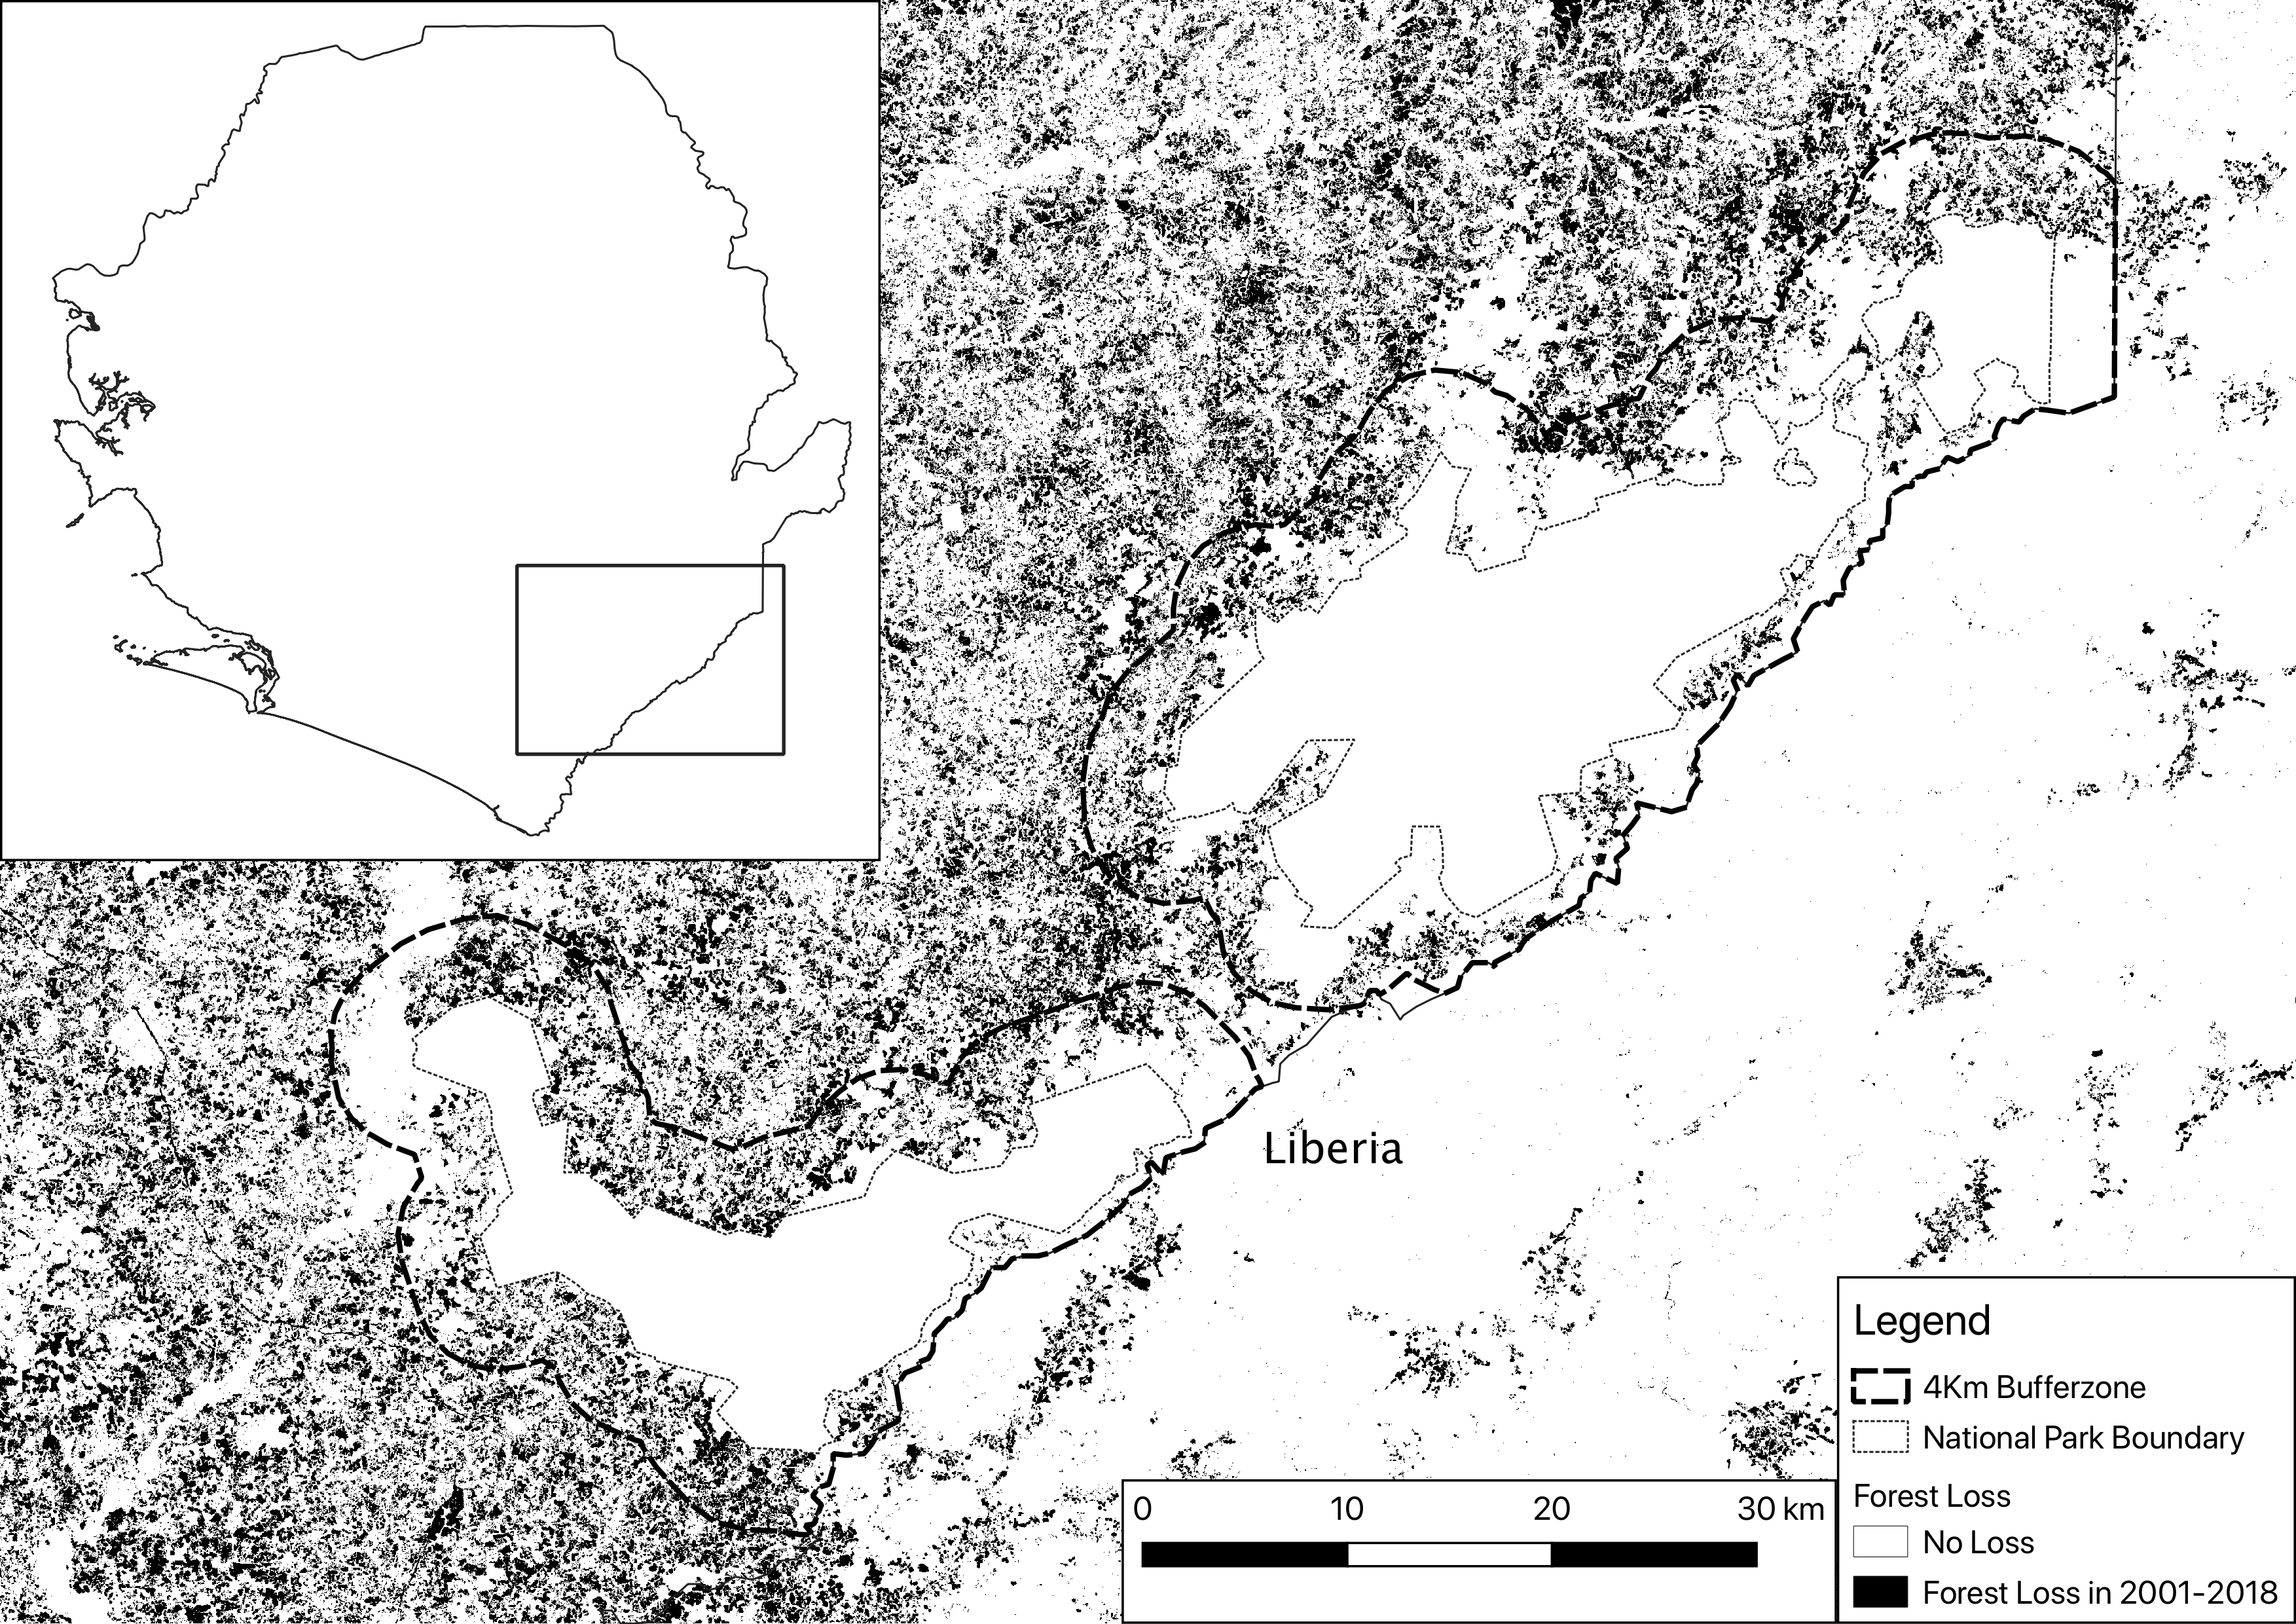
\includegraphics[width=0.7\linewidth]{3_maps/grnp_forestloss_buffer} 

}

\caption{\textbf{Yearly forest loss in the Gola Rainforest National Park area in Sierra Leone.} This figure shows for each pixel whether any deforestation took place from 2001 until 2018. The dashed line shows the 4km buffer zone in which the REDD+ programme took place. Source: Hansen 2013/UMD/Google/USGS/NASA.}\label{fig:figForestlossGola}
\end{figure}

\begin{figure}[H]

{\centering 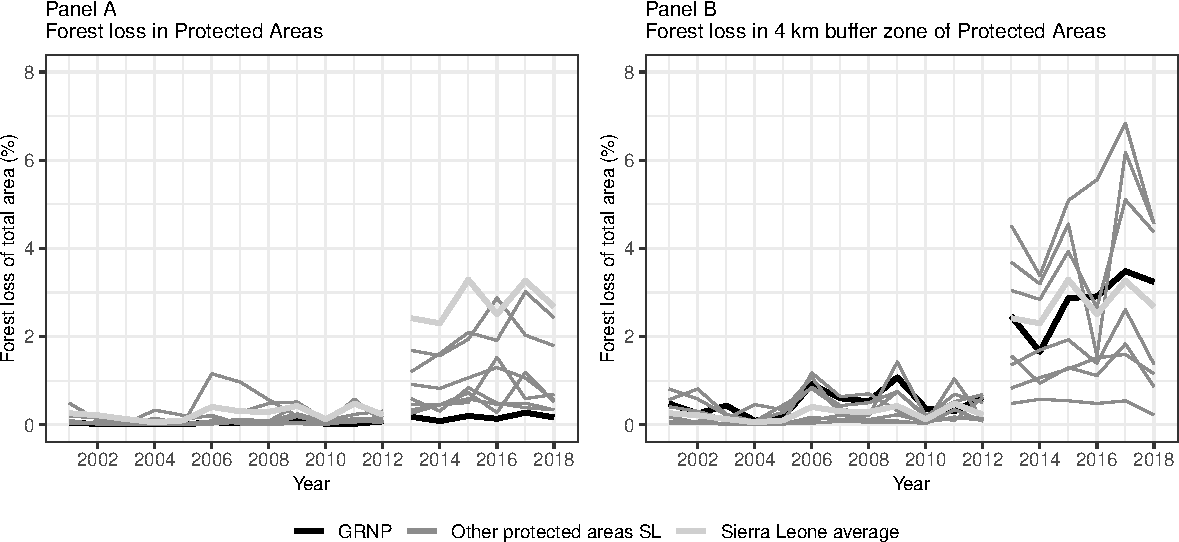
\includegraphics[width=6in]{paper_REDD_replication_files/figure-latex/figForestlossBuffer-1} 

}

\caption{\textbf{Total forest loss in Gola Rainforest National Park, other Protected Areas in Sierra Leone, and Sierra Leone as a whole.} The left panel shows total forest loss from 2001 to 2018 in 8 Protected Areas (PA) of Sierra Leone and the average for Sierra Leone. The right panel shows total forest loss from 2001 to 2018 in the 4km buffer zones of these PAs The PAs shown are Gola Rainforest National Park (GRNP), Outamba, Loma Mountains, Western Area Peninsula, Kangari Hills, Tingi Hills, Kambui Hills, and Tiwai Island. See Supplementary Table B1 for separate graphs for each PA. The break in the lines in 2013 denotes the launch of a new satellite (Landsat 8) resulting in more precise measures of forest loss. Source: Hansen 2013/UMD/Google/USGS/NASA.}\label{fig:figForestlossBuffer}
\end{figure}

\begin{figure}[H]

{\centering 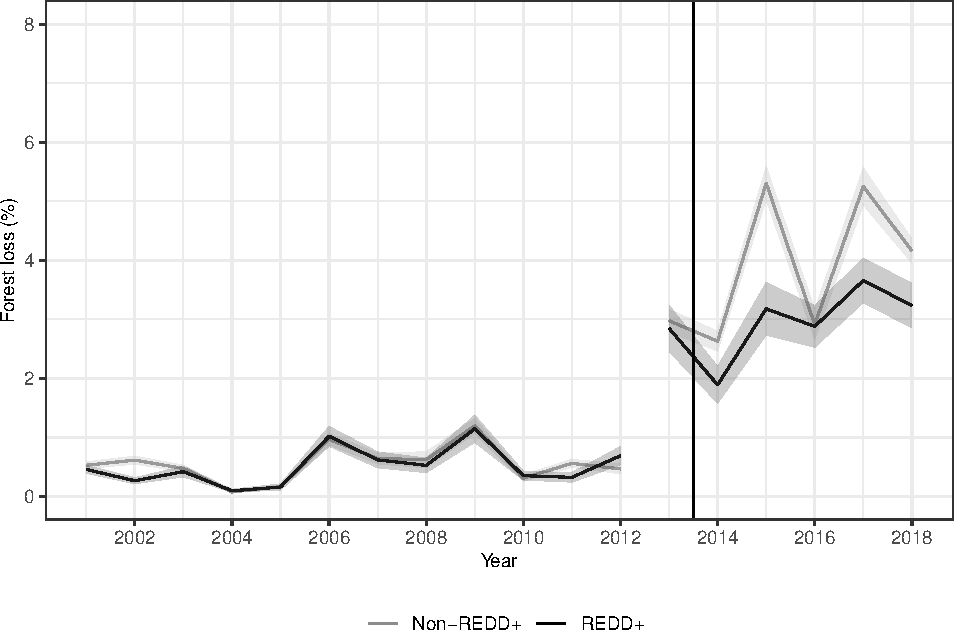
\includegraphics[width=0.9\linewidth]{paper_REDD_replication_files/figure-latex/figForestlossResults-1} 

}

\caption{\textbf{Total forest loss in REDD+ and non-REDD+ villages.} This graph shows total forest loss from 2001 to 2018 in REDD+ versus non-REDD+ villages. The village polygons are estimated using population weighted Voronoi estimations. Data are represented as mean village-level values and shaded areas denote 95 percent confidence intervals. The vertical black line indicates the start of REDD+. The break in the lines in 2013 denotes the launch of a new satellite (Landsat 8) resulting in more precise measures of forest loss. Source: Hansen 2013/UMD/Google/USGS/NASA.}\label{fig:figForestlossResults}
\end{figure}

\newpage

\hypertarget{tables}{%
\section*{Tables}\label{tables}}
\addcontentsline{toc}{section}{Tables}

\begin{table}[h]
\caption{\textbf{The impact of REDD+ on deforestation, livelihoods, and attitudes}}
\begin{center}
\begin{tabular}{l c c c}
\hline
 & Forest loss & Economic wellbeing & Attitudes \\
\hline
Post*REDD+ & $-1.032^{***}$ & $0.022$      & $-0.017$  \\
           & $(0.114)$      & $(0.132)$    & $(0.218)$ \\
Post       & $3.314^{***}$  & $0.222^{**}$ & $-0.226$  \\
           & $(0.066)$      & $(0.103)$    & $(0.138)$ \\
REDD+      & $-0.052$       & $-0.144$     & $0.176$   \\
           & $(0.033)$      & $(0.118)$    & $(0.130)$ \\
Constant   & $0.740^{***}$  & $0.000$      & $-0.000$  \\
           & $(0.017)$      & $(0.089)$    & $(0.076)$ \\
\hline
Years      & 18             & 2            & 2         \\
Villages   & $454$          & $59$         & $59$      \\
Num. obs.  & $8172$         & $1320$       & $1320$    \\
\hline
\multicolumn{4}{l}{\scriptsize{\parbox{.6\linewidth}{\vspace{2pt}$^{***}p<0.01$; $^{**}p<0.05$; $^{*}p<0.1$ based on two-sided tests.\\
       Difference-in-difference analysis using OLS regressions for forest loss (satellite data) and livelihood and conservation norms families (survey data). Post*REDD+ is the project impact coefficient. Forest loss is the percentage loss of forest (primary and secondary). The economic wellbeing family outcome is a summary index (average of z-scores) of an income index, an assets index, a durable loan size measure, and a measure for resilience. The attitudes family outcome is a summary index (average of z-scores) of a conservation attitudes index, an awareness of conservation norms index, the number of sustainable farming practices practiced, and an index for human wildlife conflict perception. Family outcomes are standardised and centred on control group at baseline and these coefficients should be interpreted as standard deviation changes. For survey outcomes (columns 2 and 3) standard errors (in parentheses) are clustered at the village-level.}}}
\end{tabular}
\label{table:coefficients}
\end{center}
\end{table}

\begin{table}[h]
\caption{\textbf{Plausible mechanisms explaining reduced deforestation from REDD+}}
\begin{center}
\begin{tabular}{l c c c c}
\hline
 & Labour acces index & Income farm wages & Income NTFP & Cocoa harvest \\
\hline
Post*REDD+ & $-0.545^{**}$ & $0.199^{*}$ & $0.343^{**}$ & $0.196$        \\
           & $(0.257)$     & $(0.106)$   & $(0.153)$    & $(0.129)$      \\
Post       & $0.365^{**}$  & $0.037$     & $0.021$      & $-0.514^{***}$ \\
           & $(0.160)$     & $(0.083)$   & $(0.106)$    & $(0.103)$      \\
REDD+      & $0.120$       & $-0.014$    & $-0.152$     & $-0.123$       \\
           & $(0.133)$     & $(0.096)$   & $(0.101)$    & $(0.126)$      \\
Constant   & $-0.000$      & $0.000$     & $0.000$      & $-0.000$       \\
           & $(0.091)$     & $(0.063)$   & $(0.087)$    & $(0.102)$      \\
\hline
Years      & 2             & 2           & 2            & 2              \\
Villages   & $59$          & $59$        & $59$         & $59$           \\
Num. obs.  & $1150$        & $1228$      & $1320$       & $1320$         \\
\hline
\multicolumn{5}{l}{\scriptsize{\parbox{.9\linewidth}{\vspace{2pt}$^{***}p<0.01$; $^{**}p<0.05$; $^{*}p<0.1$ based on two-sided tests.\\
       Difference-in-difference analysis using OLS regressions for mechanisms. Post*REDD+ is the project impact coefficient. Labour access index is an index of  three farm labour access variables (upland rice, wetland rice, and plantation) indicating to what extent there is access to labour. Income farm wages is a continuous variable (IHS transformed) measuring the yearly household income from farm wages. Income NTFP is a continuous variable (IHS transformed) measuring the yearly income from Non-Timber Forest Products collection. Cocoa harvest measures the amount of cocoa harvested in the previous year. All outcomes are standardised and centred on control group at baseline and coefficients should be interpreted as standard deviation changes. Standard errors clustered at the village level in parentheses.}}}
\end{tabular}
\label{table:coefficients}
\end{center}
\end{table}

\setcounter{table}{0} \renewcommand{\thetable}{A\arabic{table}} \setcounter{figure}{0} \renewcommand{\thefigure}{A\arabic{figure}} 
\clearpage

\setcounter{table}{0}  
\renewcommand{\thetable}{A\arabic{table}}
\setcounter{figure}{0} 
\renewcommand{\thefigure}{A\arabic{figure}}

\clearpage

\hypertarget{supplementary-information-a-literature-review}{%
\section*{Supplementary Information A: Literature
review}\label{supplementary-information-a-literature-review}}
\addcontentsline{toc}{section}{Supplementary Information A: Literature
review}

There is a growing scientific literature using BACI methods with
experimental and observational data that has assessed various Payment
for Ecosystem Service type programmes that have a carbon reduction
element (see Salzman et al.~(2018) for a review)\textsuperscript{46}.
Some of these studies use RCT methods\textsuperscript{5,32,39} while
others employ quasi-experimental techniques\textsuperscript{47--49}.
However, the programmes being evaluated are often smaller scale pilot
programmes or larger conservation PES programmes that are \emph{not}
actual certified REDD+ schemes selling credits on the voluntary market.
These studies provide lessons about the effectiveness of conservation
programmes but do not offer lessons on actual verified REDD+ projects.
All studies assessed are classified in Table A1.

Here we summarise available published work that uses BACI approaches to
assess the environmental effectiveness and livelihood impacts of REDD+
initiatives. From the studies that examine the environmental effects,
two have focused on national programmes under the UNFCCC that were never
intended to sell carbon credits\textsuperscript{50,51}. The majority of
the remaining studies discussed here explore REDD+ initiatives that were
never certified by an established verification agency (they have been
financed by grants and not through the actual sales of offsets), while
others were mostly in their early stages of development (pilots).

Bos et al., (2017) assess the deforestation performance of 23
subnational REDD+ type initiatives in Brazil, Peru, Cameroon, Tanzania,
Indonesia and Vietnam from CIFOR's Global Comparative Study on
REDD+\textsuperscript{9,12,22}. Using a BACI approach to assess
deforestation they found very modest effects of REDD+ projects. It must
be noted, however, that only 5 out of the 23 REDD+ initiatives assessed
in the CIFOR study have actually been certified to sell carbon offsets
on the voluntary carbon markets (with only 2/23 sites even ever have
sold offsets during the CIFOR study period 2010-2014). Instead they are
either jurisdictional initiatives as part of national REDD+ programmes,
or pilot projects (so called ``demonstrating activities'') or REDD+
actions funded via grants and donations (not voluntary credits). Hence,
the majority of REDD+ programmes driving the results from this CIFOR
study are substantially different in their design and level of scrutiny
as compared to the certified REDD+ projects that sell carbon offsets in
voluntary markets. Correa et al.~(2020), Cisneros et al.~(2022),
Carrilho et al.~(2022) and Simonet et al., (2019) use impact evaluation
frameworks to assess REDD+ projects in Brazil but again study
initiatives which were never certified to sell offsets in the voluntary
carbon credit markets (these are more mostly akin to PES programmes
funded by large donors)\textsuperscript{25}. Evidence derived from these
studies on the environmental effectiveness of these initiatives is
mixed. Ellis et al (2020) use BACI and synthetic control methods to
assess the impacts of subnational REDD+ initiatives in the Yucatán
Peninsula between 2010 and 2018\textsuperscript{26}. Again, none of
these schemes were financed from the sale of carbon credits on the
voluntary carbon credit markets. The authors find that the REDD+
projects have had largely insignificant impacts on deforestation rates,
though results are again more mixed and varied across location and
depending on the methods used.

In contrast, West et al (2020) assess the additionality of 12 REDD+
programmes in Brazil that were actually verified by an established
agency to sell offsets. Using synthetic control methods covering the
period between 2008 and 2017 they find that in most cases observed
deforestation rates cannot be causally attributed to REDD+ but reflect
other background factors\textsuperscript{10}. A study by Delacote et al
(2022) on similar sites in Brazil and using BACI methods concurs with
these findings\textsuperscript{28}. Similarly, Guizar‐Coutiño et
al.~(2022) using BACI with matching methods study the effectiveness of
40 certified REDD+ sites in 9 countries\textsuperscript{29}. They find
that reductions on deforestation attributable to REDD+ are generally
small with some greater impact in sites located in high-deforestation
areas. The three studies assess multiple REDD+ sites and projects, and
in doing so they inevitably standardise their impact evaluation
methodologies. This `one-size-fits-all' methodological approach (in
terms of defining the outcome variables as well as the unit of analysis)
does pose challenges in interpreting and comparing the results between
sites. Also, neither of these papers have access to suitable
socioeconomic data to explore livelihood impacts and cannot study the
mechanisms behind the results over effectiveness.

Rigorous BACI style evaluation studies of livelihood impacts remain
scant. A rare exemption comes from Duchelle et al (2017) and Simonet et
al (2017) that use multi-country data from the data CIFOR's Global
Comparative Study, which as noted above studies mostly different type of
REDD+ initiatives that are not certified to sell carbon
credits\textsuperscript{21,23}. Results show that REDD+ interventions
had a minimal impact on household and village level well-being and
income indicators. Similarly, a study by Jagger and Rana (2017) uses
publicly available secondary data to assess livelihood impacts of 18
REDD+ projects in Indonesia\textsuperscript{30}. They find evidence of
negative impacts on livelihood measures though most of the programmes
evaluated were in a rather early stage of development (pilots) or did
not have certification for selling offsets. In a recent review of the
literature by Duchelle et al (2018), the authors also paint a rather
less favourable picture of the impacts of REDD + on livelihoods, though
the literature they refer to relies on less rigorous statistical methods
that do not follow a BACI approach\textsuperscript{13}. Also, most of
the REDD+ projects that are discussed in this review have not been
certified to sell carbon credits (and hence have lower standards to
begin with when it comes to meeting social objectives).

\clearpage
\begin{landscape}
\begin{table}[!h]

\caption{\label{tab:tablelit}\textbf{Summary of REDD+ impact evaluation literature}}
\centering
\fontsize{5}{7}\selectfont
\begin{threeparttable}
\begin{tabular}[t]{>{\raggedright\arraybackslash}p{4em}|>{\raggedright\arraybackslash}p{4em}|>{\raggedright\arraybackslash}p{5em}|>{\raggedright\arraybackslash}p{4em}|>{\raggedright\arraybackslash}p{4em}|>{\raggedright\arraybackslash}p{4em}|>{\raggedright\arraybackslash}p{6em}|>{\raggedright\arraybackslash}p{6em}|>{\raggedright\arraybackslash}p{6em}|>{\raggedright\arraybackslash}p{5em}|>{\raggedright\arraybackslash}p{5em}|>{\raggedright\arraybackslash}p{5em}|>{\raggedright\arraybackslash}p{5em}|>{\raggedright\arraybackslash}p{4em}}
\hline
\textbf{Reference} & \textbf{Method} & \textbf{Country (sites)} & \textbf{Time period} & \textbf{Program} & \textbf{Voluntary carbon credits sold} & \textbf{Cash vs non-cash incentives} & \textbf{Deforestation indicator} & \textbf{Deforestation impact*} & \textbf{\% avoided deforestation} & \textbf{Socio- economic indicator} & \textbf{Socio- economic impact*} & \textbf{Mechanism} & \textbf{Cost}\\
\hline
Bos et al. (2017) & BACI (DID) & Brazil, Peru, Cameroon, Tanzania, Indonesia, Vietnam (23 sites)** & 2-9 years & REDD+ initiatives & Mostly no & Mix of incentives (e.g. livelihoods intervention) and disincentives (e.g. fines, access restrictions) & Satellite data: tree cover loss & + (tree cover loss) & Not assessed & Not assessed & Not assessed & Not assessed & Not assessed\\
Carrilho et al. (2022) & BACI (DID) & Brazil (1 site) & 2 years & REDD+ initiative with a PES-component & No & Mix of conditional incentives (e.g. cash, awareness raising, sustainable livelihood alternatives) & Satellite data: tree cover loss & + (tree cover loss) & 7.80\% - 10.32\% & Subjective well-being & + & Profitability in pasture and agricultural plots & Not assessed\\
Cisneros et al. (2022) & BACI (matching) & Brazil (1 site) & 2008-2015 & PES & No & Conditional cash & Satellite data: tree cover loss & + (tree cover loss) & 0.1 & Not assessed & Not assessed & Not assessed & Not assessed\\
Correa et al. (2020) & BACI (Syn. Control) & Brazil (1 site) & 2011-2018 & Amazon Fund initiative & No & Mix of positive incentives on the municipality and farm level & Satellite data: tree cover loss & No impact & No impact & Not assessed & Not assessed & Land registration, restoration, output diversification in agriculture, intensification of cattle production & Not assessed\\
Delacote et al. (2022) & BACI (DID-matching) & Brazil (6 sites) & Different time frames & REDD+ initiatives & Yes & Mix of incentives & Satellite data: tree cover loss & No impact at 5 sites, 1 site + & Small impact for 1 site & Not assessed & Not assessed & Not assessed & Not assessed\\
Duchelle et al. (2017) & BACI (DID) & Brazil, Peru, Cameroon, Tanzania, Indonesia, Vietnam (17 sites)** & 2 years & REDD+ initiatives & Mostly no & Mix of incentives (e.g. livelihoods intervention) and disincentives (e.g. fines, access restrictions) & Self-reported: forest clearing; tenure security & +/- (forest clearing) +/- (tenure security) & Not assessed & Subjective well-being & +/- & Not assessed & Not assessed\\
Ellis et al. (2020) & BACI (DID, Syn. Control) & Mexico (various sites in Yucatan) & Vary in length & REDD+ initiatives & No & Mix of incentives & Satellite data: tree cover loss & DID: no impact; Syn. Control: +/- & - & Not assessed & Not assessed & Not assessed & Not assessed\\
\hline
\end{tabular}
\begin{tablenotes}
\item \textit{Note: } 
\item *+ positive impact (i.e. reduced deforestation; increase in social welfare); - negative impact (i.e. increased deforestation; decrease in social welfare); +/- mixed impact (i.e. increase/decrease of relevant indicator); no impact. ‘Not assessed’ means that the relevant information was not collected or not evaluated. **Data from CIFOR’s Global Comparative Study on REDD+. Only 5/23 of the Redd initiatives studied were ever certified to sell credits in the voluntary market. Information on the methods and results collected from the original publication. Information concerning the REDD+ intervention and whether they were certified to sell offsets on the voluntary carbon market was cross from the REDD initiative websites, the International Database on REDD+ Projects (https://www.reddprojectsdatabase.org/), and from CIFOR’s global database resources for REDD+ (https://www.cifor-icraf.org/gcs/redd-map/).
\end{tablenotes}
\end{threeparttable}
\end{table}

\clearpage
\begin{table}[!h]
\centering\begingroup\fontsize{5}{7}\selectfont

\begin{threeparttable}
\begin{tabular}{>{\raggedright\arraybackslash}p{4em}|>{\raggedright\arraybackslash}p{4em}|>{\raggedright\arraybackslash}p{5em}|>{\raggedright\arraybackslash}p{4em}|>{\raggedright\arraybackslash}p{4em}|>{\raggedright\arraybackslash}p{4em}|>{\raggedright\arraybackslash}p{6em}|>{\raggedright\arraybackslash}p{6em}|>{\raggedright\arraybackslash}p{6em}|>{\raggedright\arraybackslash}p{5em}|>{\raggedright\arraybackslash}p{5em}|>{\raggedright\arraybackslash}p{5em}|>{\raggedright\arraybackslash}p{5em}|>{\raggedright\arraybackslash}p{4em}}
\hline
\textbf{Reference} & \textbf{Method} & \textbf{Country (sites)} & \textbf{Time period} & \textbf{Program} & \textbf{Voluntary carbon credits sold} & \textbf{Cash vs non-cash incentives} & \textbf{Deforestation indicator} & \textbf{Deforestation impact*} & \textbf{\% avoided deforestation} & \textbf{Socio- economic indicator} & \textbf{Socio- economic impact*} & \textbf{Mechanism} & \textbf{Cost}\\
\hline
Groom et al. (2022) & BACI (DDD, matching) & Indonesia (nationwide) & 2011-2018 & National REDD+ & No & Mix of incentives & Satellite data: tree cover loss & + tree cover loss, dryland forest; no impact on peatland forest & 0.65\% (dryland forest) & Not assessed & Not assessed & Not assessed & Cost: below \$5 per averted tCO2\\
Guizar-Coutino et al. (2022) & BACI (matching) & Global (40 sites) & 5 years & REDD+ initiatives & Yes & Mix of incentives & Satellite data: tree cover loss & + (tree cover loss) & Mean across sites: 0.14\% & Not assessed & Not assessed & Not assessed & Not assessed\\
Jagger and Rana (2017) & BACI (DID, matching) & Indonesia (18 sites) & Different time frames & REDD+ initiatives & Mostly No & Mix of incentives & Satellite data: tree cover loss & No impact & No impact & Customary land burning, incidence of poverty, access to free health services, fuel usage, mobile phone service, presence of internet & Mixed results & Not assessed & Not assessed\\
Roopsind et al. (2019) & BACI (Syn. control) & Guyana (nationwide) & 5 years & National REDD+ & No & Conditional cash/non-cash & Satellite data: tree cover loss & + (tree cover loss) & 0.00031 & Not assessed & Not assessed & Not assessed & \$19.53 per averted tCO2\\
Sunderlin et al. (2017) & BACI (DID) & Brazil, Peru, Cameroon, Tanzania, Indonesia, Vietnam (22 sites)** & 2 years & REDD+ initiatives & Mostly no & Mix of incentives (e.g. livelihoods intervention) and disincentives (e.g. fines, access restrictions) & Not assessed & Not assessed & Not assessed- & Subjective well-being. Income sufficiency & No impact & Not assessed & Not assessed\\
Simonet et al. (2019) & BACI (DID) & Brazil (1 site)** & 1 year & REDD+ pilot with a PES-component & No & Conditional cash & Satellite data: tree cover loss & + (tree cover loss) & 0.054 & Not assessed & Not assessed & Additional wage labor income. Intensification of livestock. Proportion of cropland/pasture & \$0.84 per averted tCO2\\
West et al. (2020) & BACI (Syn. control) & Brazil (12 sites) & Vary in length from 2008-2017 & REDD+ initiatives & Yes & Not indicated & Satellite data: tree cover loss & No impact & No impact & Not assessed & Not assessed & Not assessed & Not assessed\\
\hline
\end{tabular}
\begin{tablenotes}
\item \textit{Note: } 
\item *+ positive impact (i.e. reduced deforestation; increase in social welfare); - negative impact (i.e. increased deforestation; decrease in social welfare); +/- mixed impact (i.e. increase/decrease of relevant indicator); no impact. ‘Not assessed’ means that the relevant information was not collected or not evaluated. **Data from CIFOR’s Global Comparative Study on REDD+. Only 5/23 of the Redd initiatives studied were ever certified to sell credits in the voluntary market. Information on the methods and results collected from the original publication. Information concerning the REDD+ intervention and whether they were certified to sell offsets on the voluntary carbon market was cross from the REDD initiative websites, the International Database on REDD+ Projects (https://www.reddprojectsdatabase.org/), and from CIFOR’s global database resources for REDD+ (https://www.cifor-icraf.org/gcs/redd-map/).
\end{tablenotes}
\end{threeparttable}
\endgroup{}
\end{table}

\end{landscape}
\clearpage

\setcounter{table}{0}  
\renewcommand{\thetable}{B\arabic{table}}
\setcounter{figure}{0} 
\renewcommand{\thefigure}{B\arabic{figure}}

\hypertarget{supplementary-information-b-forest-loss-in-protected-areas}{%
\section*{Supplementary Information B: Forest loss in Protected
Areas}\label{supplementary-information-b-forest-loss-in-protected-areas}}
\addcontentsline{toc}{section}{Supplementary Information B: Forest loss
in Protected Areas}

\begin{figure}[H]

{\centering 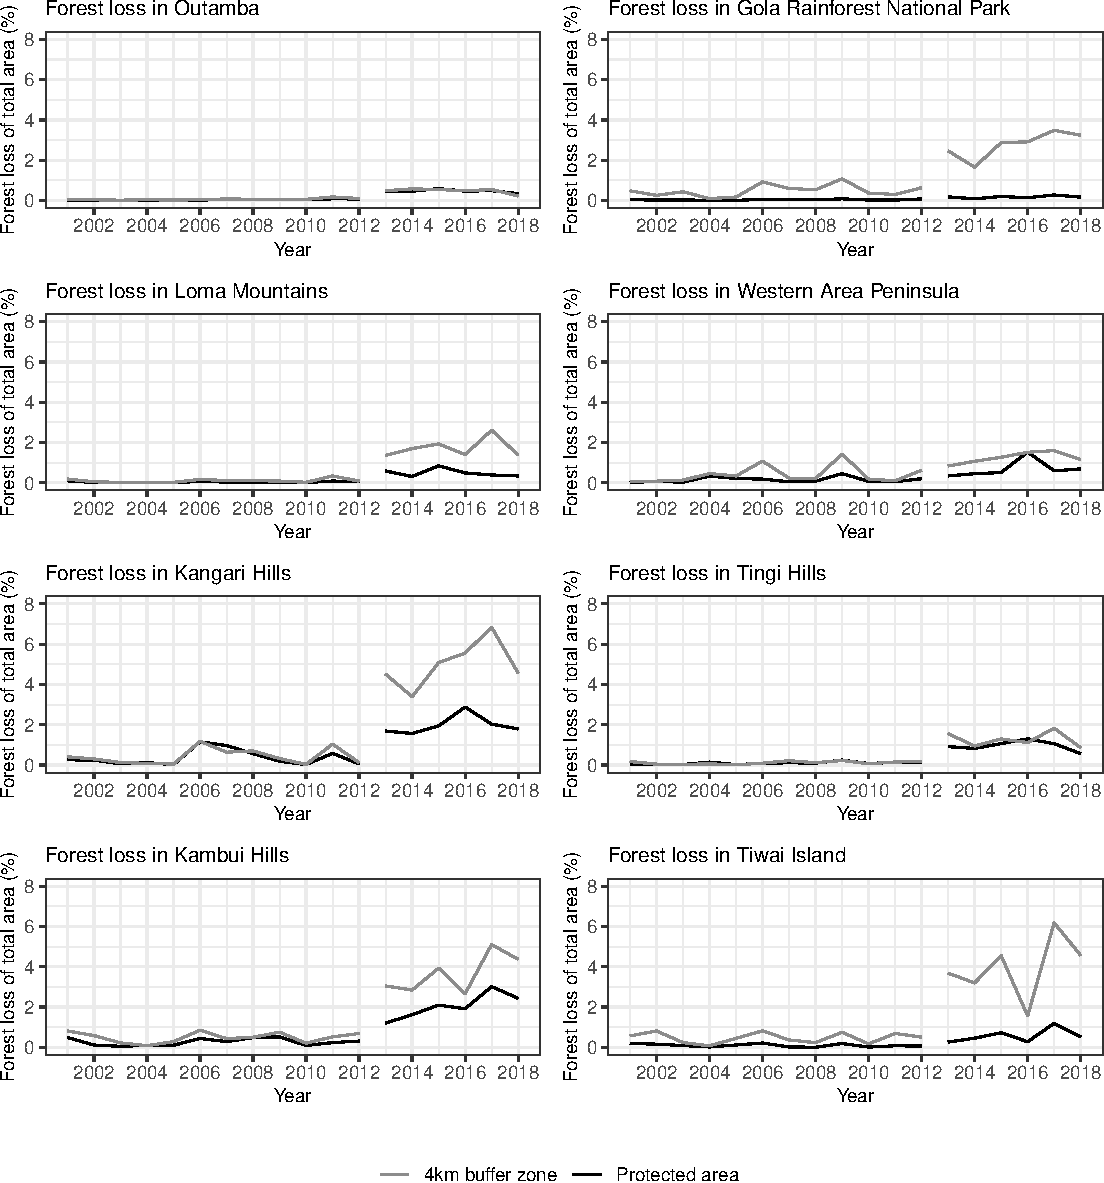
\includegraphics{paper_REDD_replication_files/figure-latex/figForestlossPa-1} 

}

\caption{\textbf{Yearly forest loss in the Protected Areas in Sierra Leone.} This graph shows total forest loss from 2001 to 2018 in Protected Areas of Sierra Leone and their 4 km buffer zones. The break in the lines in 2013 denotes the launch of a new satellite (Landsat 8) resulting in more precise measures of forest loss. Protected area definitions come from the Sierra Leonean government. Source: Hansen 2013/UMD/Google/USGS/NASA.}\label{fig:figForestlossPa}
\end{figure}

\begin{figure}[H]

{\centering 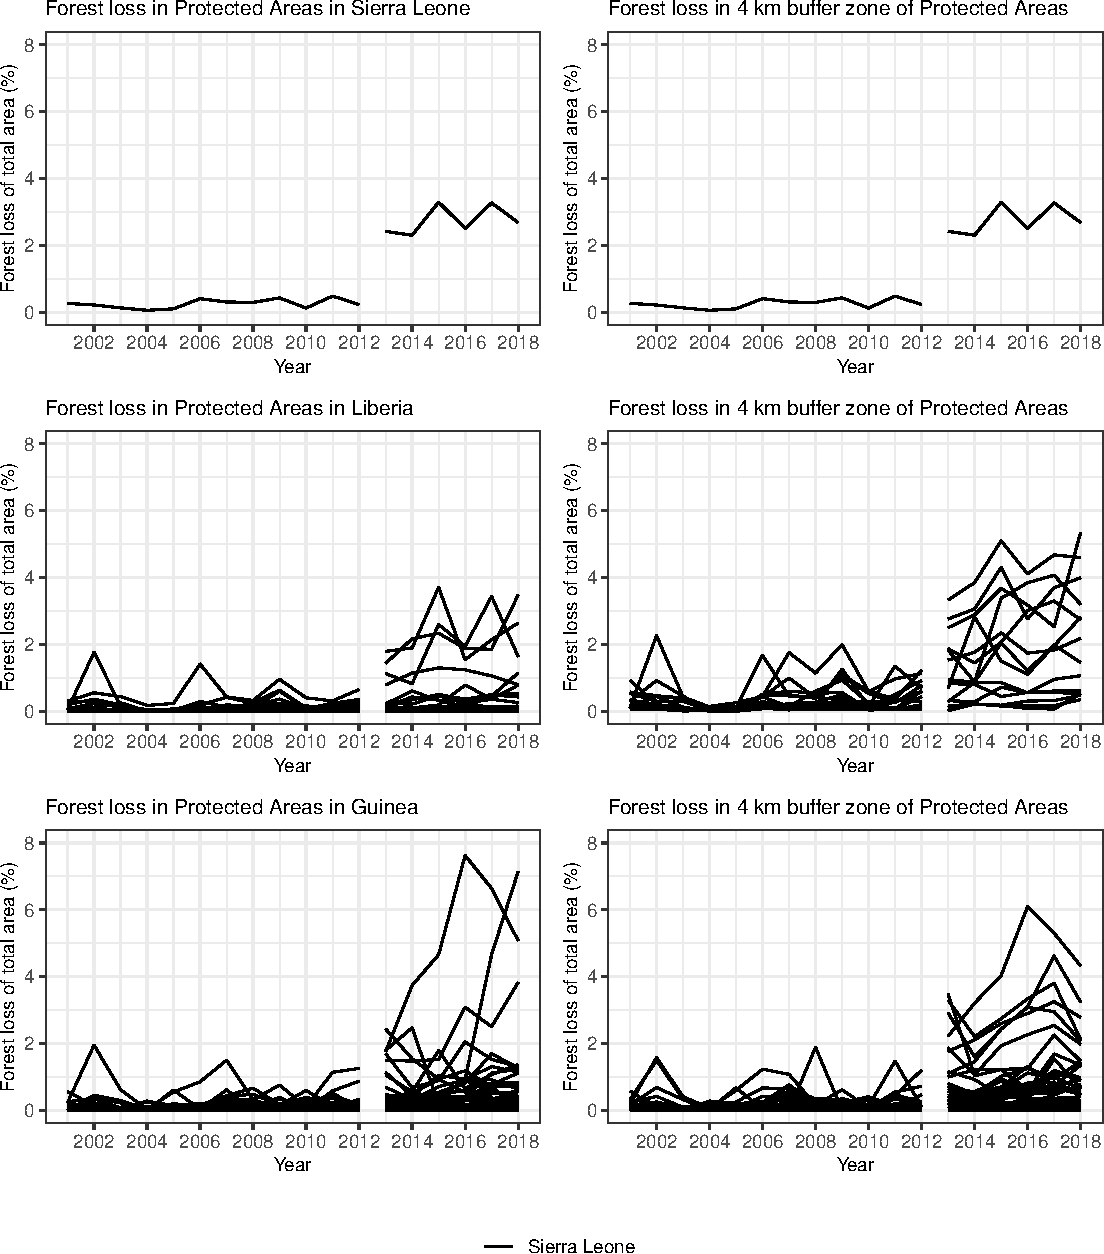
\includegraphics{paper_REDD_replication_files/figure-latex/figForestlossCountry-1} 

}

\caption{\textbf{Yearly forest loss in the Protected Areas in Sierra Leone, Liberia, and Guinea.} This graph shows forest loss from 2001 to 2018 in Protected Areas of Sierra Leone, Liberia, and Guinea and their 4 km buffer zones. The break in the lines in 2013 denotes the launch of a new satellite (Landsat 8) resulting in more precise measures of forest loss. Protected area definitions come from the Worldwide Database on Protected Areas. We exclude all polygons below a certain size (10.000 pixels) for readability of the graph and because we are unsure of the reliability of these data. Source of data: Hansen 2013/UMD/Google/USGS/NASA/WDPA.}\label{fig:figForestlossCountry}
\end{figure}
\newpage
\setcounter{table}{0}  
\renewcommand{\thetable}{C\arabic{table}}
\setcounter{figure}{0} 
\renewcommand{\thefigure}{C\arabic{figure}}

\hypertarget{supplementary-information-c-redd-intervention-in-sierra-leone}{%
\section*{Supplementary Information C: REDD+ intervention in Sierra
Leone}\label{supplementary-information-c-redd-intervention-in-sierra-leone}}
\addcontentsline{toc}{section}{Supplementary Information C: REDD+
intervention in Sierra Leone}

GRC (or its predecessor the Gola Rainforest Program) have been managing
the GRNP for over 20 years. Activities intensified under a 2007-2012
funding cycle that included a set of livelihood and conservation
activities. As part of the Community Development Fund so-called Forest
Edge Communities (villages that lie within 1.6km of the park boundaries)
received a once off small-scale livelihoods program in 2011 (see Voors
et al.~2018)\textsuperscript{52}. Below, as a robustness exercise, we
drop these villages from the analysis, see Table F4. Another livelihood
program, implemented as a randomised trial ran 2011-2013 and focused on
a second `ring' of villages that lie in the 1--7-mile band from the park
boundary (see in Wilebore et al.~2019). Here the authors find livelihood
activities increased deforestation in treatment areas, compared to
control areas (that lie within the same distance from the forest). Since
these activities were randomly implemented, and thus favoured villages
at varying distances from the National Park there is no reason to assume
they systematically favoured villages in the current REDD+ area.

The current REDD+ activities are directed specifically to communities
located in the 4 km buffer zone and focus on reducing extensive
agriculture (i.e.~upland rice farming) and moving towards more
forest-friendly crops (e.g.~cocoa and wetland rice), thereby aiming to
reduce pressure on the buffer zone, which in turn reduces pressure on
the GRNP. The three main REDD+ activities exclusively in the buffer zone
are:

\emph{Agricultural programmes}: Agricultural programmes consists mainly
of training on crop production. Generally, a demonstration plot is
established and farmers are invited to observe and learn new methods to
improve yields. This is done specifically for wetland rice, groundnuts
and several vegetables. Crucially, the programmes do not include upland
rice, the most commonly produced crop, as it requires slash-and-burn
agriculture and large amounts of land. In fact, GRC actively discourages
upland rice farming.

\emph{Cocoa programmes}: Within the cocoa programmes, GRC provides
training on production, farm management, and post-harvest processing.
Cocoa in Sierra Leone is considered a `forest-friendly' crop: cocoa
farms are often created in secondary forests with very minimal land
clearing. The shade provided by trees (which are rarely cut down)
reduces the need for extensive weeding. GRC's activities are run through
farmer field schools and by training master farmers within the
communities. In addition, GRC established farmer associations of which
community members of REDD+ communities can become a member if they own a
cocoa plantation. These farmer associations are equipped with buying
stations and trained buying officers. These buying officers are
responsible for sourcing the cocoa from the REDD+ communities at a
somewhat higher price. This price is based on the market price in the
regional cocoa hub minus a transportation fee (This price is typically
higher than the local price). The cocoa is used to produce high-quality
single origin niche chocolate which is sold at a premium. Some of this
premium is returned to the cocoa farmers. Farmers are still free to sell
cocoa to any other trader.

\emph{Savings and Lending Associations}: GRC also established Village
Savings and Lending Associations (VSLA) as part of the REDD+ programme.
The aim is to improve financial access and facilitate investment,
thereby increasing resilience. Participation is voluntarily and
participants can either save money or take out a loan from the saved
money. The size of the loan depends on how much was contributed. The
VSLA is run by a trained committee that decides on the interest rates
for saving and lending and on membership. In addition, the VSLA has a
separate fund for emergency loans. Members also receive business
training and financial literacy training through the VSLA. GRC's role
has been to establish the VSLAs and provide training on their
functioning. They are currently only involved in monitoring and
providing support when necessary.

In Table C1 below, the proportion of villages that received each
intervention is shown. Some villages received multiple interventions.
Because these interventions were not randomly assigned to communities,
we estimate the impact of the entire REDD+ programme.

\begin{table}[!h]

\caption{\label{tab:tabIntervention}\textbf{Interventions in sample of REDD+ villages}}
\centering
\begin{threeparttable}
\begin{tabular}[t]{l>{\raggedright\arraybackslash}p{8em}>{\raggedright\arraybackslash}p{4em}}
\toprule
\textbf{Intervention} & \textbf{\# REDD+ vil. with intervention} & \textbf{\% of total sample}\\
\midrule
Agricultural intervention & 20 & 69\%\\
Cocoa intervention & 24 & 83\%\\
Village savings and loans associations & 18 & 62\%\\
REDD+ villages in sample & 29 & \\
\bottomrule
\end{tabular}
\begin{tablenotes}
\item \textit{Note: } 
\item Implementation of REDD+ interventions from 2014-2018. We only have data on which interventions were implemented in a randomly selected sample of 29 REDD+ villages for which we have survey data
\end{tablenotes}
\end{threeparttable}
\end{table}

\newpage
\setcounter{table}{0}  
\renewcommand{\thetable}{D\arabic{table}}
\setcounter{figure}{0} 
\renewcommand{\thefigure}{D\arabic{figure}}
\clearpage

\hypertarget{supplementary-information-d-data-generation-and-descriptive-statistics}{%
\section*{Supplementary Information D: Data generation and descriptive
statistics}\label{supplementary-information-d-data-generation-and-descriptive-statistics}}
\addcontentsline{toc}{section}{Supplementary Information D: Data
generation and descriptive statistics}

The data used for this paper stems from satellite imagery and several
waves of household survey data. The data collection and analysis
strategy was based on a REDD+ project monitoring plan written in 2013,
before the start of the project. A formal pre-analysis plan (OSF id:
8n7h6 available at osf.io/8n7h6) was registered before the endline data
was cleaned and analysed, but after data was collected. All satellite
and household survey outcomes as defined in the pre-analysis plan can be
found Table D1. The section below details the data generation process,
descriptive statistics for the household survey data, and other
covariates and explores the parallel trends assumption.

\begin{table}[!h]

\caption{\label{tab:outcomes}\textbf{Family indicators and outcomes}}
\centering
\begin{threeparttable}
\begin{tabular}[t]{l>{\raggedright\arraybackslash}p{30em}}
\toprule
Outcome & Description\\
\midrule
\addlinespace[0.3em]
\multicolumn{2}{l}{\textbf{Primary outcomes}}\\
\textbf{\hspace{1em}Forest loss} & \textbf{Loss of forest (vegetation cover of >5m over >30\% of the site) at a satellite resolution of 30m}\\
\hspace{1em}Primary forest loss & Loss of old growth forest (classified through extensive ground measurements)\\
\hspace{1em}Secondary forest loss & Loss of secondary forest measured as conversiom of fallow to production agriculture\\
\textbf{\hspace{1em}Economic wellbeing family} & \textbf{Summary index - average of z-scores of all components}\\
\hspace{1em}Income index & Summary index - average of z-scores of total income and expenditures in previous calendar year\\
\hspace{1em}Assets index & Assets summary index - weighted average of z-scores of all assets owned in previous calendar year\\
\hspace{1em}Durable loan size & Amount borrowed for durable investments in previous calendar year (1000 Le)\\
\hspace{1em}Resilience & Able to get money to deal with emergency in previous calendar year (y/n)\\
\textbf{\hspace{1em}Conservation norms family} & \textbf{Summary index - average of z-scores of all components}\\
\hspace{1em}Conservation attitudes & Agreement with pro-conservation statements (sum of Likert questions, 4-20)\\
\hspace{1em}Awareness of conservation norms & Number of questions about rules correctly answered (0-5)\\
\hspace{1em}Sustainable farming practices & Number of sustainable farming practices used (0-4)\\
\hspace{1em}Human wildlife conflict perceptions & Perception of how big of a problem crop raiding is  (Scale, 0-3)\\
\addlinespace[0.3em]
\multicolumn{2}{l}{\textbf{Mechanisms}}\\
\hspace{1em}Labour acces index & Average of three farm labour access variables (upland rice, wetland rice, plantation) (scale, 0-3)\\
\hspace{1em}Income farm wages & Income from farm wages in previous calendar year (1000 Le)\\
\hspace{1em}Income NTFP & Income from non-timber forest products in previous calendar year (1000 Le)\\
\hspace{1em}Cocoa harvest & Total cocoa production in previous calendar year (kg)\\
\bottomrule
\end{tabular}
\begin{tablenotes}
\item \textit{Note: } 
\item Summary indices are created following Kling et al. 2007. All variables are rescaled in the analysis so a higher value=better.
\end{tablenotes}
\end{threeparttable}
\end{table}

\hypertarget{satellite-data}{%
\subsection*{Satellite data}\label{satellite-data}}
\addcontentsline{toc}{subsection}{Satellite data}

We use Hansen et al.~(2013) global deforestation dataset with yearly
data on forest loss. We use data from the 2001-2018 period. The Hansen
dataset maps global tree cover extent, loss and gain at a spatial
resolution of 30m\textsuperscript{42}, based on Landsat satellite
images. Trees are defined as all vegetation taller than 5m in height and
forest as an area with \textgreater50\% trees. Forest loss is defined as
a stand-replacement disturbance (i.e.~the complete removal of tree
canopy).

There is one discontinuity in the Hansen dataset worth mentioning.
Following the launch of the Landsat 8 satellite in 2013, more precise
satellite imagery became available. In the data for Sierra Leone we
especially see higher forest loss detected from 2013 onwards, coinciding
with the addition of Landsat 8 data. To rule out that this discontinuity
drives the result our forest loss result, we run multiple robustness
analysis in Supplementary Information F.

We use the Hansen dataset to aggregate yearly forest loss estimates at
the village level. As administrative boundaries in Sierra Leone are not
available at the village-level, we use the the estimated village
boundaries by Wilebore and Coomes (2016)\textsuperscript{43} to assign
forest loss to villages. Wilebore and Coomes obtain point-locations of
all 454 villages in the seven chiefdoms in which the GRNP lies using
existing maps or remotely sensed imagery. Of these, 228 villages are
surveyed collecting census data and villages are asked to estimate of
the village area. For 98 of these villages, handheld GPS devices are
used to record point coordinates of the village boundaries. This data is
used to verify the predicted village boundaries.

The authors subsequently use three models (circular neighbourhood
buffers, unweighted Voronoi polygons, and weighted Voronoi polygons) to
predict village boundaries, using the estimated village sizes collected
in the survey. Performance of the three models is assessed by comparing
the predicted boundaries to the 98 known village boundary point
coordinates. Weighted Voronoi polygons perform much better than the
other two models (the correlation of predicted and actual boundaries is
0.68, as compared to 0.18 for unweighted Voronoi polygons). In this
model, the authors first draw simple Voronoi polygons for all villages.
This process assigns every pixel in the landscape to the closest village
point location, thereby dividing the landscape into regions. The 228
surveyed villages are then assigned a weight based on whether they are
smaller (\textless1) or larger (\textgreater1) than the estimated area
in the village survey. Unsurveyed villages receive a weight of 1. These
weights are then used to adjust the predicted village size.

In our analysis we use the weighted Voronoi polygons as estimated by
Wilebore and Coomes as shown in Figure D1. We also run a robustness
check excluding all villages that were not surveyed (and thus received a
weight of 1) in Table F5.

Following our pre-analysis plan we classify forests loss as changes in
primary and secondary forests. Primary forest loss is loss of old growth
forest and secondary forest loss measures conversion of fallow to
production agriculture. Both were classified through extensive ground
measurements, which were done in 2013\textsuperscript{43} and data is
thus available from 2013-2018.

In Figure D2 we run an event-study model in which we estimate
year-specific effects of REDD+ using a fixed-effects OLS estimation. We
see that in the years prior to the implementation of REDD+ (the dashed
line) the difference between levels in deforestation between REDD+ and
non-REDD+ villages are generally not significant. For one year (2002)
the difference is small (0.3\%) and significant. However, we do not
think this represents a major deviation from the observed parallel
trends. In the years after the implementation of REDD+ the differences
are instead large, negative and highly significant (for all years except
2016).

\begin{figure}[H]

{\centering 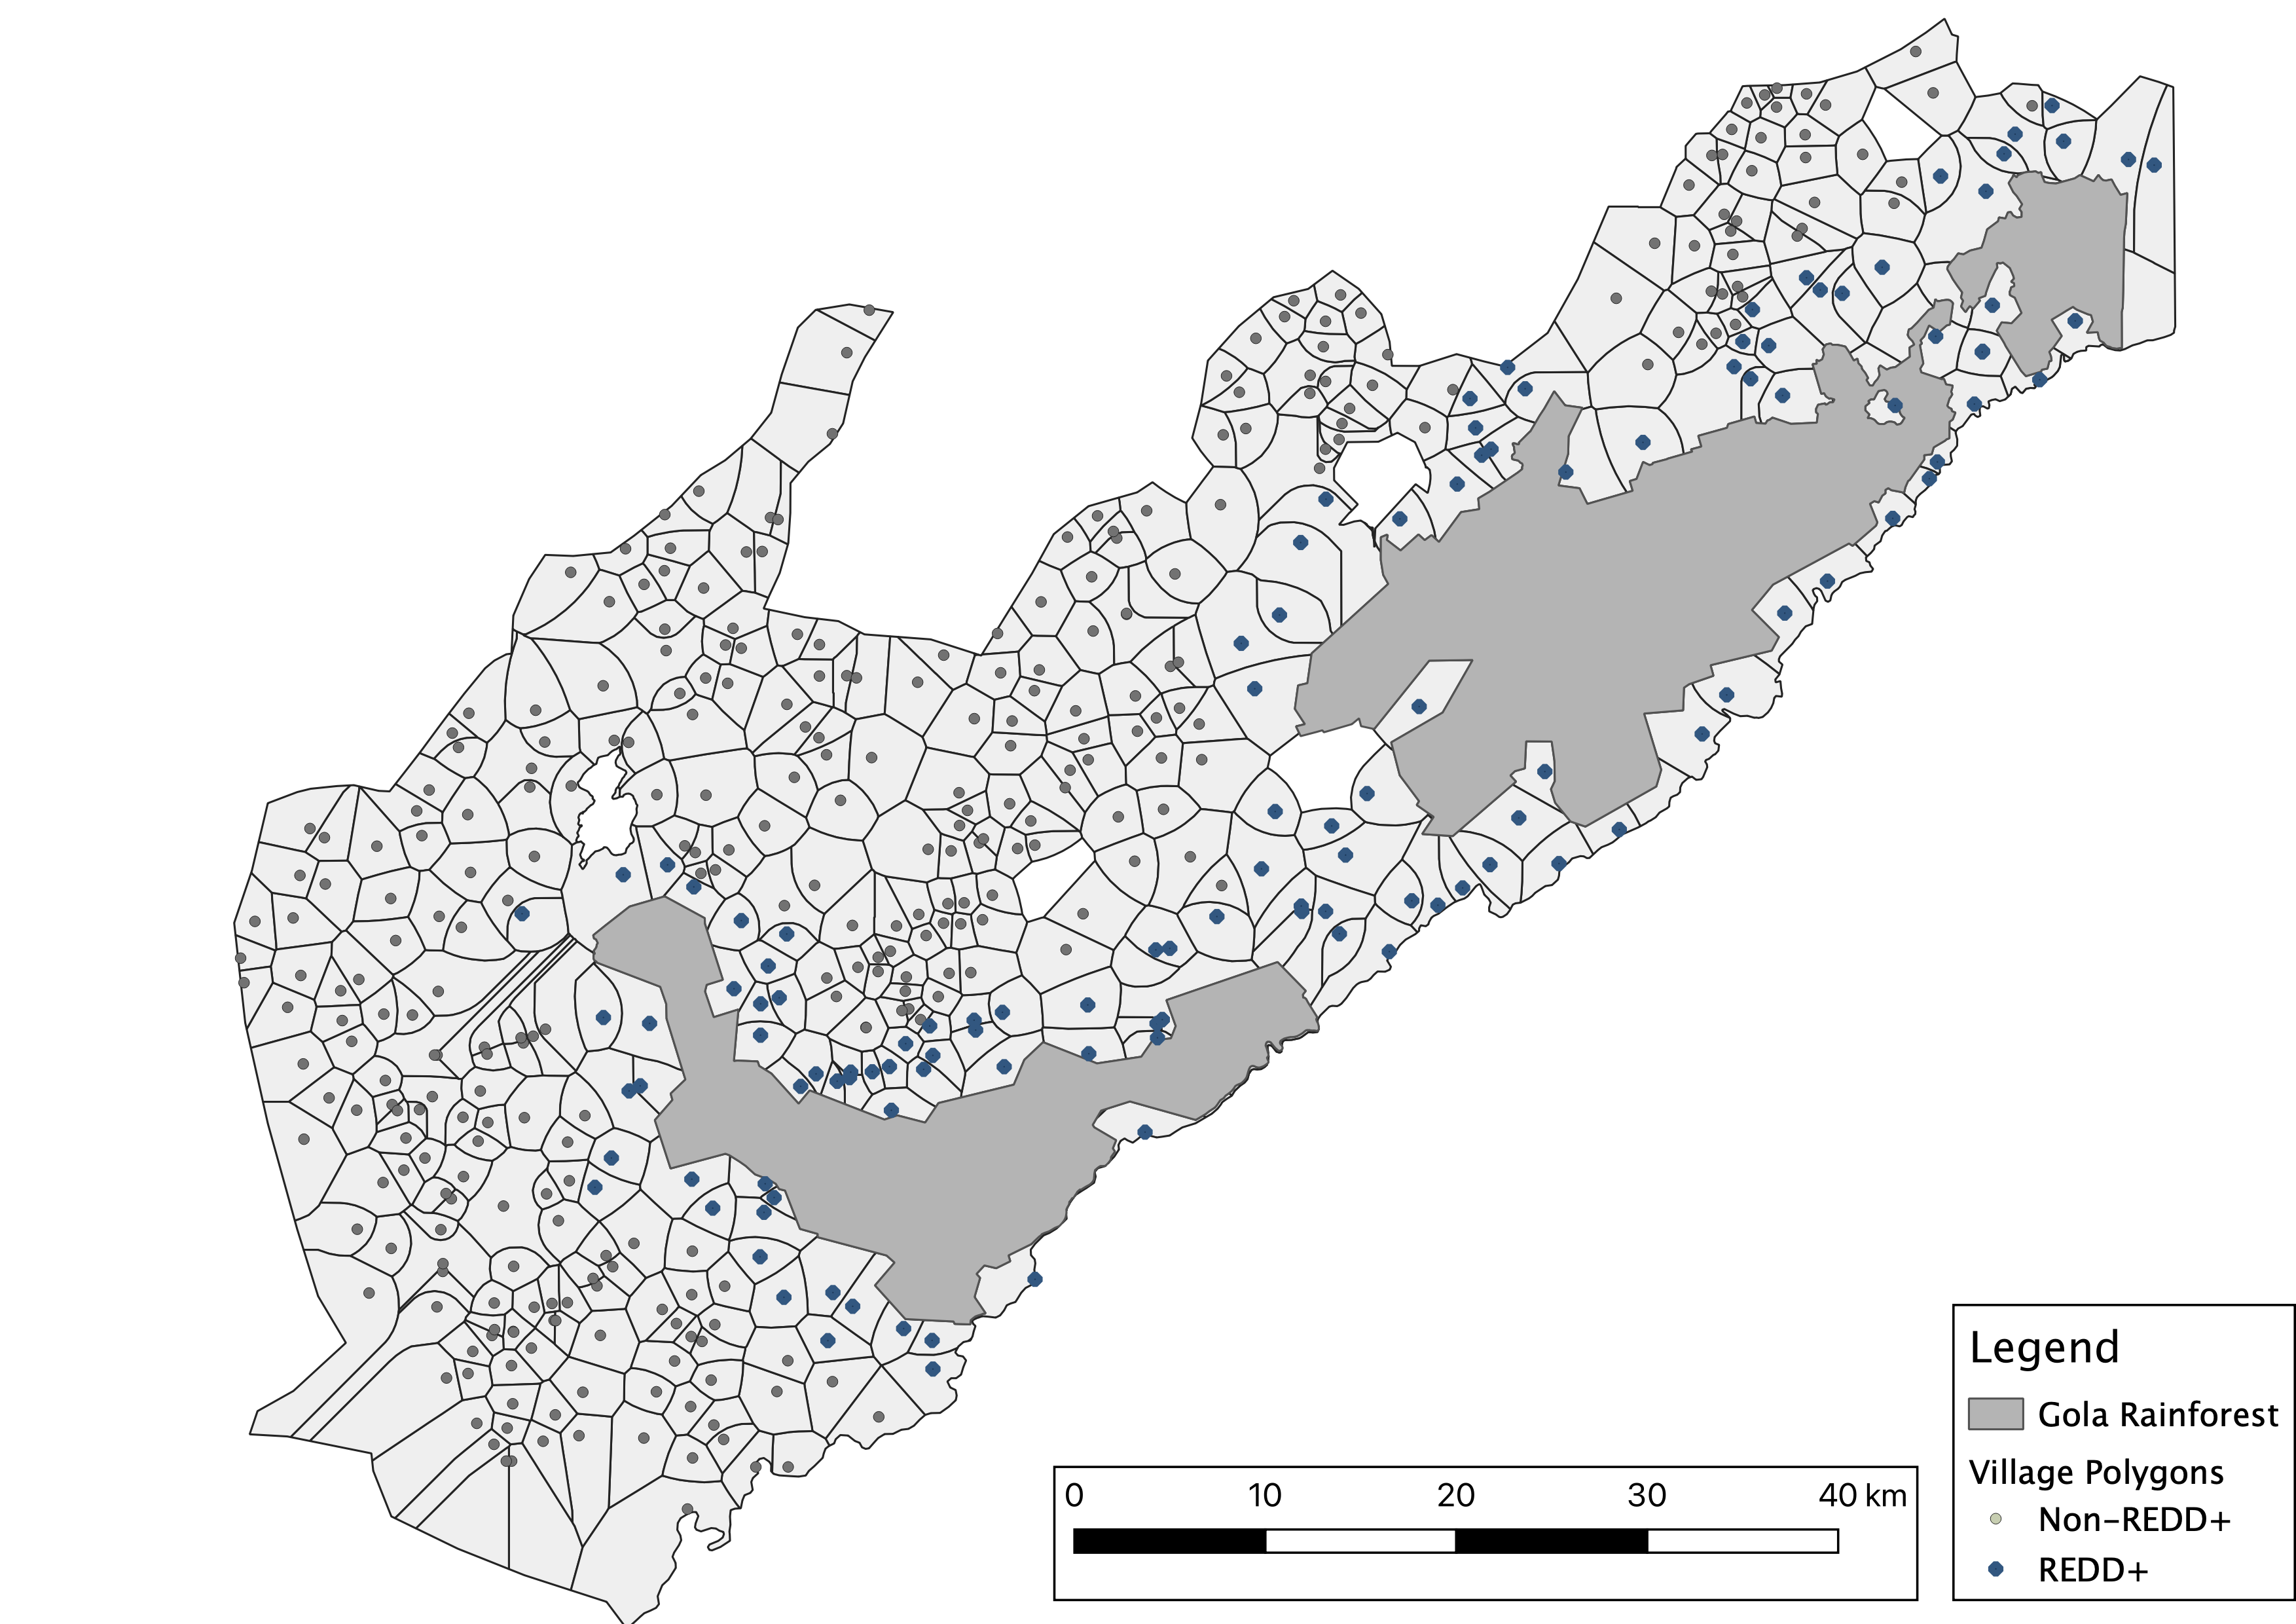
\includegraphics[width=0.9\linewidth]{3_maps/Village_polygons_greyscale} 

}

\caption{\textbf{Village polygons for satellite analysis.} This figure shows the village polygons used for the deforestation analysis. Polygons are estimated using the Voronoi method with weights based on village-estimates of the size obtained from Wilebore and Coomes (2016). If this estimate was not available (not all villages were surveyed), the polygon was not weighted. REDD+ villages are defined as villages that were eligible for the REDD+ programme. Non-REDD+ villages are villages that were not eligible for the REDD+ programme and lie outside the forest edge. There are a couple of polygons excluded because they are part of another protected area (Tiwai island) or leased land by companies (blank polygons in the map).}\label{fig:figPolygons}
\end{figure}

\begin{figure}[H]

{\centering 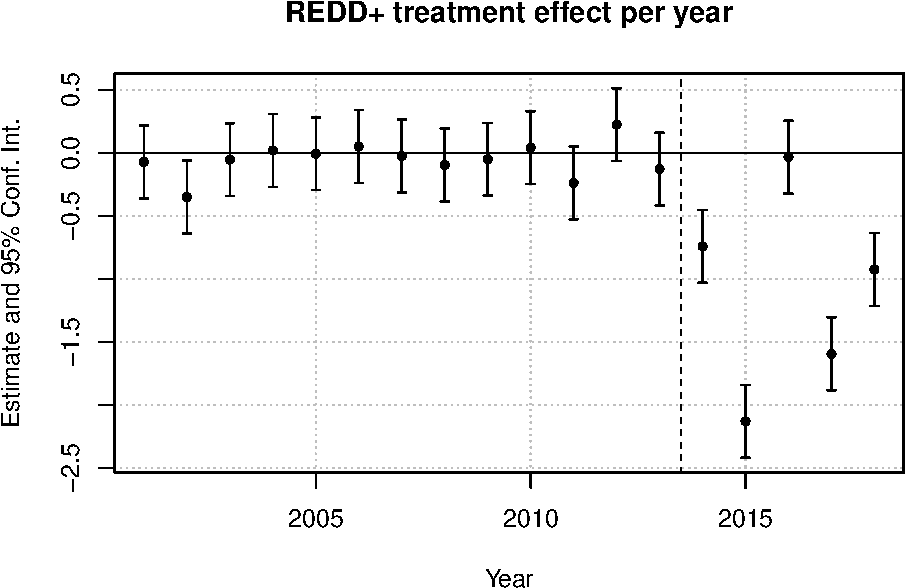
\includegraphics{paper_REDD_replication_files/figure-latex/figEventStudy-1} 

}

\caption{\textbf{Pre-treatment trends and treatment effect of REDD+ per year on forest loss} This graph shows year-specific treatment effect of REDD+ from 2001 to 2018 on forest loss and parallel pre-treatment trends. Sample includes all 454 REDD+ and non-REDD+ villages. The yearly treatment effects are estimated in an event study set-up using a fixed-effects OLS estimation. Data are represented as mean village-level treatment effects and error bars show 95 percent confidence intervals. The dashed line shows the start of REDD+. Source of data: Hansen 2013/UMD/Google/USGS/NASA.}\label{fig:figEventStudy}
\end{figure}

\hypertarget{survey-data-1}{%
\subsection*{Survey data}\label{survey-data-1}}
\addcontentsline{toc}{subsection}{Survey data}

This section provides more information about the survey data used to
evaluate the impact of REDD+ on economic wellbeing and conservation
attitudes. See a full description of the survey data collection in the
Methods section. In this section we describe our variables and compare
differences across REDD+ and non-REDD+ villages before the start of
program activities, using data from 2010 and 2014. Overall, differences
are small in magnitude and largely non-significant. For the method used
(difference-in-difference) level differences are not problematic, only
differences in trends are. Figure D2 shows a map of where survey data
was collected. Table D2 shows that for a range of covariates, of which
many are drivers of deforestation, REDD+ and non-REDD+ communities are
similar. Table D3 shows the differences in means in our outcomes from
survey data collected in 2010, comparing REDD+ and non-REDD+ villages.
Table D4 presents the same information for 2014. The differences are
small and unlikely to drive our main result. To further alleviate
concerns of baseline balance we also do an additional matching analysis,
using the covariates included in Table D2, our results are qualitatively
similar (see Supplementary Table F7). In Table D5, we explore parallel
trends with a pre-treatment trends analysis in which we run our
difference-in-difference model using 2010 and 2014 data. If trends prior
to treatment were parallel, we should see no significant 2014*REDD+
coefficients. As this is the case, we are confident that trends prior to
treatment were parallel which makes the parallel trends assumption more
likely to hold. Finally, Table D6 shows an attrition analysis for the
2014-2019 period. The dependent variable is whether a household attrited
in 2019. We see that participants with a high level of assets are less
likely to attrit. Importantly, there are no systematic differences in
the drivers of attrition between REDD+ and non-REDD+ villages.

\begin{figure}[H]

{\centering 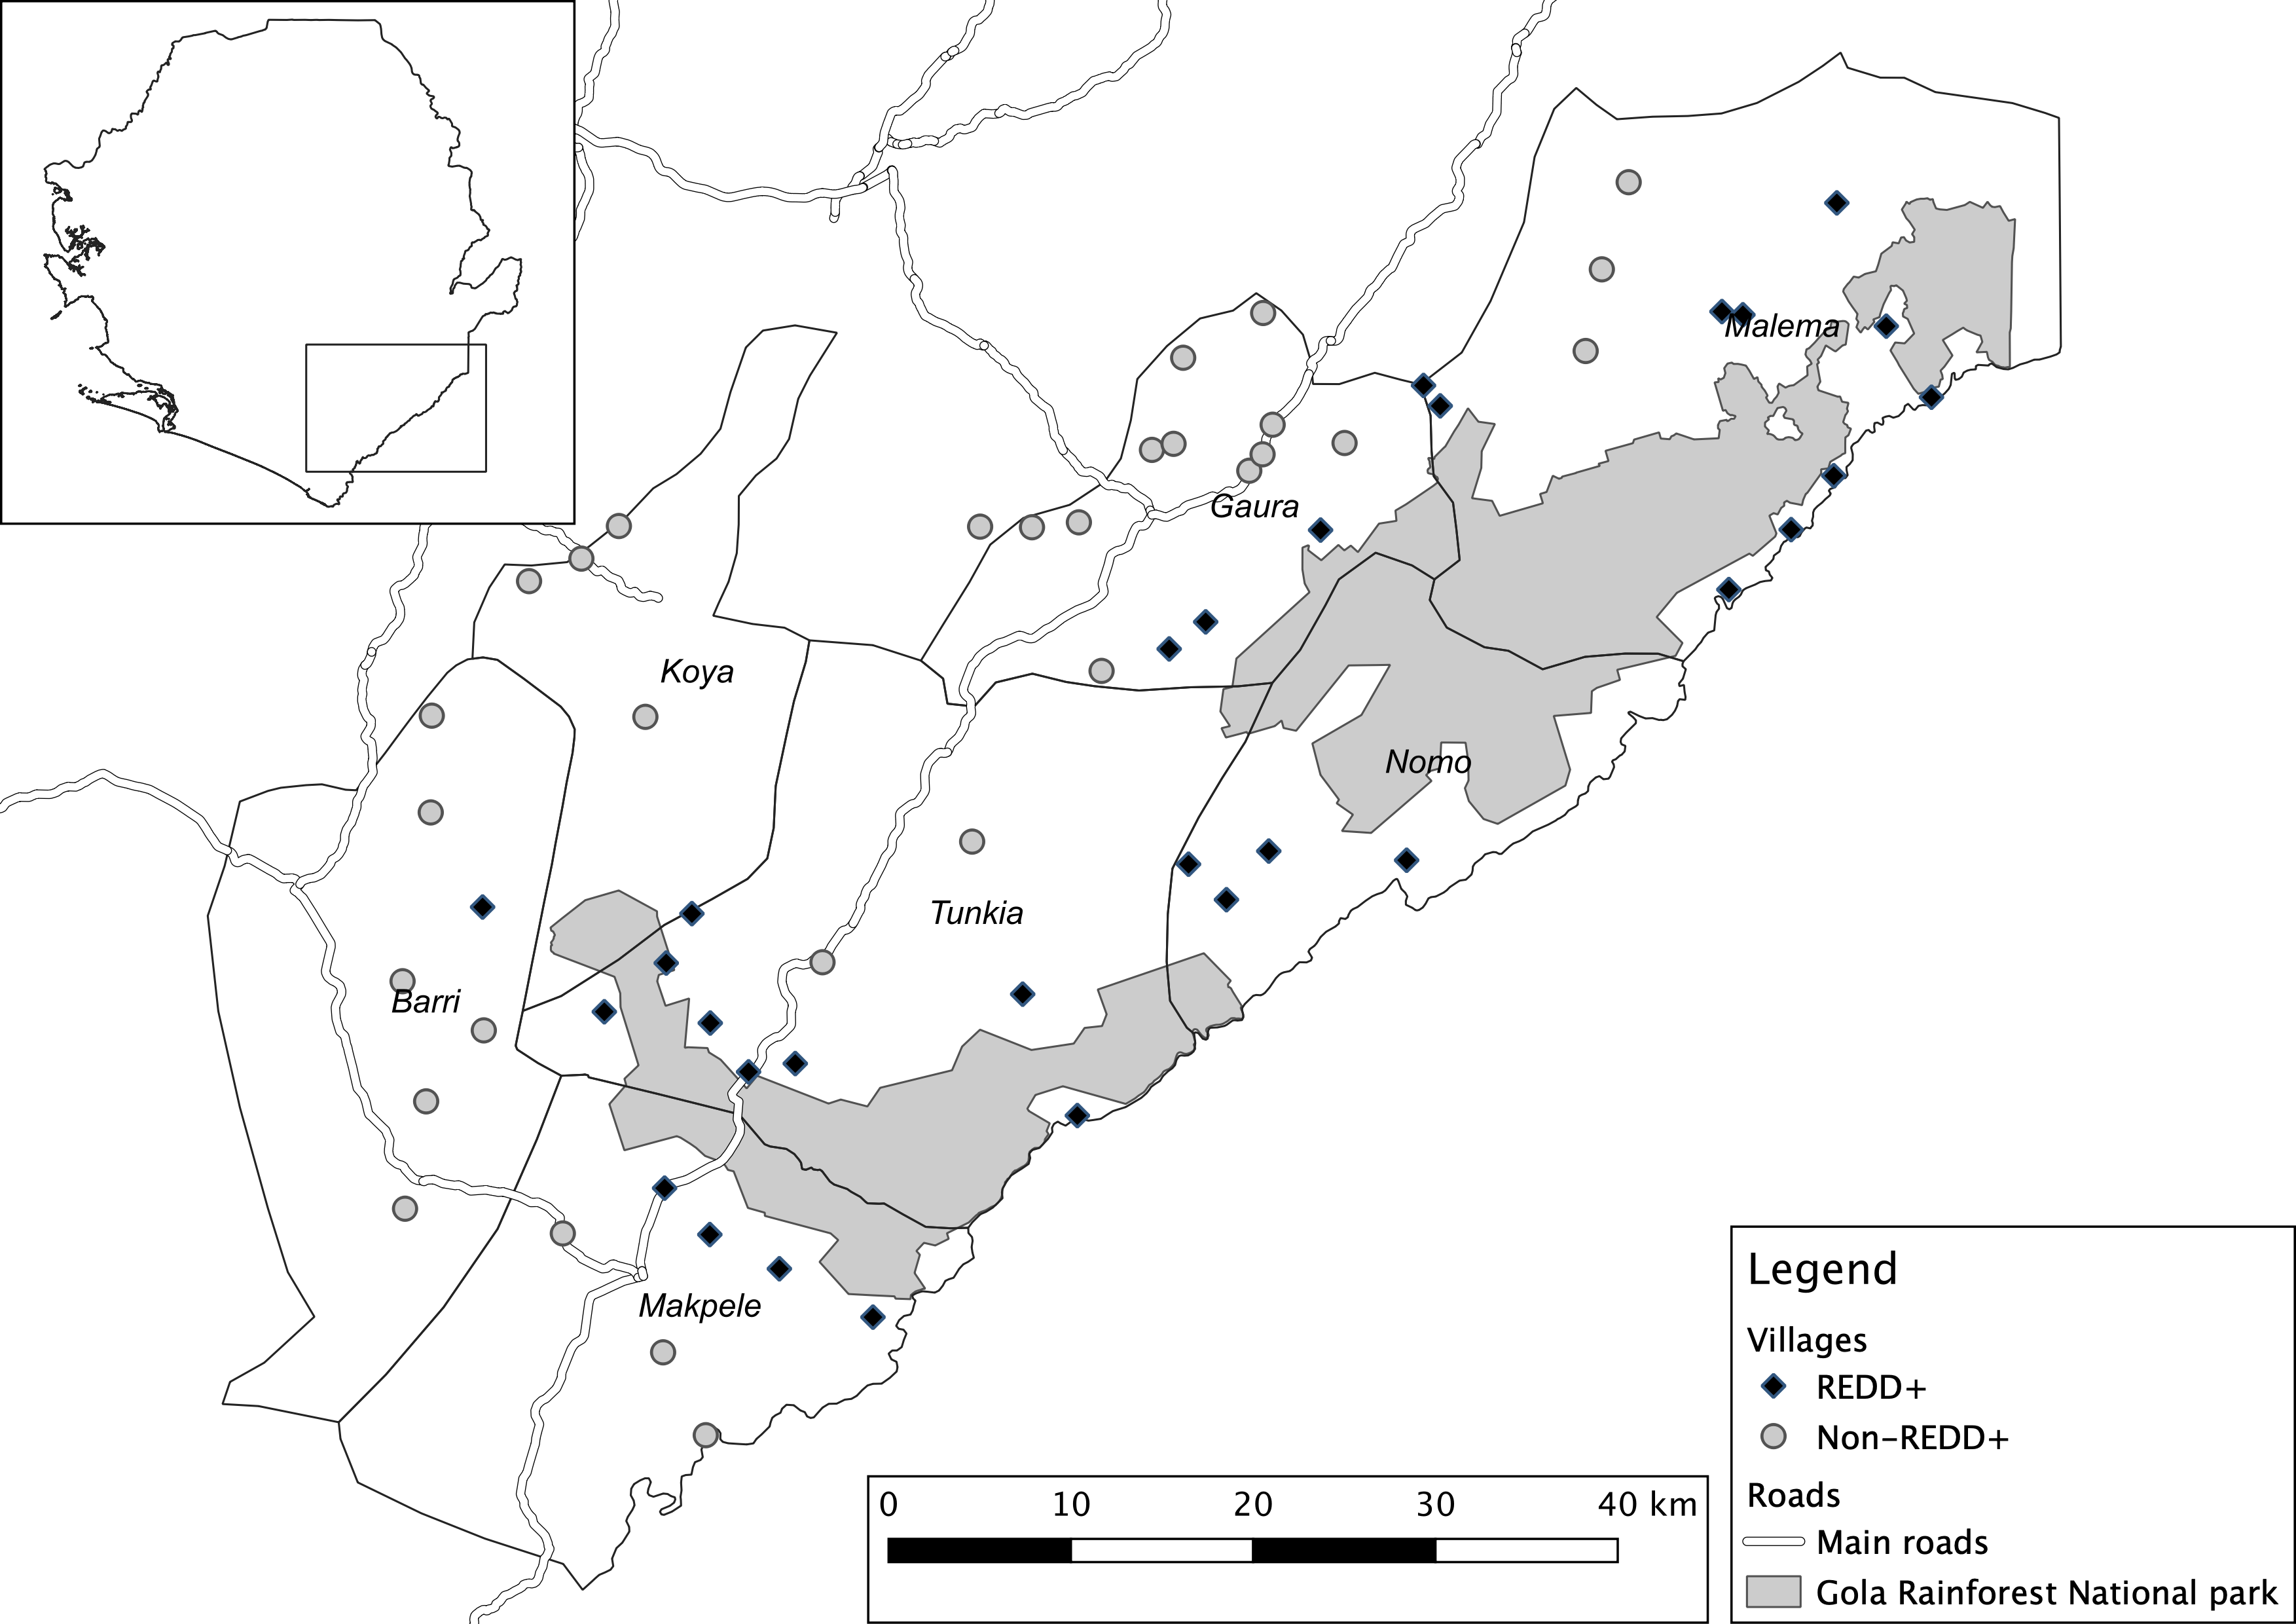
\includegraphics[width=0.9\linewidth]{3_maps/REDD_Map_greyscale} 

}

\caption{\textbf{Survey sample.} This figure shows the sample for the survey data. 30 REDD+ villages, ie those eligible for REDD+ benefits were randomly selected. These communities all lie within a 4 km band around the National Park. We also selected 30 non-REDD+ villages which were randomly selected from villages 4-25 km from the National Park boundary. The sampling was stratified by regional quadrants to ensure representation of villages between the GRNP boundary and the border with Liberia. One of the REDD+ villages was removed from the sample as it no longer existed bringing our full sample down to 59.}\label{fig:figSample}
\end{figure}

\begin{table}[!h]

\caption{\label{tab:tabSumstatsCov}\textbf{Difference in means in covariates}}
\centering
\begin{threeparttable}
\begin{tabular}[t]{lllllllc}
\toprule
\multicolumn{1}{c}{ } & \multicolumn{3}{c}{non-REDD+} & \multicolumn{3}{c}{REDD+} & \multicolumn{1}{c}{ } \\
\cmidrule(l{3pt}r{3pt}){2-4} \cmidrule(l{3pt}r{3pt}){5-7}
\textbf{Variable} & \textbf{N} & \textbf{Mean} & \textbf{SD} & \textbf{N} & \textbf{Mean} & \textbf{SD} & \textbf{Difference}\\
\midrule
\addlinespace[0.3em]
\multicolumn{8}{l}{\textbf{Village-level covariates}}\\
\hspace{1em}Village (polygon) size (ha) & 328 & 5833.310 & 4286.875 & 126 & 7106.675 & 3989.180 & 1273.365***\\
\hspace{1em}Average slope (degrees) & 328 & 3.812 & 1.516 & 126 & 4.771 & 1.521 & 0.959\\
\hspace{1em}Time to health care facility (min) & 328 & 15.454 & 11.982 & 126 & 51.133 & 53.108 & 35.678\\
\hspace{1em}Time to GRNP (min) & 328 & 43.160 & 25.593 & 126 & 31.557 & 21.003 & -11.603\\
\hspace{1em}Human settlement (\% of area) & 328 & 0.006 & 0.018 & 126 & 0.001 & 0.002 & -0.005\\
\hspace{1em}Forested (\% of area) & 328 & 31.899 & 20.946 & 126 & 66.853 & 24.103 & 34.954\\
\addlinespace[0.3em]
\multicolumn{8}{l}{\textbf{Household-level covariates}}\\
\hspace{1em}Household head age & 364 & 0.000 & 0.000 & 296 & 0.000 & 0.000 & 0.074*\\
\hspace{1em}Household size & 364 & 44.549 & 14.875 & 296 & 47.666 & 16.838 & 2.087\\
\hspace{1em}Female headed household (=1) & 364 & 8.827 & 4.733 & 296 & 8.209 & 3.892 & -0.553\\
\hspace{1em}Education: none (=1) & 364 & 0.203 & 0.402 & 296 & 0.230 & 0.421 & 0.038\\
\hspace{1em}Education: primary (=1) & 364 & 0.385 & 0.487 & 296 & 0.432 & 0.495 & 0.048\\
\hspace{1em}Education: secondary (=1) & 364 & 0.110 & 0.313 & 296 & 0.095 & 0.293 & -0.001\\
\hspace{1em}Cocoa farmer (=1) & 364 & 0.115 & 0.319 & 296 & 0.071 & 0.257 & -0.048**\\
\hspace{1em}Plantation size (acres) & 364 & 0.681 & 0.466 & 296 & 0.679 & 0.467 & -0.01\\
\hspace{1em}Upland farm size (acres) & 364 & 6.339 & 8.182 & 296 & 5.792 & 5.721 & -0.478\\
\hspace{1em}Swampland farm size (acres) & 364 & 1.602 & 3.084 & 296 & 1.700 & 4.014 & 0.159\\
\bottomrule
\end{tabular}
\begin{tablenotes}
\item \textit{Note: } 
\item Household-level covariates are from the 2014 survey wave. N is the number of observations, SD is the standard deviation. Difference gives the difference in means. P-values are calculated using a difference-in-means two-sided t-test, clustered for household-level indicators, where * p < 0.10, ** p < 0.05, *** p < 0.01.
\end{tablenotes}
\end{threeparttable}
\end{table}

\begin{table}[!h]

\caption{\label{tab:tabSumstats2010}\textbf{Difference in means in 2010 outcomes}}
\centering
\begin{threeparttable}
\begin{tabular}[t]{lllllllc}
\toprule
\multicolumn{1}{c}{ } & \multicolumn{3}{c}{non-REDD+} & \multicolumn{3}{c}{REDD+} & \multicolumn{1}{c}{ } \\
\cmidrule(l{3pt}r{3pt}){2-4} \cmidrule(l{3pt}r{3pt}){5-7}
\textbf{Variable} & \textbf{N} & \textbf{Mean} & \textbf{SD} & \textbf{N} & \textbf{Mean} & \textbf{SD} & \textbf{Difference}\\
\midrule
Total income (Leones, IHS) & 370 & 6.693 & 1.846 & 286 & 6.412 & 1.675 & -0.281\\
Monthly consumption expenditure (Leones, IHS) & 370 & 5.001 & 1.379 & 286 & 4.815 & 1.569 & -0.186\\
Yearly irregular expenditure (Leones, IHS) & 370 & 7.329 & 0.957 & 286 & 7.102 & 0.916 & -0.226*\\
Durable loan size, (Leones, IHS) & 370 & 0.632 & 1.838 & 286 & 0.396 & 1.440 & -0.236\\
Sustainable farming practices (0-4) & 331 & 0.272 & 0.852 & 240 & 0.533 & 1.131 & 0.261**\\
Yearly income farm wages (Leones, IHS) & 370 & 2.139 & 2.211 & 286 & 2.168 & 2.099 & 0.029\\
Yearly income from NTFPs (Leones, IHS) & 370 & 1.563 & 2.150 & 286 & 0.988 & 1.907 & -0.575**\\
Labour access index (0-3) & 364 & 1.391 & 0.921 & 285 & 1.276 & 0.879 & -0.115\\
\bottomrule
\end{tabular}
\begin{tablenotes}
\item \textit{Note: } 
\item N is the number of observations, SD is the standard deviation. Difference gives the difference in means. IHS indicates that the variable is transformed using an inverse hyperbolic sine function. P-values are calculated using a clustered difference-in-means two-sided t-test where * p < 0.10, ** p < 0.05, *** p < 0.01.
\end{tablenotes}
\end{threeparttable}
\end{table}

\begin{table}[!h]

\caption{\label{tab:tabSumstats}\textbf{Difference in means in 2014 outcomes}}
\centering
\begin{threeparttable}
\begin{tabular}[t]{lllllllc}
\toprule
\multicolumn{1}{c}{ } & \multicolumn{3}{c}{non-REDD+} & \multicolumn{3}{c}{REDD+} & \multicolumn{1}{c}{ } \\
\cmidrule(l{3pt}r{3pt}){2-4} \cmidrule(l{3pt}r{3pt}){5-7}
\textbf{Variable} & \textbf{N} & \textbf{Mean} & \textbf{SD} & \textbf{N} & \textbf{Mean} & \textbf{SD} & \textbf{Difference}\\
\midrule
Total income (Leones, IHS) & 364 & 6.498 & 2.418 & 296 & 6.199 & 2.230 & -0.299\\
Monthly consumption expenditure (Leones, IHS) & 364 & 6.015 & 1.473 & 296 & 6.008 & 1.549 & -0.008\\
Yearly irregular expenditure (Leones, IHS) & 364 & 7.406 & 0.972 & 296 & 7.289 & 1.010 & -0.116\\
Durable loan size, (Leones, IHS) & 364 & 0.302 & 1.542 & 296 & 0.112 & 0.866 & -0.191\\
Resilience (=1) & 352 & 0.696 & 0.461 & 287 & 0.753 & 0.432 & 0.057\\
Conservation attitudes (4-20) & 353 & 17.040 & 2.740 & 290 & 17.424 & 2.500 & 0.384\\
Awareness of conservation norms (0-5) & 320 & 3.075 & 0.287 & 263 & 3.209 & 0.477 & 0.134***\\
Sustainable farming practices (0-4) & 363 & 0.388 & 0.911 & 296 & 0.470 & 0.894 & 0.081\\
Human wildlife conflict (0-3) & 361 & -2.363 & 1.027 & 288 & -2.580 & 0.852 & -0.217**\\
Yearly income farm wages (Leones, IHS) & 363 & 0.043 & 1.020 & 295 & 0.028 & 0.983 & -0.015\\
Yearly income from NTFPs (Leones, IHS) & 364 & 0.636 & 1.650 & 296 & 0.385 & 1.202 & -0.251\\
Labour access index (0-3) & 341 & 1.254 & 1.005 & 283 & 1.279 & 0.995 & 0.025\\
Cocoa harvests (kg, IHS) & 364 & 1.090 & 2.076 & 296 & 0.836 & 1.895 & -0.254\\
\bottomrule
\end{tabular}
\begin{tablenotes}
\item \textit{Note: } 
\item N is the number of observations, SD is the standard deviation. Difference gives the difference in means. IHS indicates that the variable is transformed using an inverse hyperbolic sine function. P-values are calculated using a clustered difference-in-means two-sided t-test where * p < 0.10, ** p < 0.05, *** p < 0.01.
\end{tablenotes}
\end{threeparttable}
\end{table}

\begin{landscape}

\begin{table}[h]
\caption{\textbf{Parallel trends 2010-2014 for available outcomes}}
\begin{center}
\begin{tabular}{l c c c c c c c c}
\hline
 & Economic wellbeing & Income & Assets & Durable loan & Sustainable farming & Labour access & Income farm wages & Income NTFP \\
\hline
2014*REDD+ & $0.216$        & $0.230$       & $0.146$        & $0.088$        & $-0.157$     & $0.219$   & $0.088$        & $0.221$        \\
           & $(0.152)$      & $(0.284)$     & $(0.126)$      & $(0.096)$      & $(0.158)$    & $(0.189)$ & $(0.124)$      & $(0.145)$      \\
2014       & $0.291^{**}$   & $0.333$       & $0.663^{***}$  & $-0.229^{***}$ & $0.120$      & $-0.208$  & $-0.397^{***}$ & $-0.470^{***}$ \\
           & $(0.117)$      & $(0.209)$     & $(0.066)$      & $(0.080)$      & $(0.122)$    & $(0.148)$ & $(0.101)$      & $(0.097)$      \\
REDD+      & $-0.370^{***}$ & $-0.298^{**}$ & $-0.350^{***}$ & $-0.128$       & $0.307^{**}$ & $-0.125$  & $0.013$        & $-0.268^{**}$  \\
           & $(0.109)$      & $(0.122)$     & $(0.121)$      & $(0.084)$      & $(0.120)$    & $(0.108)$ & $(0.112)$      & $(0.123)$      \\
Constant   & $0.000$        & $0.000$       & $0.000$        & $-0.000$       & $0.000$      & $-0.000$  & $-0.000$       & $0.000$        \\
           & $(0.076)$      & $(0.089)$     & $(0.087)$      & $(0.055)$      & $(0.081)$    & $(0.088)$ & $(0.089)$      & $(0.082)$      \\
\hline
Years      & 2              & 2             & 2              & 2              & 2            & 2         & 2              & 2              \\
Num. obs.  & $1312$         & $1312$        & $1312$         & $1312$         & $1225$       & $1262$    & $1310$         & $1312$         \\
N Clusters & $56$           & $56$          & $56$           & $56$           & $56$         & $56$      & $56$           & $56$           \\
\hline
\multicolumn{9}{l}{\scriptsize{\parbox{1.05\linewidth}{\vspace{2pt}$^{***}p<0.01$; $^{**}p<0.05$; $^{*}p<0.1$ based on two-sided t-test.\\
                      Difference-in-difference analysis using OLS regressions to test for parallel trends between 2010 and 2014. 2014*REDD+ is the coefficient of interest, testing for differences in pre-treatment trends. The economic wellbeing family outcome is a summary index (average of z-scores) of an income index, an assets index, a durable loan size measure. The income index is a summary index (average of z-scores) of total householdincome, monthly consumption expenditure and yearly durable expenditure. Assets is the sum of all assetsowned. Durable loan size is the amount borrowed for durable investments. Sustainable farming practices measures the number of practices usedby a household. Labour access index is an index of three farm labour access variables (upland rice, wetlandrice, and plantation) indicating to what extent there is access to labour. Income farm wages is a continuous variable (IHS transformed) measuring the yearly household income from farm wages. Income NTFP is a continuous variable (IHS transformed) measuring the yearly income from Non-Timber Forest Products collection. All outcomes are standardised and centred on control group at baseline and coefficients should be interpreted as standard deviation changes. Standard errors are clustered at the village level. Robust standard errors in parentheses.}}}
\end{tabular}
\label{table:coefficients}
\end{center}
\end{table}
\end{landscape}

\begin{table}[h!]
\caption{\textbf{Attrition analysis: primary outcomes}}
\begin{center}
\begin{tabular}{l c}
\hline
 & Attrition \\
\hline
Income                             & $0.014$        \\
                                   & $(0.023)$      \\
Assets                             & $-0.065^{***}$ \\
                                   & $(0.022)$      \\
Durable loan size                  & $0.004$        \\
                                   & $(0.018)$      \\
Resilience                         & $-0.013$       \\
                                   & $(0.022)$      \\
Conservation attitudes             & $-0.003$       \\
                                   & $(0.019)$      \\
Awareness of conservation norms    & $0.021$        \\
                                   & $(0.024)$      \\
Sustainable farming practices      & $-0.003$       \\
                                   & $(0.021)$      \\
Human wildlife conflict perception & $0.022$        \\
                                   & $(0.019)$      \\
REDD+                              & $0.079^{*}$    \\
                                   & $(0.043)$      \\
*Income                            & $-0.035$       \\
                                   & $(0.032)$      \\
*Assets                            & $0.036$        \\
                                   & $(0.029)$      \\
*Durable loan size                 & $0.026$        \\
                                   & $(0.028)$      \\
*Resilience                        & $0.031$        \\
                                   & $(0.035)$      \\
*Conservation attitudes            & $-0.003$       \\
                                   & $(0.038)$      \\
*Conservation norms                & $-0.049$       \\
                                   & $(0.029)$      \\
*Sustainable farming               & $-0.000$       \\
                                   & $(0.027)$      \\
*Human wildlife conflict           & $-0.018$       \\
                                   & $(0.034)$      \\
Constant                           & $0.151^{***}$  \\
                                   & $(0.024)$      \\
\hline
Num. obs.                          & $817$          \\
N Clusters                         & $59$           \\
\hline
\multicolumn{2}{l}{\scriptsize{\parbox{.5\linewidth}{\vspace{2pt}$^{***}p<0.01$; $^{**}p<0.05$; $^{*}p<0.1$ based on two-sided t-test.\\ Attrition analysis with data from 2014. The dependent variable is whether a household dropped out in 2019. All variables starting with * are interactions with the treatment-variable (REDD+). Missing values are imputed at the own group-mean. All outcomes are standardized and centered on control group mean and coefficients should be interpreted as standard deviation changes. Standard errors are clustered at the village level. Robust standard errors in parentheses.}}}
\end{tabular}
\label{table:coefficients}
\end{center}
\end{table}

\setcounter{table}{0}  
\renewcommand{\thetable}{E\arabic{table}}
\setcounter{figure}{0} 
\renewcommand{\thefigure}{E\arabic{figure}}

\clearpage

\hypertarget{supplementary-information-e-additional-results}{%
\section*{Supplementary Information E: Additional
results}\label{supplementary-information-e-additional-results}}
\addcontentsline{toc}{section}{Supplementary Information E: Additional
results}

In this section we provide additional tables with results for outcomes
as specified in our pre-analysis plan. All models run in this section
are difference-in-difference models as described in the Methods section.
Table E1 shows the results for our satellite outcome forest loss and
includes the distinction between primary and secondary forest loss.
Forest loss is mainly driven by changed to secondary forests. In Tables
E2-E5, we estimate differences for each indicator included in the
economic wellbeing and conservation attitude index used in Table 1.
Table E2 and E3 present standardized results and Tables E4 and E5
unstandardised results for all outcomes. Table E6 and E7 show the
results for pre-specified secondary outcomes. Finally, Table E8 shows an
analysis where we test whether households moved out of villages
(measured by number of households living in a village) because of the
REDD+ programme. In none of the results is the interaction term is
significant.

\begin{table}[h]
\caption{\textbf{The impact of REDD+ on primary and secondary forest loss (satellite data)}}
\begin{center}
\begin{tabular}{l c c c}
\hline
 & Forest loss & Primary forest loss & Secondary forest loss \\
\hline
Post*REDD+       & $-1.032^{***}$ & $0.058$       & $-0.577^{**}$ \\
                 & $(0.114)$      & $(0.039)$     & $(0.230)$     \\
Post             & $3.314^{***}$  & $0.050^{***}$ & $0.455^{***}$ \\
                 & $(0.066)$      & $(0.014)$     & $(0.110)$     \\
REDD+            & $-0.052$       & $0.212^{***}$ & $-0.157$      \\
                 & $(0.033)$      & $(0.031)$     & $(0.211)$     \\
Constant         & $0.740^{***}$  & $0.082^{***}$ & $2.527^{***}$ \\
                 & $(0.017)$      & $(0.011)$     & $(0.096)$     \\
\hline
Years            & $18$           & $6$           & $6$           \\
Village polygons & $454$          & $434$         & $434$         \\
Num. obs.        & $8172$         & $2604$        & $2604$        \\
\hline
\multicolumn{4}{l}{\scriptsize{\parbox{.7\linewidth}{\vspace{2pt}$^{***}p<0.01$; $^{**}p<0.05$; $^{*}p<0.1$ based on two-sided t-test.\\
       Difference-in-difference analysis using OLS regressions for forest loss (satellite data). Post*REDD+ is the project impact coefficient. Forest loss is the percentage loss of forest (primary and secondary). Primary forest loss is loss of old growth forest and secondary forest loss measures conversion of fallow to production agriculture. Both are classified through extensive ground measurements, which were done in 2013. The number of observations is therefore lower for these two outcomes, as data ranges from 2013-2018. Robust standard errors in parentheses.}}}
\end{tabular}
\label{table:coefficients}
\end{center}
\end{table}

\begin{table}[h]
\caption{\textbf{The impact of REDD+ on livelihood indicators (survey data)}}
\begin{center}
\begin{tabular}{l c c c c c}
\hline
 & Economic wellbeing & Income & Assets & Durable loan & Resilience \\
\hline
Post*REDD+ & $0.022$      & $0.017$   & $-0.039$      & $0.176$   & $-0.171$      \\
           & $(0.132)$    & $(0.143)$ & $(0.094)$     & $(0.107)$ & $(0.149)$     \\
Post       & $0.222^{**}$ & $-0.020$  & $-0.120^{*}$  & $-0.029$  & $0.644^{***}$ \\
           & $(0.103)$    & $(0.111)$ & $(0.068)$     & $(0.079)$ & $(0.133)$     \\
REDD+      & $-0.144$     & $-0.090$  & $-0.275^{**}$ & $-0.124$  & $0.186$       \\
           & $(0.118)$    & $(0.122)$ & $(0.104)$     & $(0.078)$ & $(0.152)$     \\
Constant   & $0.000$      & $-0.000$  & $-0.000$      & $0.000$   & $0.000$       \\
           & $(0.089)$    & $(0.085)$ & $(0.079)$     & $(0.068)$ & $(0.136)$     \\
\hline
N panel    & $660$        & $660$     & $660$         & $660$     & $416$         \\
Num. obs.  & $1320$       & $1320$    & $1320$        & $1320$    & $832$         \\
N Clusters & $59$         & $59$      & $59$          & $59$      & $58$          \\
\hline
\multicolumn{6}{l}{\scriptsize{\parbox{.8\linewidth}{\vspace{2pt}$^{***}p<0.01$; $^{**}p<0.05$; $^{*}p<0.1$ based on two-sided t-test.\\
       Difference-in-difference analysis using OLS regression for livelihood outcomes. Post*REDD+ is the project impact coefficient. The economic wellbeing family outcome is a summary index (average of z-scores) of an income index, an assets index, a durable loan size measure, and a measure for resilience. The income index is a summary index (average of z-scores) of total household income, monthly consumption expenditure and yearly durable expenditure. Assets is the sum of all assets owned. Durable loan size is the amount borrowed for durable investments. Resilience is a conditional dummy (on whether the household suffered from an emergency) of whether households were able to deal with an emergency. All outcomes are standardised and centred on control group at baseline and these coefficients should be interpreted as standard deviation changes. Standard errors are clustered at the village level. Robust standard errors in parentheses.}}}
\end{tabular}
\label{table:coefficients}
\end{center}
\end{table}

\begin{table}[h]
\caption{\textbf{The impact of REDD+ on conservation norms indicators (survey data)}}
\begin{center}
\begin{tabular}{l c c c c c}
\hline
 & Conservation family & Attitudes & Knowledge & Sustainable farming & HWC \\
\hline
Post*REDD+ & $-0.017$  & $-0.300$       & $0.287$       & $0.113$   & $-0.040$      \\
           & $(0.218)$ & $(0.206)$      & $(0.250)$     & $(0.157)$ & $(0.135)$     \\
Post       & $-0.226$  & $-0.822^{***}$ & $0.210$       & $-0.012$  & $0.124^{*}$   \\
           & $(0.138)$ & $(0.113)$      & $(0.170)$     & $(0.119)$ & $(0.067)$     \\
REDD+      & $0.176$   & $0.132$        & $0.427^{***}$ & $0.102$   & $-0.204^{**}$ \\
           & $(0.130)$ & $(0.132)$      & $(0.154)$     & $(0.112)$ & $(0.096)$     \\
Constant   & $-0.000$  & $-0.000$       & $-0.000$      & $-0.000$  & $0.000$       \\
           & $(0.076)$ & $(0.091)$      & $(0.087)$     & $(0.090)$ & $(0.074)$     \\
\hline
N panel    & $660$     & $597$          & $518$         & $647$     & $635$         \\
Num. obs.  & $1320$    & $1194$         & $1036$        & $1294$    & $1270$        \\
N Clusters & $59$      & $59$           & $59$          & $59$      & $59$          \\
\hline
\multicolumn{6}{l}{\scriptsize{\parbox{.9\linewidth}{\vspace{2pt}$^{***}p<0.01$; $^{**}p<0.05$; $^{*}p<0.1$ based on two-sided t-test.\\
       Difference-in-difference analysis using OLS regression for conservation norms outcomes. Post*REDD+ is the project impact coefficient. The conservation family outcome is a summary index (average of z-scores) of a conservation attitudes index, an awareness of conservation norms index, the number of sustainable farming practices practiced, and an index for human wildlife conflict perception (HWC). Conservation attitudes is an index of agreement with pro-conservation statements. Awareness of conservation norms is an index of knowledge on rules regarding conservation. Sustainable farming practices measures the number of practices used by a household. HWC measures how big of a problem crop-raiding is. All outcomes are standardised and centred on control group at baseline and these coefficients should be interpreted as standard deviation changes. Standard errors are clustered at the village level. Robust standard errors in parentheses.}}}
\end{tabular}
\label{table:coefficients}
\end{center}
\end{table}

\begin{table}[h]
\caption{\textbf{The impact of REDD+ on primary outcomes (unstandardised)}}
\begin{center}
\begin{tabular}{l c c c c c}
\hline
 & Durable loan & Attitudes & Knowledge & Sustainable farming & HWC \\
\hline
Post*REDD+ & $0.272$       & $-0.829$       & $0.086$       & $0.103$       & $-0.041$       \\
           & $(0.165)$     & $(0.570)$      & $(0.075)$     & $(0.143)$     & $(0.137)$      \\
Post       & $-0.045$      & $-2.276^{***}$ & $0.063$       & $-0.011$      & $0.125^{*}$    \\
           & $(0.122)$     & $(0.313)$      & $(0.051)$     & $(0.108)$     & $(0.068)$      \\
REDD+      & $-0.191$      & $0.364$        & $0.128^{***}$ & $0.093$       & $-0.206^{**}$  \\
           & $(0.120)$     & $(0.367)$      & $(0.046)$     & $(0.102)$     & $(0.098)$      \\
Constant   & $0.302^{***}$ & $17.003^{***}$ & $3.081^{***}$ & $0.380^{***}$ & $-2.382^{***}$ \\
           & $(0.105)$     & $(0.252)$      & $(0.026)$     & $(0.082)$     & $(0.074)$      \\
\hline
N panel    & $660$         & $597$          & $518$         & $647$         & $635$          \\
Num. obs.  & $1320$        & $1194$         & $1036$        & $1294$        & $1270$         \\
N Clusters & $59$          & $59$           & $59$          & $59$          & $59$           \\
\hline
\multicolumn{6}{l}{\scriptsize{\parbox{.88\linewidth}{\vspace{2pt}$^{***}p<0.01$; $^{**}p<0.05$; $^{*}p<0.1$ based on two-sided t-test.\\
       Difference-in-difference analysis using OLS regression for all unstandardised primary (non-index) outcomes. Post*REDD+ is the project impact coefficient. Durable loan size is the amount borrowed for durable investments. Conservation attitudes is an index of agreement with pro-conservation statements. Awareness of conservation norms is an index of knowledge on rules regarding conservation. Sustainable farming practices measures the number of practices used by a household. HWC measures how big of a problem crop-raiding is. Standard errors are clustered at the village level. Robust standard errors in parentheses.}}}
\end{tabular}
\label{table:coefficients}
\end{center}
\end{table}

\begin{table}[h]
\caption{\textbf{The impact of REDD+ on plausible mechanisms (unstandardised)}}
\begin{center}
\begin{tabular}{l c c c c}
\hline
 & Labour acces index & Income farm wages & Income NTFP & Cocoa harvest \\
\hline
Post*REDD+ & $-0.534^{**}$ & $0.435^{*}$   & $0.567^{**}$  & $0.406$        \\
           & $(0.252)$     & $(0.233)$     & $(0.252)$     & $(0.269)$      \\
Post       & $0.358^{**}$  & $0.082$       & $0.034$       & $-1.067^{***}$ \\
           & $(0.157)$     & $(0.181)$     & $(0.175)$     & $(0.213)$      \\
REDD+      & $0.118$       & $-0.031$      & $-0.251$      & $-0.254$       \\
           & $(0.130)$     & $(0.211)$     & $(0.166)$     & $(0.262)$      \\
Constant   & $1.181^{***}$ & $1.307^{***}$ & $0.636^{***}$ & $1.090^{***}$  \\
           & $(0.089)$     & $(0.139)$     & $(0.144)$     & $(0.212)$      \\
\hline
Years      & 2             & 2             & 2             & 2              \\
Villages   & $59$          & $59$          & $59$          & $59$           \\
Num. obs.  & $1150$        & $1228$        & $1320$        & $1320$         \\
\hline
\multicolumn{5}{l}{\scriptsize{\parbox{.9\linewidth}{\vspace{2pt}$^{***}p<0.01$; $^{**}p<0.05$; $^{*}p<0.1$ based on two-sided t-test.\\
       Difference-in-difference analysis using OLS regressions for unstandardised mechanisms. Post*REDD+ is the project impact coefficient. Labour access index is an index of three farm labour access variables (upland rice, wetland rice, and plantation) indicating to what extent there is access to labour. Income farm wages is a continuous variable (IHS transformed) measuring the yearly household income from farm wages. Income NTFP is a continuous variable (IHS transformed) measuring the yearly income from Non-Timber Forest Products collection. Standard errors are clustered at the village level. Robust standard errors in parentheses.}}}
\end{tabular}
\label{table:coefficients}
\end{center}
\end{table}

\begin{landscape}

\begin{table}[h]
\caption{\textbf{The impact of REDD+ on secondary outcomes}}
\begin{center}
\begin{tabular}{l c c c c c c c}
\hline
 & Farm Income & Cocoa Income & Off Farm Inc & Upland Size & Wetland Size & Plantation Size & Health \\
\hline
Post*REDD+ & $0.220$       & $0.078$      & $0.099$   & $0.014$   & $-0.118$     & $-0.006$  & $-0.055$       \\
           & $(0.168)$     & $(0.152)$    & $(0.176)$ & $(0.267)$ & $(0.234)$    & $(0.172)$ & $(0.131)$      \\
Post       & $0.326^{***}$ & $0.278^{*}$  & $-0.115$  & $0.178$   & $0.333^{**}$ & $-0.064$  & $-0.630^{***}$ \\
           & $(0.109)$     & $(0.135)$    & $(0.148)$ & $(0.169)$ & $(0.156)$    & $(0.152)$ & $(0.074)$      \\
REDD+      & $-0.276^{**}$ & $-0.233^{*}$ & $-0.126$  & $0.176$   & $0.036$      & $-0.017$  & $-0.060$       \\
           & $(0.135)$     & $(0.127)$    & $(0.127)$ & $(0.123)$ & $(0.121)$    & $(0.096)$ & $(0.117)$      \\
Constant   & $0.000$       & $0.000$      & $-0.000$  & $-0.000$  & $0.000$      & $-0.000$  & $-0.000$       \\
           & $(0.092)$     & $(0.093)$    & $(0.108)$ & $(0.069)$ & $(0.100)$    & $(0.077)$ & $(0.068)$      \\
\hline
N panel    & $660$         & $660$        & $660$     & $607$     & $600$        & $616$     & $660$          \\
Num. obs.  & $1320$        & $1320$       & $1320$    & $1214$    & $1200$       & $1232$    & $1320$         \\
N Clusters & $59$          & $59$         & $59$      & $59$      & $59$         & $59$      & $59$           \\
\hline
\multicolumn{8}{l}{\scriptsize{\parbox{.84\linewidth}{\vspace{2pt}$^{***}p<0.01$; $^{**}p<0.05$; $^{*}p<0.1$ based on two-sided t-test.\\
       Difference-in-difference analysis using OLS regression for secondary outcomes. Post*REDD+ is the project impact coefficient. Farm income is the total income from crop sales. Cocoa income is the total income from cocoa sales. Cocoa harvests is the total cocoa production. Off farm income is the total income from off farm activities. Upland farm size is the total size of the upland (rice) farm. Wetland size is the total size of the wetland (rice) farm. Plantation size is the total size of the plantation area. Health is the number of household members with malaria and/or blood in stool and/or diarrhoea in the previous month. All outcomes are standardised and centred on control group at baseline and coefficients should be interpreted as standard deviation changes. Standard errors are clustered at the village level. Robust standard errors in parentheses.}}}
\end{tabular}
\label{table:coefficients}
\end{center}
\end{table}

\begin{table}[h]
\caption{\textbf{The impact of REDD+ on secondary outcomes (unstandardised)}}
\begin{center}
\begin{tabular}{l c c c c c c c}
\hline
 & Farm Income & Cocoa Income & Off Farm Inc & Upland Size & Wetland Size & Plantation Size & Health \\
\hline
Post*REDD+ & $0.737$       & $0.226$       & $0.248$       & $0.014$       & $-0.100$      & $-0.007$      & $-0.267$       \\
           & $(0.562)$     & $(0.441)$     & $(0.443)$     & $(0.261)$     & $(0.198)$     & $(0.193)$     & $(0.640)$      \\
Post       & $1.092^{***}$ & $0.803^{*}$   & $-0.289$      & $0.174$       & $0.281^{**}$  & $-0.072$      & $-3.074^{***}$ \\
           & $(0.364)$     & $(0.392)$     & $(0.373)$     & $(0.166)$     & $(0.131)$     & $(0.170)$     & $(0.363)$      \\
REDD+      & $-0.925^{**}$ & $-0.674^{*}$  & $-0.318$      & $0.173$       & $0.031$       & $-0.019$      & $-0.294$       \\
           & $(0.453)$     & $(0.369)$     & $(0.319)$     & $(0.120)$     & $(0.102)$     & $(0.108)$     & $(0.570)$      \\
Constant   & $3.734^{***}$ & $1.691^{***}$ & $5.847^{***}$ & $1.612^{***}$ & $0.842^{***}$ & $2.028^{***}$ & $6.220^{***}$  \\
           & $(0.307)$     & $(0.269)$     & $(0.271)$     & $(0.068)$     & $(0.084)$     & $(0.087)$     & $(0.334)$      \\
\hline
N panel    & $660$         & $660$         & $660$         & $607$         & $600$         & $616$         & $660$          \\
Num. obs.  & $1320$        & $1320$        & $1320$        & $1214$        & $1200$        & $1232$        & $1320$         \\
N Clusters & $59$          & $59$          & $59$          & $59$          & $59$          & $59$          & $59$           \\
\hline
\multicolumn{8}{l}{\scriptsize{\parbox{.84\linewidth}{\vspace{2pt}$^{***}p<0.01$; $^{**}p<0.05$; $^{*}p<0.1$ based on two-sided t-test.\\
       Difference-in-difference analysis using OLS regression for unstandardised secondary outcomes. Post*REDD+ is the project impact coefficient.Farm income is the total income from crop sales. Cocoa income is the total income from cocoa sales. Cocoa harvests is the total cocoa production. Off farm income is the total income from off farm activities. Upland farm size is the total size of the upland (rice) farm. Wetland size is the total size of the wetland (rice) farm. Plantation size is the total size of the plantation area. All these outcomes are transformed using the inverse hyperbolic sine transformation. Health is the number of household members with malaria and/or blood in stool and/or diarrhoea in the previous month. Standard errors are clustered at the village level. Robust standard errors in parentheses.}}}
\end{tabular}
\label{table:coefficients}
\end{center}
\end{table}
\end{landscape}

\begin{table}[h]
\caption{\textbf{The impact of REDD+ on village size}}
\begin{center}
\begin{tabular}{l c}
\hline
 & Village size \\
\hline
Post*REDD+ & $0.270$        \\
           & $(0.361)$      \\
Post       & $0.011$        \\
           & $(0.254)$      \\
REDD+      & $-0.784^{***}$ \\
           & $(0.248)$      \\
Constant   & $0.000$        \\
           & $(0.183)$      \\
\hline
Years      & 2              \\
Villages   & 58             \\
Num. obs.  & $116$          \\
\hline
\multicolumn{2}{l}{\scriptsize{\parbox{.5\linewidth}{\vspace{2pt}$^{***}p<0.01$; $^{**}p<0.05$; $^{*}p<0.1$ based on two-sided t-test.\\
       Difference-in-difference analysis using OLS regression for number of households at the community level. We treat this variable as a proxy for migration. The outcome is standardised and centred on control group at baseline and the coefficients should be interpreted as standard deviation changes.}}}
\end{tabular}
\label{table:coefficients}
\end{center}
\end{table}

\setcounter{table}{0}  
\renewcommand{\thetable}{F\arabic{table}}
\setcounter{figure}{0} 
\renewcommand{\thefigure}{F\arabic{figure}}
\clearpage

\hypertarget{supplementary-information-f-robustness-analysis}{%
\section*{Supplementary Information F: Robustness
analysis}\label{supplementary-information-f-robustness-analysis}}
\addcontentsline{toc}{section}{Supplementary Information F: Robustness
analysis}

\hypertarget{satellite-data-1}{%
\subsection{Satellite data}\label{satellite-data-1}}

This section shows the results of several robustness checks for the main
deforestation result of the REDD+ programme presented in Figure 3 and
Table 1. First, in Table F1, we compare forest loss as measured by
Global Forest Change (GFC) dataset by Hansen et al.~(2013) with the
recently released Tropical Moist Forest dataset (TMF) by Vancutsem et
al.~(2021)\textsuperscript{45}. Even though the coefficient of interest
is slightly smaller using the TMF dataset (-0.759 compared to -1.032 for
GFC), it shows a similar \textasciitilde27\% reduction in deforestation
in the treatment area after the start of the REDD+ programme.

Upon closer visual inspection, the evolution of forest loss according to
TMF is quite different from GFC. In Panel B of Figure F1, it appears
that prior to Landsat 8 (launched in 2013), trends in deforestation were
not as parallel as they are for GFC. Furthermore, in 2013 the difference
between REDD+ and non-REDD+ villages is much larger. From 2016 onwards,
deforestation reduces dramatically in both REDD+ and non-REDD+ villages.
Looking at other national park buffer zones in Sierra Leone, we see the
same puzzling pattern.

\begin{table}[h]
\caption{\textbf{Robustness forest loss: GFC and TMF data}}
\begin{center}
\begin{tabular}{l c c}
\hline
 & GFC (original) & TMF \\
\hline
Post*REDD+       & $-1.032^{***}$ & $-0.759^{***}$ \\
                 & $(0.114)$      & $(0.145)$      \\
Post             & $3.314^{***}$  & $2.847^{***}$  \\
                 & $(0.066)$      & $(0.087)$      \\
REDD+            & $-0.052$       & $-0.357^{***}$ \\
                 & $(0.033)$      & $(0.042)$      \\
Constant         & $0.740^{***}$  & $0.894^{***}$  \\
                 & $(0.017)$      & $(0.026)$      \\
\hline
Years            & $18$           & $18$           \\
Village polygons & $454$          & $454$          \\
Num. obs.        & $8172$         & $8172$         \\
\hline
\multicolumn{3}{l}{\scriptsize{\parbox{.5\linewidth}{\vspace{2pt}$^{***}p<0.01$; $^{**}p<0.05$; $^{*}p<0.1$ based on two-sided t-test.\\
       Difference-in-difference analysis using OLS regressions for forest loss (satellite data). Forest loss is the percentage loss of forest. The first column shows the original regression with forest loss data from 2001-2018 from the Global Forest Change dataset (Hansen et al. 2013). The second column shows the same model with data from 2001-2018 from the Tropical Moist Forest dataset (Vancutsem et al. 2021). Robust standard errors in parentheses.}}}
\end{tabular}
\label{table:coefficients}
\end{center}
\end{table}

Some of the differences between GFC and TMF forest loss rates can be
explained by differences in how deforestation is measured. First,
identification of deforestation in the TMF dataset is based on
single-date deforestation events. That is, a single Landsat picture (on
one specific day) that shows forest loss could show up as deforestation
in the TMF dataset. Essentially, this means that TMF can pick up
deforestation events up to a year before GFC. This could explain the
large differences between REDD+ and non-REDD+ villages in 2013.
Additionally, the algorithm used by TMF is different from GFC, as it
focuses on tropical moist forests, while GFC focuses on all forested
areas worldwide. One possible result of this, noted by Vancutsem et al
(2021) themselves as well as by Tyukavina et al (2015), is that GFC
might underestimate deforestation, especially for
Africa\textsuperscript{45,53}. We see the same pattern in our analyses.
However, as our main interest is in changes over time, level differences
are less relevant.

\begin{figure}[H]

{\centering 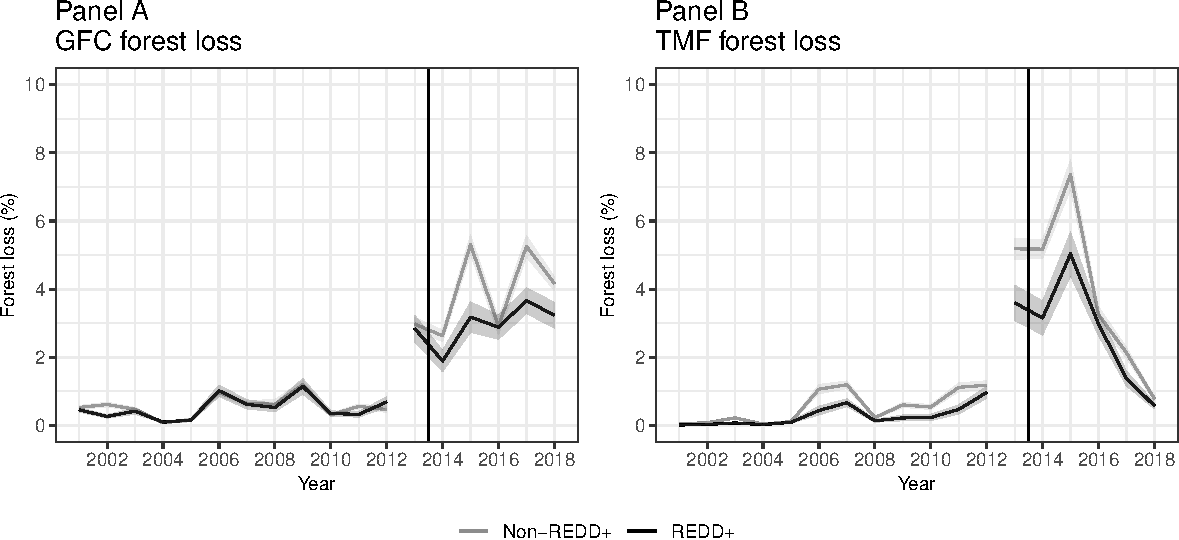
\includegraphics[width=6in]{paper_REDD_replication_files/figure-latex/figForestlossGFC_TMF-1} 

}

\caption{\textbf{Total forest loss in REDD+ and non-REDD+ villages for GFC and TMF data} This graph shows total forest loss from 2001 to 2018 in REDD+ versus non-REDD+ villages for the Global Forest Change (GFC) and Tropical Moist Forest (TMF) data. The village polygons are estimated using population weighted Voronoi estimations. Data are represented as mean village-level values and shaded areas in the graph denote 95 percent confidence intervals. The vertical black line indicates the start of REDD+. The break in the lines in 2013 denotes the launch of a new satellite (Landsat 8) resulting in more precise measures of forest loss. Source of data: Hansen 2013/Vancutsem 2021/UMD/Google/USGS/NASA.}\label{fig:figForestlossGFC_TMF}
\end{figure}

\begin{table}[!h]

\caption{\label{tab:tabBins}\textbf{Satellite matching covariates and CEM-cutoff points}}
\centering
\begin{threeparttable}
\begin{tabular}[t]{>{\raggedright\arraybackslash}p{20em}l}
\toprule
\textbf{Variable} & \textbf{Cutoff points}\\
\midrule
Village (polygon) size (ha) & 200,1000\\
Average slope (degrees) & 6\\
Time to health care facility (min) & 60,180\\
Time to GRNP (min) & 10,50\\
Human settlement (\% of area) & 0.005,0.05\\
Forested (\% of area) & 10,50,75\\
\bottomrule
\end{tabular}
\begin{tablenotes}
\item \textit{Note: } 
\item This table shows the matching variables used for propensity score matching (PSM) and coarsened exact matching (CEM). The cutoff points used for CEM are provided in Column 2. 
\end{tablenotes}
\end{threeparttable}
\end{table}

As an additional robustness check, we employ matching methods in
combination with our difference-in-difference analysis. We use
propensity score matching (PSM), with nearest neighbour method and
coarsened exact matching (CEM) for both the GFC dataset and the TMF
dataset. The covariates used to match treated communities to control
communities and the cutoff points used for CEM are shown in Table F2
(refer to Supplementary D2, for descriptive statistics of these
covariates). For this analysis, presented in Table F3, the outcome we
use is the difference in deforestation between the period prior to REDD+
(2001-2013) and after REDD+ (2014-2018). Across all models, we see a
significant reduction in forest loss in the REDD+ ranging from -0.618\%
to -1.297\% per year, very similar to the main estimates presented in
Column 1.

\begin{table}[h]
\caption{\textbf{Robustness forest loss: matching and dif-in-dif for GFC and TMF data}}
\begin{center}
\begin{tabular}{l c c c c c c}
\hline
 & \multicolumn{2}{c}{Original} & \multicolumn{2}{c}{PSM} & \multicolumn{2}{c}{CEM} \\
\cline{2-3} \cline{4-5} \cline{6-7}
 & GFC & TMF & GFC & TMF & GFC & TMF \\
\hline
REDD+     & $-1.032^{***}$ & $-0.759^{***}$ & $-1.037^{***}$ & $-1.297^{***}$ & $-0.837^{***}$ & $-0.618^{***}$ \\
          & $(0.139)$      & $(0.136)$      & $(0.164)$      & $(0.163)$      & $(0.225)$      & $(0.219)$      \\
Constant  & $3.314^{***}$  & $2.847^{***}$  & $3.319^{***}$  & $3.385^{***}$  & $3.603^{***}$  & $3.195^{***}$  \\
          & $(0.066)$      & $(0.071)$      & $(0.109)$      & $(0.114)$      & $(0.109)$      & $(0.142)$      \\
\hline
Num. obs. & $454$          & $454$          & $252$          & $252$          & $217$          & $217$          \\
\hline
\multicolumn{7}{l}{\scriptsize{\parbox{.80\linewidth}{\vspace{2pt}$^{***}p<0.01$; $^{**}p<0.05$; $^{*}p<0.1$ based on two-sided t-test.\\
                      Robustness analysis using different methods for Global Forest Watch (GFC) and Tropical Moist Forest (TMF) data. REDD+ is the project impact coefficient. The Original columns show a standard OLS regression. The PSM columns show results of propensity score matching, using the nearest neighbour approach, combined with OLS. Covariates used for matching are: the polygon (village) size, the average slope, average walking time to nearest health care facility (a proxy for market access), average walking time to the GRNP border, the proportion of the area with human settlements and the proportion of the area forested. The CEM columns show the results for the coarsened exact matching function using the same covariates. All outcomes measure the difference in the percentage of forest loss between the pre-REDD+ (2001-2013) and post-REDD+ period (2014-2018). Robust standard errors in parentheses.}}}
\end{tabular}
\label{table:coefficients}
\end{center}
\end{table}

We then use alternative definitions of the treatment and control group
samples to address the concern that observed differences between REDD+
communities and control communities are confounded by proximity to the
park. We run three different models in which we use alternative distance
boundaries of our treatment and control villages and present them in
Table F4 (Figure F2 shows a map with the different assignments). In
Column 2 of Table F4, we restrict the control group to communities
within 8km from the park, dropping the villages furthest from the park
from the control group. This hardly changes the coefficient (by 0.06
percentage points). In Column 3 we do a falsification check and drop all
treated communities, thus comparing communities in the buffer zone from
4-8 km to control communities further away. The effect completely
disappears. In Column 4 we drop all communities that lie within 1.6 km
(1 mile) of the park. These villages were defined as Forest Edge
Communities by the GRNP before the start of the REDD+ programme and
received assistance in the pre-REDD+ period (See Supplementary
Information C for details). Here, the effect of REDD+ is smaller (0.741
vs 1.031 percentage points), suggesting that prior activities may have a
long-lasting effect on reducing deforestation in the area. Regardless,
the REDD+ programme still reduces deforestation by 0.74 percentage
points in the rest of the REDD+ area.

\begin{figure}[H]

{\centering 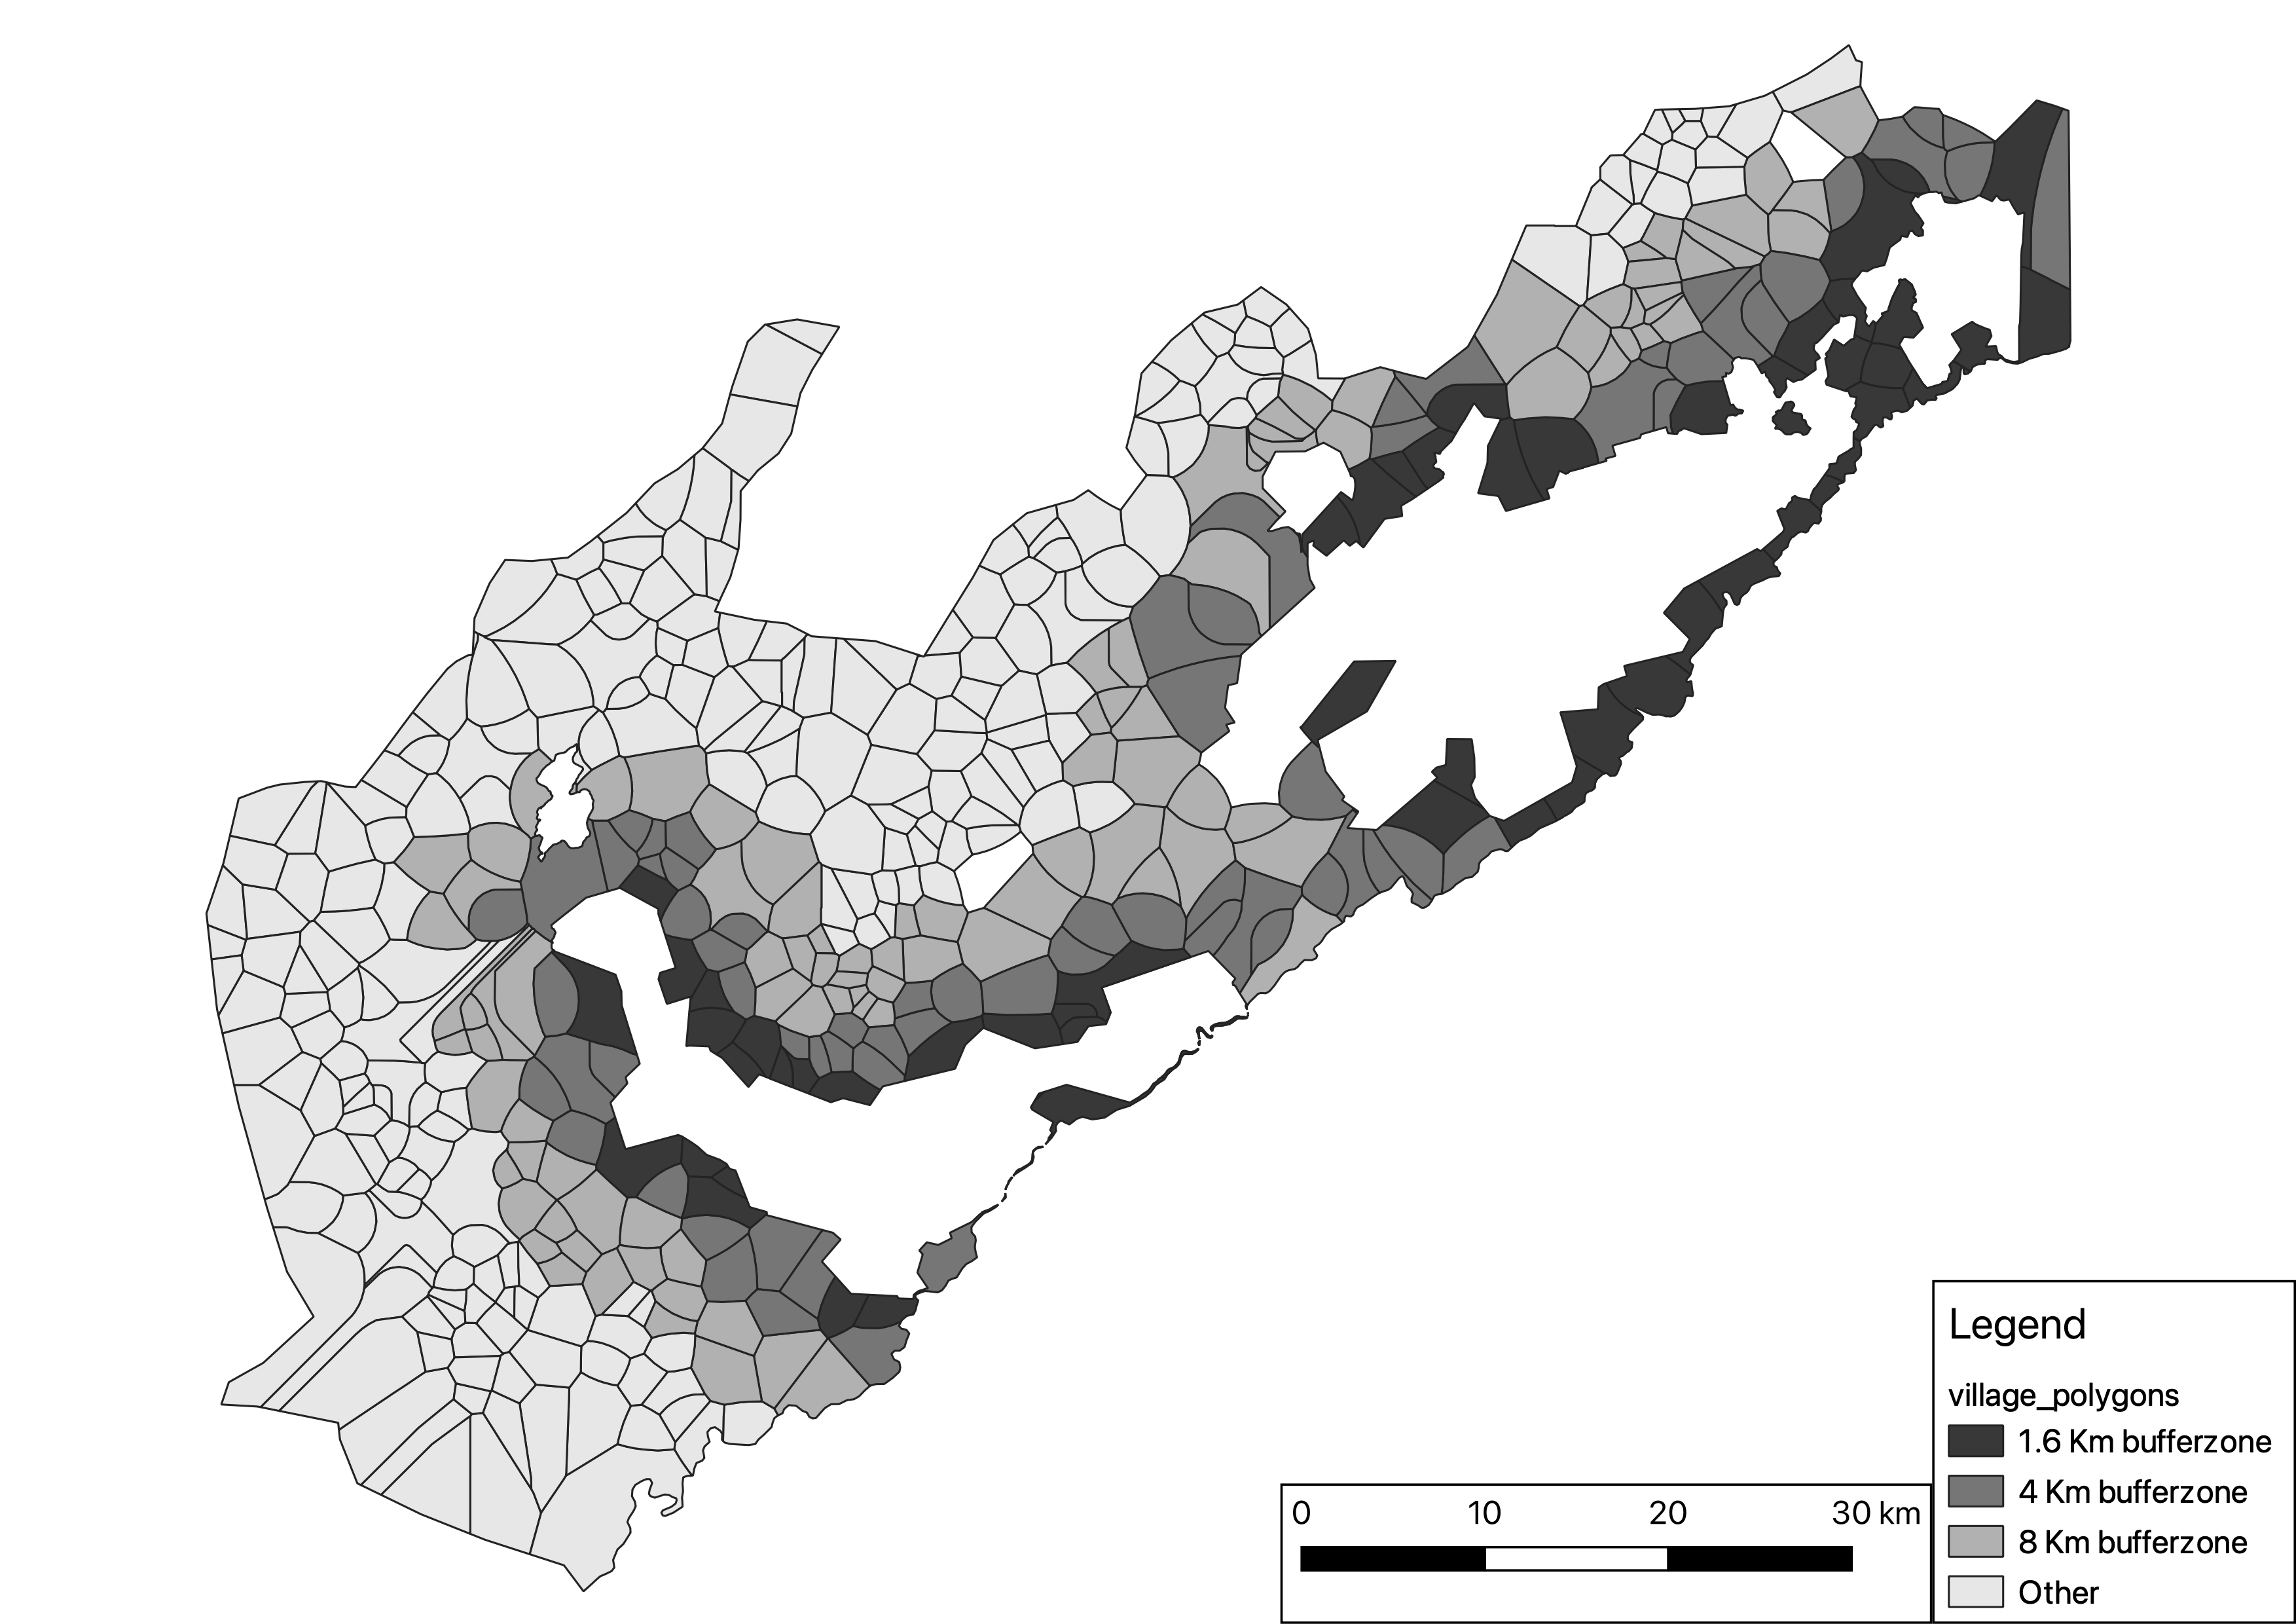
\includegraphics[width=0.9\linewidth]{3_maps/village_polygons_alt_1mile} 

}

\caption{\textbf{1.6 km, 4km and 8km buffer zone for robustness analysis.} This figure shows the village polygons used for robustness checks for the results on forest loss. Polygons are obtained from Wilebore and Coomes (2016). The figure shows the eligible REDD+ villages in the 4km buffer zone. The 1.6 km buffer zone shows villages that are 1 mile away from the forest - note that this is determined by the distance to the actual location of the village and not the distance to the village lands (polygon). The 8 km buffer zone band shows the 8km buffer zone that we use for the roustness tests below. There are a couple of polygons excluded because they are part of another protected area (Tiwai island) or leased land by companies (blank polygons).}\label{fig:figPolygonsRobust}
\end{figure}

\begin{table}[h!]
\caption{\textbf{Robustness forest loss: alternative treatment and control assignments}}
\begin{center}
\begin{tabular}{l c c c c}
\hline
 & Original & Control = 4-8km & 0-4km dropped & 0-1.6km dropped \\
\hline
Post*REDD+ & $-1.032^{***}$ & $-0.971^{***}$ &               & $-0.741^{***}$ \\
           & $(0.114)$      & $(0.147)$      &               & $(0.140)$      \\
Post*8km   &                &                & $-0.090$      &                \\
           &                &                & $(0.140)$     &                \\
Post       & $3.314^{***}$  & $3.253^{***}$  & $3.343^{***}$ & $3.314^{***}$  \\
           & $(0.066)$      & $(0.114)$      & $(0.080)$     & $(0.066)$      \\
REDD+      & $-0.052$       & $-0.123^{***}$ &               & $0.004$        \\
           & $(0.033)$      & $(0.043)$      &               & $(0.041)$      \\
8km        &                &                & $0.104^{***}$ &                \\
           &                &                & $(0.039)$     &                \\
Constant   & $0.740^{***}$  & $0.810^{***}$  & $0.707^{***}$ & $0.740^{***}$  \\
           & $(0.017)$      & $(0.033)$      & $(0.020)$     & $(0.017)$      \\
\hline
Num. obs.  & $8172$         & $4140$         & $5904$        & $7146$         \\
\hline
\multicolumn{5}{l}{\scriptsize{\parbox{0.8\linewidth}{\vspace{2pt}$^{***}p<0.01$; $^{**}p<0.05$; $^{*}p<0.1$ based on two-sided t-test.\\
                      Difference-in-difference analysis using OLS regressions for forest loss (satellite data). Forest loss is the percentage loss of forest (primary and secondary). The Original column shows the original regression with the full sample. Column 2 shows the sample restricted to communities that lie within 8km of the forest. Column 3 defines the treatment area as all communities in the 4-8km zone, thereby excluding actual treated communities. Column 4 drops all communities within 1.6 km (1 mile) of the forest, GRC was active in these villages prior to REDD+. Robust standard errors in parentheses.}}}
\end{tabular}
\label{table:coefficients}
\end{center}
\end{table}

In Table F5, Column 2, we show results for the GFC data excluding the
years 2001 until 2013, relying on less precise satellite measurements
from Landsat 7. Finally, in Column 3 we run our original model excluding
village polygons that were not weighted by population size, as described
in detail in the Supplementary Information D. Both these checks confirm
robustness of the original results as coefficients are very similar.

\begin{table}[h]
\caption{\textbf{Robustness forest loss: period and polygon population weights}}
\begin{center}
\begin{tabular}{l c c c}
\hline
 & Original & Forest loss 2013-2018 & Weighted polygons \\
\hline
Post*REDD+       & $-1.032^{***}$ & $-0.957^{***}$ & $-0.972^{***}$ \\
                 & $(0.114)$      & $(0.248)$      & $(0.141)$      \\
Post             & $3.314^{***}$  & $1.077^{***}$  & $3.294^{***}$  \\
                 & $(0.066)$      & $(0.118)$      & $(0.093)$      \\
REDD+            & $-0.052$       & $-0.127$       & $0.000$        \\
                 & $(0.033)$      & $(0.223)$      & $(0.040)$      \\
Constant         & $0.740^{***}$  & $2.977^{***}$  & $0.707^{***}$  \\
                 & $(0.017)$      & $(0.099)$      & $(0.025)$      \\
\hline
Years            & $18$           & $6$            & $18$           \\
Village polygons & $0$            & $0$            & $0$            \\
Num. obs.        & $8172$         & $2724$         & $4158$         \\
\hline
\multicolumn{4}{l}{\scriptsize{\parbox{.7\linewidth}{\vspace{2pt}$^{***}p<0.01$; $^{**}p<0.05$; $^{*}p<0.1$ based on two-sided t-test.\\
       Difference-in-difference analysis using OLS regressions for forest loss (satellite data). Forest loss is the percentage loss of forest. Post*REDD+ is the project impact coefficient. The first column shows the original regression with forest loss data from 2001-2018. The second column shows the same model with data from 2013-2018, all from Landsat 8 imagery. In Column 3, the analysis is for forest loss from 2001-2018 but the sample is restricted to polygons that are weighted to village-estimated village size. Robust standard errors in parentheses.}}}
\end{tabular}
\label{table:coefficients}
\end{center}
\end{table}
\clearpage

\hypertarget{survey-data-2}{%
\subsection{Survey data}\label{survey-data-2}}

As a robustness check for our results on economic wellbeing and
conservation attitudes, we combine matching strategies with our
difference-in-difference model. Similar to our analysis of the satellite
data, in Table F7, we use propensity score coarsened exact matching
(CEM) in combination with our difference-in-difference analysis. The
covariates used to match treatment and control households and the cutoff
points for CEM are shown in Table F6 (refer to Supplementary Table D2,
for summary statistics of these covariates). Matching does not change
our main findings, i.e.~coefficients remain insignificant.

\begin{table}[!h]

\caption{\label{tab:tabBinsSurvey}\textbf{Survey matching covariates and CEM-cutoff points}}
\centering
\begin{threeparttable}
\begin{tabular}[t]{>{\raggedright\arraybackslash}p{20em}l}
\toprule
\textbf{Variable} & \textbf{Cutoff points}\\
\midrule
Household head age & 30,60\\
Household size & 5,15\\
Female headed household (=1) & -\\
Education & None,Primary,Secondary\\
Cocoa farmer (=1) & -\\
Plantation size (acres) & 2,10,20\\
Upland farm size (acres) & 2,10,20\\
Swampland farm size (acres) & 2,10,20\\
\bottomrule
\end{tabular}
\begin{tablenotes}
\item \textit{Note: } 
\item This table shows the matching variables used for propensity score matching (PSM) and coarsened exact matching (CEM). The cutoff points used for CEM are provided in Column 2. Female headed household and cocoa farmer are binary and hence have no cutoff point. Education is a categorical variable and options were grouped such that None = no education, Primary = some or completed primary education, Secondary =  some secondary, completed secondary and higher than secondary
\end{tablenotes}
\end{threeparttable}
\end{table}

\setcounter{table}{0}  
\renewcommand{\thetable}{G\arabic{table}}
\setcounter{figure}{0} 
\renewcommand{\thefigure}{G\arabic{figure}}

\clearpage

\hypertarget{supplementary-information-g-cost-to-carbon-analysis}{%
\section*{Supplementary Information G: Cost-to-carbon
analysis}\label{supplementary-information-g-cost-to-carbon-analysis}}
\addcontentsline{toc}{section}{Supplementary Information G:
Cost-to-carbon analysis}

A simple cost-to-carbon analysis was conducted using three sources of
data 1) estimated carbon stock per hectare of forest in the region from
WCMS biomass maps (369.30 tCO2/ha), 2) estimated annual averted forest
loss (from this analysis 928.66 ha averted/year), and 3) estimated
annual costs of REDD+ community project from project documents in GBP
(384620, using the 2014-2019 average exchange rate 1.43 USD/GBP). The
cost of an avoided tCO2 emissions in USD was calculated by dividing the
total annual costs of the project by the total averted tCO2 emissions,
see Table G1.

\begin{table}[!h]

\caption{\label{tab:costtocarbon}\textbf{Cost to carbon analysis}}
\centering
\begin{threeparttable}
\begin{tabular}[t]{>{\raggedright\arraybackslash}p{20em}>{\raggedright\arraybackslash}p{20em}>{\raggedright\arraybackslash}p{4em}}
\toprule
\textbf{Item} & \textbf{Calculation} & \textbf{Value}\\
\midrule
\addlinespace[0.3em]
\multicolumn{3}{l}{\textbf{CO2 emissions averted}}\\
\hspace{1em}CO2 stocks per hectare & tCO2/ha & 369.30\\
\hspace{1em}Annual hectares of averted forest loss & ha averted/year & 928.66\\
\hspace{1em}Annual avoided CO2 emisssions & tCO2/ha*ha averted/year & 342954.14\\
\addlinespace[0.3em]
\multicolumn{3}{l}{\textbf{Costs}}\\
\hspace{1em}Annual cost REDD+ in GBP &  & 268965.00\\
\hspace{1em}Annual cost REDD+ in USD & Exchange rate, average 2014-2019: 1.43 USD/GBP & 384620.00\\
Annual cost of avoided tCO2 Emissions in USD & Annual cost of REDD+/annual averted CO2 emmisions & 1.12\\
\bottomrule
\end{tabular}
\begin{tablenotes}
\item \textit{Note: } 
\item CO2 stock data stems from WCMC biomass maps. Averted forest loss is from own calculations. REDD+ costs are community costs from REDD+ project documents.
\end{tablenotes}
\end{threeparttable}
\end{table}

\setcounter{table}{0}  
\renewcommand{\thetable}{H\arabic{table}}
\setcounter{figure}{0} 
\renewcommand{\thefigure}{H\arabic{figure}}

\clearpage

\hypertarget{supplementary-information-h-accreditation-report-calculations}{%
\section*{Supplementary Information H: Accreditation report
calculations}\label{supplementary-information-h-accreditation-report-calculations}}
\addcontentsline{toc}{section}{Supplementary Information H:
Accreditation report calculations}

To the best of our knowledge the awarded carbon credits are based on the
`Gola REDD Project Monitoring \& Implementation Report
I'\textsuperscript{54}, which shows the results of the avoided
deforestation analysis. It calculates 1,197,521t avoided CO2 over August
2012-December 2014. This amounts to 975,023 Verified Carbon Units
(e.g.~credits, this is lower than the total avoided tCO2 because each
project must contribute to a common buffer pool that is `used' if one
specific project fails) over the whole period, or 403,458 per year. This
is based on the `VT0001 Tool for the Demonstration and Assessment of
Additionality in Agriculture, Forestry and Other Land Use (AFOLU)
project activities'. This estimates an expected amount of yearly
deforestation, based on historical deforestation in similar reference
regions (other protected areas in Sierra Leone, selected based on
methods described in VM0007). They calculate 1,041 Ha baseline
deforestation per year. A similar exercise was conducted for the buffer
zone (1,544 Ha per year). Subsequently, they examine actual
deforestation in the park (13 ha yearly) and the buffer zone (1635 Ha
yearly) using Landsat satellite imagery (the same satellites used for
the GFC and TMF datasets). This means a reduction in deforestation in
the park of 1028 Ha yearly, but an increase in deforestation in the
buffer zone of 91 Ha. Summed together, they estimate 937 Ha avoided
deforestation per year, which results in the aforementioned 403,458
carbon credits per year. Note that this document claims that livelihood
programmes were already taking place in 2012-2014 in the 122 forest edge
communities, required to receive the Gold level credits (sold at a
higher market price). Based on program documents and conversations with
program implementers, we are unaware of any activities taking place in
2013 and 2014 (note that during much of 2014 Sierra Leone was in
lockdown because of the Ebola epidemic).

\end{document}
